%%%%%%%%%%%%%%%%%%%%%%%%%%%%%%%%%%%%%%%%%
% Masters/Doctoral Thesis 
% LaTeX Template
% Version 1.41 (9/9/13)
%
% This template has been downloaded from:
% http://www.latextemplates.com
%
% Original authors:
% Steven Gunn 
% http://users.ecs.soton.ac.uk/srg/softwaretools/document/templates/
% and
% Sunil Patel
% http://www.sunilpatel.co.uk/thesis-template/
%
% License:
% CC BY-NC-SA 3.0 (http://creativecommons.org/licenses/by-nc-sa/3.0/)
%
% Note:
% Make sure to edit document variables in the Thesis.cls file
%
%%%%%%%%%%%%%%%%%%%%%%%%%%%%%%%%%%%%%%%%%

%----------------------------------------------------------------------------------------
%	PACKAGES AND OTHER DOCUMENT CONFIGURATIONS
%----------------------------------------------------------------------------------------

\documentclass[12pt, a4paper, oneside]{Thesis} % Paper size, default font size and one-sided paper

%%----------PACKAGE FOR CODE HIGLIGHTING
\usepackage{listings}
\usepackage{color}
\usepackage{rotating}
\usepackage{amssymb}% http://ctan.org/pkg/amssymb
\usepackage{pifont}% http://ctan.org/pkg/pifont
\newcommand{\cmark}{\ding{51}}%
\newcommand{\xmark}{\ding{55}}%
\newcommand{\boxing}{\ding{112}}
% 
\definecolor{dkgreen}{rgb}{0,0.6,0}
\definecolor{gray}{rgb}{0.5,0.5,0.5}
\definecolor{mauve}{rgb}{0.58,0,0.82}

\lstset{frame=tb,
  language=C++,
  aboveskip=3mm,
  belowskip=3mm,
  showstringspaces=false,
  columns=flexible,
  basicstyle={\small\ttfamily},
  numbers=none,
  numberstyle=\tiny\color{gray},
  keywordstyle=\color{blue},
  commentstyle=\color{dkgreen},
  stringstyle=\color{mauve},
  breaklines=true,
  breakatwhitespace=true
  tabsize=3
}

%%---------------------------
\bibliographystyle{alpha}
\usepackage{multirow}
\usepackage{verbatim} 
\usepackage[spanish]{babel}
\usepackage[table,xcdraw]{xcolor}
\graphicspath{{Pictures/}} % Specifies the directory where pictures are stored

\usepackage[square, numbers, comma, sort&compress]{natbib} % Use the natbib reference package - read up on this to edit the reference style; if you want text (e.g. Smith et al., 2012) for the in-text references (instead of numbers), remove 'numbers' 
\hypersetup{urlcolor=blue, colorlinks=true} % Colors hyperlinks in blue - change to black if annoying
\title{\ttitle} % Defines the thesis title - don't touch this

\begin{document}

\frontmatter % Use roman page numbering style (i, ii, iii, iv...) for the pre-content pages

\setstretch{1.5} % Line spacing of 1.3

% Define the page headers using the FancyHdr package and set up for one-sided printing
\fancyhead{} % Clears all page headers and footers
\rhead{\thepage} % Sets the right side header to show the page number
\lhead{} % Clears the left side page header

\pagestyle{fancy} % Finally, use the "fancy" page style to implement the FancyHdr headers

\newcommand{\HRule}{\rule{\linewidth}{0.5mm}} % New command to make the lines in the title page

% PDF meta-data
\hypersetup{pdftitle={\ttitle}}
\hypersetup{pdfsubject=\subjectname}
\hypersetup{pdfauthor=\authornames}
\hypersetup{pdfkeywords=\keywordnames}

%----------------------------------------------------------------------------------------
%	TITLE PAGE
%----------------------------------------------------------------------------------------

\begin{titlepage}
\begin{center}

%\textsc{\LARGE \univname}\\[1.5cm] % University name

%\begin{figure}[h]
% \centering
% \includegraphics[scale=0.35]{./Pictures/UNSA.png}
 % UNSA.png: 261x320 pixel, 72dpi, 9.21x11.29 cm, bb=0 0 261 320
%\end{figure}
%\vspace*{2.5cm}
\large \textbf{UNIVERSIDAD NACIONAL DE SAN AGUSTIN DE AREQUIPA} \\ [0.5cm] % Thesis type
\large \textbf{ESCUELA DE POSGRADO} \\ [0.5cm] % Thesis type
\large \textbf{UNIDAD DE POSGRADO DE LA FACULTAD DE INGENIERÍA PRODUCCIÓN Y SERVICIOS} \\ [2cm]
\large \textbf{POTENCIANDO LOS DISPOSITIVOS MOVILES MEDIANTES TECNICAS DE OFFLOADING EN ARQUITECTURAS CLOUDLET} \\ [2cm] % Thesis type

\large {Tesis presentada por el Bachiller \authornames, \\
para optar por el Grado de Maestro en Informática, \\
con mención en Tecnologías de la Información, \\
Asesor: Alvaro Mamani Aliaga \\
Co-Asesor: Arlindo Flavio da Conceição} \\ [2.5cm]


\Large{AREQUIPA-PERU \\
2016}

% Un Nuevo Abordage para Offloading de Cómputo Pesado desde Entornos Móviles a Cloudlets
%\HRule \\[0.4cm] % Horizontal line
%{\huge \bfseries \ttitle}\\[0.4cm] % Thesis title
%\HRule \\[1.5cm] % Horizontal line
 
%%\LARGE { \authornames }\\[0.3cm] % University requirement text -- IMPORTATE
%\textit{ante el}\\[0.4cm]

\begin{minipage}{0.4\textwidth}
\begin{flushright} \large
%\emph{Jurados:} \\
%\href{http://www.jamessmith.com}{\supname} % Supervisor name - remove the \href bracket to remove the link  
%\supname
\end{flushright}
\end{minipage} % \\[3cm]
 
%% \LARGE \textsc{Documento para la Calificación de Proyecto de tesis de Maestría Presentada a la Cátedra CONCYTEC en TIC's de la UNSA}\\[1cm] % University requirement text
%\textit{ante el}\\[0.4cm]

%\deptname\\[2cm] % Research group name and department name
 
%%{\large \today}\\ % Date
%\includegraphics{Logo} % University/department logo - uncomment to place it
 
\vfill
\end{center}

\end{titlepage}

%----------------------------------------------------------------------------------------
%	DECLARATION PAGE
%	Your institution may give you a different text to place here
%----------------------------------------------------------------------------------------

\begin{comment}
\Declaration{

\addtocontents{toc}{\vspace{1em}} % Add a gap in the Contents, for aesthetics

I, \authornames, declare that this thesis titled, '\ttitle' and the work presented in it are my own. I confirm that:

\begin{itemize} 
\item[\tiny{$\blacksquare$}] This work was done wholly or mainly while in candidature for a research degree at this University.
\item[\tiny{$\blacksquare$}] Where any part of this thesis has previously been submitted for a degree or any other qualification at this University or any other institution, this has been clearly stated.
\item[\tiny{$\blacksquare$}] Where I have consulted the published work of others, this is always clearly attributed.
\item[\tiny{$\blacksquare$}] Where I have quoted from the work of others, the source is always given. With the exception of such quotations, this thesis is entirely my own work.
\item[\tiny{$\blacksquare$}] I have acknowledged all main sources of help.
\item[\tiny{$\blacksquare$}] Where the thesis is based on work done by myself jointly with others, I have made clear exactly what was done by others and what I have contributed myself.\\
\end{itemize}
 
Signed:\\
\rule[1em]{25em}{0.5pt} % This prints a line for the signature
 
Date:\\
\rule[1em]{25em}{0.5pt} % This prints a line to write the date
}


\clearpage % Start a new page

%----------------------------------------------------------------------------------------
%	QUOTATION PAGE
%----------------------------------------------------------------------------------------

\pagestyle{empty} % No headers or footers for the following pages

\null\vfill % Add some space to move the quote down the page a bit

\textit{``Thanks to my solid academic training, today I can write hundreds of words on virtually any topic without possessing a shred of information, which is how I got a good job in journalism."}

\begin{flushright}
Dave Barry
\end{flushright}

\vfill\vfill\vfill\vfill\vfill\vfill\null % Add some space at the bottom to position the quote just right

\clearpage % Start a new page

%----------------------------------------------------------------------------------------
%	ABSTRACT PAGE
%----------------------------------------------------------------------------------------

\addtotoc{Abstract} % Add the "Abstract" page entry to the Contents

\abstract{\addtocontents{toc}{\vspace{1em}} % Add a gap in the Contents, for aesthetics

The Thesis Abstract is written here (and usually kept to just this page). The page is kept centered vertically so can expand into the blank space above the title too\ldots
}

\clearpage % Start a new page

%----------------------------------------------------------------------------------------
%	ACKNOWLEDGEMENTS
%----------------------------------------------------------------------------------------

\setstretch{1.3} % Reset the line-spacing to 1.3 for body text (if it has changed)

\acknowledgements{\addtocontents{toc}{\vspace{1em}} % Add a gap in the Contents, for aesthetics

The acknowledgements and the people to thank go here, don't forget to include your project advisor\ldots
}
\clearpage % Start a new page
\end{comment}
%----------------------------------------------------------------------------------------
%	LIST OF CONTENTS/FIGURES/TABLES PAGES
%----------------------------------------------------------------------------------------


\begin{comment}


%----------------------------------------------------------------------------------------
%	PHYSICAL CONSTANTS/OTHER DEFINITIONS
%----------------------------------------------------------------------------------------

\clearpage % Start a new page

\lhead{\emph{Physical Constants}} % Set the left side page header to "Physical Constants"

\listofconstants{lrcl} % Include a list of Physical Constants (a four column table)
{
Speed of Light & $c$ & $=$ & $2.997\ 924\ 58\times10^{8}\ \mbox{ms}^{-\mbox{s}}$ (exact)\\
% Constant Name & Symbol & = & Constant Value (with units) \\
}

%----------------------------------------------------------------------------------------
%	SYMBOLS
%----------------------------------------------------------------------------------------

\clearpage % Start a new page

\lhead{\emph{Symbols}} % Set the left side page header to "Symbols"

\listofnomenclature{lll} % Include a list of Symbols (a three column table)
{
$a$ & distance & m \\
$P$ & power & W (Js$^{-1}$) \\
% Symbol & Name & Unit \\

& & \\ % Gap to separate the Roman symbols from the Greek

$\omega$ & angular frequency & rads$^{-1}$ \\
% Symbol & Name & Unit \\
}
 
\end{comment}

\vspace*{2cm}

\begin{center}
 \Large \textbf{Potenciando los Dispositivos Móviles mediante Técnicas de \emph{Offloading} en Arquitecturas \textit{Cloudlet}}
\end{center}
 

\vspace{5cm}
\begin{minipage}{0.9\textwidth}
\begin{flushright} \large
%\emph{Jurados:} \\
%\href{http://www.jamessmith.com}{\supname} % Supervisor name - remove the \href bracket to remove the link  
%\supname
El presente documento es una versión sometida a calificación \\ del jurado de Enrique Arturo Soto Mendoza
\end{flushright}
\end{minipage} % \\[3cm]



\clearpage
%----------------------------------------------------------------------------------------
%	RESUMEN PAGE
%----------------------------------------------------------------------------------------

\addtotoc{Resumen} % Add the "Abstract" page entry to the Contents

\resumen{\addtocontents{toc}{\vspace{0em}} % Add a gap in the Contents, for aesthetics

El uso de \textit{offloading} basado en nube de tareas costosas puede mejorar el rendimiento de una aplicación y reducir el 
consumo de energía de un dispositivo móvil, dicho objetivo se logra migrando la ejecución de código a servidores más potentes en la nube. 
Sin embargo, el \textit{offloading} a la nube no siempre es la mejor opción,
ya que de por medio existe una latencia elevada en entornos WAN.
En este trabajo se propone Pytos, un framework de \emph{offloading} para Python, el cual consiste de una arquitectura jerárquica de 3 niveles: 
1) nube, 2) \emph{cloudlet} y 3) dispositivo móvil. Este sistema permite 
la migración de código al borde de la red (\textit{cloudlet}), mitigando las limitaciones de latencia. Pytos provee un mecanismo transparente 
de \textit{offloading} al usuario final, ya que los \textit{cloudlet} disponibles en una red serán habilitados automáticamente. Para los 
desarrolladores, Pytos provee un modelo simple de programación a una granularidad a nivel de métodos. Las evaluaciones empíricas iniciales
mostraron que Pytos puede mejorar el rendimiento y consumo de energía hasta 20 veces. 

\textbf{Palabras clave: computación en nube para móviles, offloading de cómputo, framework, cloudlet, Python }

\clearpage

\addtotoc{Abstract} % Add the "Abstract" page entry to the Contents

\abstract{\addtocontents{toc}{\vspace{1em}} % Add a gap in the Contents, for aesthetics

%english
Cloud-based offloading may improve mobile application performance and reduce energy consumption by migrating mobile 
code execution to the cloud. Nevertheless, offloading to the cloud is not always the best bet, because of the high WAN delay.
This work presents Pytos, a framework for Python, that allows code migration to the network edge (cloudlet), mitigating latency 
limitations. Pytos provides a transparent offloading mechanism to end users, hence available cloudlets in the network are discovered 
automatically. To developers, Pytos provides a simple programming model at method-level granularity. Empirical evaluation showed that 
Pytos can improve performance and energy consumption up to 20 times.

\textbf{Key-words:} mobile cloud, computation offloading, framework, cloudlet, Python

}

%\clearpage
%----------------------------------------------------------------------------------------
%	ABSTRACT PAGE
%----------------------------------------------------------------------------------------



\pagestyle{fancy} % The page style headers have been "empty" all this time, now use the "fancy" headers as defined before to bring them back
\clearpage
\lhead{\emph{Contenido}} % Set the left side page header to "Contents"
\tableofcontents % Write out the Table of Contents

\lhead{\emph{Indice de Tablas}} % Set the left side page header to "List of Figures"
\listoffigures % Write out the List of Figures

\lhead{\emph{Lista de Tablas}} % Set the left side page header to "List of Tables"
\listoftables % Write out the List of Tables

%----------------------------------------------------------------------------------------
%	ABBREVIATIONS
%----------------------------------------------------------------------------------------

\clearpage % Start a new page

\setstretch{1.5} % Set the line spacing to 1.5, this makes the following tables easier to read

\lhead{\emph{Abreviaciones}} % Set the left side page header to "Abbreviations"

\listofsymbols{ll} % Include a list of Abbreviations (a table of two columns)
{
  \textbf{MCC} & \textbf{M}obile \textbf{C}loud \textbf{C}omputing \\
  \textbf{TI} & \textbf{T}ecnologías de la \textbf{I}nformación  \\
  \textbf{QoS} & \textbf{Q}uality \textbf{o}f \textbf{S}ervice \\
  \textbf{NIST} & \textbf{N}ational \textbf{I}nstitue of \textbf{S}tandard and \textbf{T}echnology \\
  \textbf{IoT} & \textbf{I}nternet \textbf{o}f \textbf{T}hings \\
  \textbf{API} & \textbf{A}pplication \textbf{P}rogramming \textbf{I}nterface \\
  \textbf{CISC} & \textbf{C}omplex \textbf{I}nstrucion \textbf{S}et \textbf{C}omputer \\
  \textbf{RISC} & \textbf{R}educed \textbf{I}nstrucion \textbf{S}et \textbf{C}omputer \\
  \textbf{PHP} & \textbf{H}ypertext \textbf{P}reprocessor \\
  \textbf{MP} & \textbf{M}ega \textbf{P}ixels \\
  \textbf{OS} & \textbf{O}perating \textbf{S}ystems \\
  \textbf{RPC} & \textbf{R}emote \textbf{P}rocedure \textbf{C}all  \\
  \textbf{HTTP} & \textbf{H}iper \textbf{T}ext \textbf{T}ransfer \textbf{P}rotocol  \\
  \textbf{SaaS} & \textbf{S}oftware \textbf{a}s \textbf{a} \textbf{S}ervice   \\
  \textbf{PaaS} & \textbf{P}latform \textbf{a}s \textbf{a} \textbf{S}ervice   \\
  \textbf{IaaS} & \textbf{I}nfraestructure \textbf{a}s \textbf{a} \textbf{S}ervice   \\
  \textbf{VM} & \textbf{V}irtual \textbf{M}achine   \\
  %\textbf{Acronym} & \textbf{W}hat (it) \textbf{S}tands \textbf{F}or \\
}

%----------------------------------------------------------------------------------------
%	THESIS CONTENT - CHAPTERS
%----------------------------------------------------------------------------------------

\mainmatter % Begin numeric (1,2,3...) page numbering

\pagestyle{fancy} % Return the page headers back to the "fancy" style

% Include the chapters of the thesis as separate files from the Chapters folder
% Uncomment the lines as you write the chapters

% Chapter 1

\chapter{Introducción} % Main chapter title

\label{Chapter1} % For referencing the chapter elsewhere, use \ref{Chapter1} 

\lhead{Capítulo 1. \emph{Introducción}} % This is for the header on each page - perhaps a shortened title

%----------------------------------------------------------------------------------------

En los últimos años, las tarjetas de desarrollo destinadas a los dispositivos \textit{wearables} ~\cite{7004894} están ganando popularidad entre los 
desarrolladores. Nuevas aplicaciones para estos sistemas embebidos están siendo desarrolladas como realidad aumentada, reconocimiento de
rostros, procesamiento de lenguaje natural, vídeo juegos, software de modelado en 3D, entre otros. Dichas aplicaciones usualmente son 
ávidas de recursos, requiriendo un cálculo de cómputo intensivo y un alto consumo de energía. Por otro lado, los dispositivos móviles, debido
a su naturaleza portátil son limitados de recursos en términos de poder computacional y duración de batería~\cite{6157576}. 

A pesar del notorio avance tecnológico en términos de hardware en Computación Móvil, la densidad de energía en baterías ha sido relegada y ha tenido una 
tendencia menor en comparación con los componentes restantes~\cite{1401839}, consecuentemente la calidad de la experiencia de usuario es
reducida. De acuerdo al estudio titulado ``2012 Satisfacción de los Clientes de Smartphones en Estados Unidos''\footnote{\tiny \url{http://www.jdpower.com/press-releases/2012-us-wireless-smartphone-and-traditional-mobile-phone-satisfaction-studies-volume}, último acceso en setiembre 2015}, la duración de la batería es 
es el aspecto menos satisfactorio en los smartphones, calificado con un valor de 6.7 sobre 10. Por lo tanto, la ejecución fluida de estas tareas
costosas en tales dispositivos limitados es un reto abierto~\cite{sanaei2014heterogeneity}.

Inicialmente la Computación en nube para móviles (MCC, Mobile Cloud Computing)~\cite{Rahimi2014} fue propuesto como una opción prometedora para solucionar tal 
reto, proponiendo mecanismos de \textit{offloading} para aplicaciones a fin de aliviar la sobrecarga de los recursos limitados en los sistemas
embebidos. Esta meta es satisfecha integrando los recursos en nube en el entorno móvil de manera bajo demanda y elástica. En tal integración, 
las tareas intensivas son enviadas a servidores de cómputo de alto rendimiento en la nube, por lo que, MCC podría reducir el tiempo de respuesta 
de un algoritmo y ahorrar energía reduciendo procesamiento local.

Sin embargo, en entornos reales MCC presenta una cuestión crucial para ser resuelta: la elevada latencia en las Redes de Área Amplia (WAN, 
Wide Area Network)~\cite{5280678}. Considérese el escenario donde se tenga uno de los más potentes computadores en la nube, pero supongamos que
desafortunadamente el ocasional proveedor de servicio (ISP, Internet Service Provider) no puede establecer una conectividad sin problemas en el área. Es altamente
probable que tal limitación implicará una pérdida de paquetes, haciendo que la experiencia del usuario se vea degradada. 

Con el objetivo de solucionar dicho inconveniente, los \textit{cloudlets}~\cite{7026272} fueron propuestos como una  nube más próxima
al 
usuario final. Tal proximidad se logra desplegando dicho \textit{cloudlet} en la Red de Área Local Inalámbrica (WLAN, Wireless Local Area Network),
de tal forma que los \textit{cloudlets} asisten a los dispositivos limitados en la red local actual con mecanismos de \textit{offloading} sin ser
perjudicados por la alta latencia en entornos WAN. La arquitectura \textit{cloudlet} fue modelada por Satyanarayanan {\em et. al.}~\cite{5280678},
donde tres principales características son resaltadas:

\begin{itemize}
 \item \textbf{Estado flexible:} Es uno de los atributos más importantes. Una vez que el \textit{cloudlet} es instalado, es enteramente
 auto-administrado y requiere poca o ninguna asistencia profesional. 
 \item \textbf{Potente y con buena conexión a Internet:} Es una computadora rica en recursos o un cluster de computadoras disponible para ser
 usada por dispositivos cercanos. Similarmente, los \textit{cloudlets} tienen una eficiente y confiable conexión a Internet, usualmente a través
 conexión cableada.
 \item \textbf{Disponible para ser usado por dispositivos móviles cercanos:} Está logicamente cerca a los dispositivos, esto significa que 
 cualquier dispositivo móvil ligado a la red WAN tiene una baja latencia con el \textit{cloudlet} y un elevado ancho de banda disponible para 
 transferir gran cantidad de datos. 
\end{itemize}

El \textit{offloading} de computación es una técnica que potencia las capacidades de los sistemas móviles (p. ej. wearables, teléfonos móviles,
sensores, internet de las cosas, entre otros dispositivos portátiles). Dicha mejora es realizada migrando el programa entero o solo sus cálculos intensivos a 
computadoras más potentes ubicadas en la nube o en los \textit{cloudlets} (infraestructura próxima). En contraste con la arquitectura 
cliente-servidor, la mayoría de los frameworks para \textit{offloading} efectúan una decisión inteligente acerca de qué enviar y cómo migrar 
tareas. Esta decisión es ejecutada por algoritmo en segundo plano que considera algunas variables al contexto móvil: (1) disponibilidad del 
servidor, (2) ancho de banda de la red inalámbrica, (3) tamaño de datos enviados a través de la red (4) energía gastada por el proceso (en 
estado ocioso y en estado de ejecución), (5) velocidad de procesamiento en el servidor, (6) velocidad de procesamiento en el móvil, entre otros
factores subyacentes a la heterogeneidad de MCC~\cite{sanaei2014heterogeneity}. 

Con el fin de tomar ventaja del auge de las placas de desarrollo disponibles en el mercado ~\cite{7004894} (Intel Edison Board 
\footnote{\url{http://www.intel.com/content/www/us/en/do-it-yourself/edison.html}, último acceso en setiembre 2015}, Raspberry Pi 
\footnote{ \url{https://www.raspberrypi.org/}, último acceso en setiembre 2015},
Intel Galileo \footnote{\url{http://www.intel.com/content/www/us/en/embedded/products/galileo/galileo-overview.html}, 
último acceso en setiembre 2015 }, entre otros), y aprovechando que tales plataformas
soportan distribuciones ligeras de Linux, se propone el sistema Pytos, un 
framework basado en Python que permite migrar tareas intensivas desde el dispositivo móvil hacia la infraestructura 
\textit{cloudlet}. El mencionado procedimiento podrá ser realizado con facilidad para el programador, además que el proceso de descubrimiento de 
\textit{cloudlets} será transparente al usuario final.

\begin{comment}
%En los años recientes se ha visto el creciente auge en el uso de los dispositivos móviles (entre smartphones y dispositivos de 
%internet de las cosas) y su dependencia hacia ellos en la vida cotidiana. Se calcula que actualmente en las principales tiendas virtuales
%de aplicaciones como  Amazon App store ~\footnote{Amazon App Store: \url{http://www.amazon.com/mobile-apps/b?node=2350149011} }, 
%Google Play Store ~\footnote{Google Play Store: \url{https://play.google.com/store}},
%y AppStore \footnote{AppStore: \url{https://itunes.apple.com/us/genre/ios/id36}} existen aproximadamente 3 millones de aplicaciones en conjunto ~\cite{AppAnie}.
Hoy en día el entorno móvil tiene más relevancia que antes en los usuarios. Esta cambio se debe principalmente debido a los siguientes factores:
mejora de las capacidades de hardware por la alta competitividad entre fabricantes, mejores aplicaciones que demandan más poder computacional, y la 
tendencia a  integrar objetos a internet (IoT).

%\textit{Heavy Reading} estima que 
%en el año 2017 las ganancias alcanzarán una cifra de \$ 68 billones ~\cite{heavyReading}, y ABI research predice que para finales del año 
%2014 habrán 998 millones usuarios, de los 42.8 millones que habían en el año 2008 de la computación 
%en nube para móviles (usuarios y proveedores de servicios en nube) en todo el mundo, generando un total de \$ 5 billones en ganancias.

Cada año, los diferentes fabricantes producen dispositivos 
de menor tamaño y mejoran sus características de procesamiento y de almacenamiento, se integran nuevos sensores, permitiendo que las 
compañías de Sistemas 
Operativos como Android ~\footnote{Android :\url{http://developer.android.com/index.html} } y Apple 
~\footnote{iPhone: \url{https://developer.apple.com/devcenter/ios/index.action}}, empresas de software y desarrolladores independientes tengan una 
valla más alta para desarrollar aplicaciones, relegando a los dispositivos limitados de recursos con una pésima calidad 
de servicio (QoS, por sus siglas en inglés) a sus usuarios como la demora en el tiempo de respuesta, espacio de almacenamiento,
el uso excesivo de recursos en energía, entre otros. 

La Computación en Nube para móviles (MCC, por sus siglas en inglés) tiene como objetivo superar estas limitaciones y aumentar las capacidades 
de cualquier dispositivo móvil, uniendo la computación
en la nube y la computación móvil, aprovechando la abundancia y el poder de los recursos computacionales en nube de una manera elástica y 
bajo demanda. La explotación de la riqueza de los servicios en nube es ortogonal y aplicable en varias ramas de la computación 
donde se requiere un procesamiento pesado como es el caso de reconocimiento y procesamiento de imágenes y videos, video juegos, procesamiento digital de señales, inteligencia artificial, 
aprendizaje máquina, etc.

Esto nos dirige a no estar abarrotando el dispositivo móvil con todos los procesos, sino hacer \textit{offloading} de ciertas partes de la 
aplicación siguiendo el paradigma de cliente-servidor, un tomador de decisión decide que parte se ejecutará localmente y que parte de manera 
remota considerando varios parámetros como: ancho de bando de la red inalámbrica, datos a intercambiar, cantidad de procesamiento necesitado para 
completar la tarea, la velocidad del servicio en nube, la velocidad del dispositivo móvil, entre otros. Existen esfuerzos para dar solución 
a este problema, donde podemos nombrar algunos como: MAUI \cite{Cuervo:2010:MMS:1814433.1814441}, CloneCloud \cite{chun2011clonecloud}
and Cuckoo \cite{kemp2012cuckoo}
que mitigaron la limitación de recursos de diferentes formas con resultados muy motivadores.

Existen retos y desafíos en esta área naciente de la MCC, debido al crecimiento competitivo de los compañías proveedoras,
se generó Heterogeneidad entre dispositivos móviles, computación en nube y redes inalámbricas, impidiendo la interoperabilidad y portabilidad,
principalmente.

\end{comment}

\section{Motivación}

La experiencia del usuario al utilizar una aplicación es un aspecto fundamental, que en muchos casos determina su aceptación o rechazo 
por los usuarios. Especialmente en aplicaciones que requieren fluidez para una interacción en tiempo real, como: realidad aumentada,
procesamiento de imágenes, vídeo streaming, etc. Por lo que una eventual mejora de dicha característica en términos de rendimiento y/o 
reducción del consumo de energía usando la infraestructura de \textit{cloudlets}, generaría una mayor satisfacción del usuario con la 
aplicación móvil. Adicionalmente, la investigación se vuelve más desafiante considerando la heterogeneidad inherente 
a la computación en nube para móviles.

\section{Objetivos}

Los objetivos del siguiente trabajo son los siguientes: 

\begin{itemize}
 \item \textit{Estudio de los diferentes mecanismos de \textit{offloading}}, se realizará un estudio y comparación de las diferentes técnicas 
 y \textit{frameworks} disponibles actualmente que permitan el \textit{offloading} de tareas. 
 Se mostrará un análisis comparativo de las arquitecturas, objetivo principal, tipo de \textit{offloading}, plataformas de despliegue y el 
 campo de aplicación donde fueron probados.
 \item \textit{Validación de la prueba del concepto}, con el fin de verificar la supremacía de los entornos WLAN sobre los entornos 
 WAN en el offloading de tareas, se realizará un estudio empírico comparativo entre tales contextos. Estos experimentos se efectuarán usando
 una aplicación práctica de reconocimiento de rostros, empleando métricas de tiempo de respuesta y consumo de energía.  
 
 \item \textit{Propuesta de la Arquitectura de Pytos}, se propondrá una arquitectura, que permita la migración 
 de código al borde de la red (\textit{cloudlets}). Pytos proveerá mecanismos de \textit{offloading} transparentes al usuario final, y a los 
 desarrolladores, Pytos aprovisionará un modelo de programación a una granularidad a nivel de métodos. 
 
% \item Proponer un modelo de visión máquina a futuro, 
% \item Geometría Computacional para la determinación de las distancias.
\end{itemize}

\section{Trabajos Relacionados}
\label{sec:relatedWork}

En el año 1983, Powell y Miller ~\cite{Powell:CSD-83-132} introdujeron el aprovechamiento recursos computacionales disponibles en una red, 
su enfoque fue migrar procesos durante el tiempo de ejecución. Sin embargo, no fue hasta el advenimiento del boom de la computación móvil en
el año 2001, el cual llevó este concepto a ser profundamente estudiado nuevamente. Satyanarayanan {\em et. al.}~\cite{943998} modeló
el concepto a \textit{cyber-foraging} o también conocido como \textit{offloading}, el aumento dinámico de los recursos computacionales 
de una computadora móvil inalámbrica explotando la infraestructura de hardware fija anexa a dicha red. Con lo cual, la computación viene a ser
más copiosa, acrecentando la experiencia de usuario.  


%added

Similarmente a la definición de \emph{cloudlet}, el término \emph{fog computing} o computación en la niebla 
\cite{Bonomi:2012:FCR:2342509.2342513} traslapa la idea de procesar al borde de la red. No obstante, la principal diferencia entre 
los mencionados conceptos es que mientras la computación en la niebla potencia los dispositivos móviles usando componentes de red 
directamente (enrutadores 
de red, hubs, etc), los componentes \emph{cloudlet} son computadoras tradicionales que pueden ser vistas como servidores de la nube 
ubicados próximos al usuario. 

Hoy en día existe una variedad de frameworks para realizar \emph{offloading}, los cuales entregan aplicaciones móviles intensas
computacionalmente de forma parcial o enteramente a centros de datos en la nube, o a computadores más potentes en la red de área local
(analizados a más detalle en el Capítulo~\ref{ch:Chapter3}). Por ejemplo, MAUI~\cite{Cuervo:2010:MMS:1814433.1814441}, un framework de 
\emph{offloading} basado en la nube, diseñado solo para soportar aplicaciones escritas en el lenguaje de programación .NET de Microsoft, realiza la tarea de 
migración a nivel de métodos, requiriendo que el desarrollador anote las funciones que pueden ser migradas. El motor de decisión de MAUI 
decide en tiempo de ejecución la opción más adecuada considerando la optimización de energía.

Asimismo, Cuckoo~\cite{kemp2012cuckoo} es un framework que puede descargar tareas costosas en ambos entornos (definidos a priori): en la nube y en 
\emph{cloudlets}. Dicho sistema está enfocado a plataformas Android y permite una granularidad de migración a nivel de métodos.
Los métodos a migrar son declarados en un archivo de Lenguaje de Definición de Interfaces (AIDL, Android Interfaces Definition Language). 
Para resolver el tema de comunicación con los componentes nativos de Android, Cuckoo usa el modelo por defecto \textit{stub/proxy} con 
el fin de separar las actividades (interfaz de usuario) de los servicios. En otro ejemplo, CloneCloud~\cite{chun2011clonecloud} transforma 
automáticamente (sin algún esfuerzo de programación) aplicaciones móviles de ejecución única, en aplicaciones distribuidas optimizadas, 
migrando secciones costosas a la nube. Este objetivo es alcanzado configurando una máquina virtual de Java (JVM) en el lado del servidor que 
ejecuta un clon de la aplicación móvil. En el caso del sistema COSMO, sus esfuerzos se enfocan en reducir el costo monetario que provoca 
el uso intensivo de los recursos en nube mientras que al mismo tiempo mejora el rendimiento. 

%Los sistemas actuales de \emph{offloading} se enfocan en maximizar una o mas características de las capacidades del dispositivo móvil: 
%i) tiempo de ejecución, ii) ahorro de energía y iii) costo operacional. 

El \emph{offloading} basado en \emph{cloudlets} tiene como propósito reducir la alta latencia WAN que presenta la Computación en Nube para Móviles.
Satyanarayanan et al. \cite{5280678} propusieron el concepto novel de adaptar los modelos de \emph{offloading} vigentes a una arquitectura 
\emph{cloudlet}, de tal forma que los usuarios móviles se beneficien de tal infraestructura próxima con demoras significativamente menores.
Satyanarayanan et al. \cite{7026272} en una investigación posterior, valida la arquitectura \emph{cloudlet}, utilizando un dispositivo 
\emph{google glass} \footnote{\url{https://www.google.com/glass/start/}, Último acceso en setiembre 2015}
para aumentar la capacidad cognitiva de resolver problemas en tiempo real mediante \emph{streaming} de vídeo. Igualmente, Fesehaye et al. \cite{6337243}
estudió el impacto de los \emph{cloudlets} en aplicaciones de nube interactivas. Sus resultados demostraron que los \emph{cloudlet} superan
la nube en términos de reducir la demora e incrementar el rendimiento. Soyata et al. \cite{6249269} propuso la arquitectura MOCHA, en la cual 
el componente \emph{cloudlet} determina como particionar el cálculo entre si mismo y múltiples servidores de la nube sobre los diferentes 
enlaces/rutas con el objetivo de mejorar la calidad de servicio (QoS, Quality of Service). 

Un ejemplo de framework de \emph{offloading} basados exclusivamente en componentes \emph{cloudlets} es el caso de Scavenger~\cite{5466972}. 
Scavenger es un sistema que emplea la migración de tareas mediante anotaciones de métodos en el lenguaje Python (de manera similar a Cuckoo y 
MAUI). Este software usa el enfoque de código móvil para particionar y distribuir tareas. El principal aporte de Scavenger es un planificador 
de recolección doble, que permite un uso inteligente de los recursos incluso en entornos no preparados. 

Muchas aplicaciones pueden ser mejoradas con el \emph{offloading} de tareas: operaciones matemáticas complejas~\cite{shivarudrappa2011cofa}, 
procesamiento de señales en juegos de tiempo real ~\cite{Cuervo:2010:MMS:1814433.1814441}~\cite{kemp2012cuckoo}, seguridad de dispositivos
móviles a través de análisis de virus~\cite{DBLP:journals/corr/abs-1105-3232}, aumento de la cognición~\cite{7026272}, entre otras tareas
intensivas. 

En este trabajo después de un análisis de las técnicas de \emph{offloading} actuales, seleccionamos las más adecuadas y las mejoramos 
para poder brindar un framework basado en la arquitectura \emph{cloudlet} que: 1) sea altamente móvil, 2) recolecte información del entorno móvil 
de manera correcta para la posterior planificación de tareas (local o remoto) y 3) se conserve recursos del dispositivo móvil como energía y mejore 
el rendimiento.  

\section{Organización del Documento}
Este trabajo está organizado como sigue: En el Capítulo \ref{Chapter2} damos una vista general a los conceptos fundamentales requeridos para 
entender las técnicas de \emph{offloading}, como computación móvil, computación en nube y computación en nube para móviles. Estudiaremos las 
principales técnicas de \textit{offloading} usadas en MCC en el Capítulo \ref{ch:Chapter3}. En el Capítulo~\ref{ch:Chapter4} introducimos 
el concepto de \textit{cloudlet}, componente necesario para construir la arquitectura propuesta y reducir la demora en redes WAN.
En el Capítulo~\ref{ch:Chapter5} haremos una propuesta de arquitectura llamado Pytos, framework basado en Python para implementar 
\textit{offloading} hacia \textit{cloudlets} en aplicaciones móviles. Finalmente en los Capítulos ~\ref{ch:Chapter7} y ~\ref{ch:Chapter8} 
consideramos el cronograma del trabajo y las conclusiones de la presente investigación.
\begin{comment}

\subsection{A (not so short) Introduction to \LaTeX{}}

 
If you are new to \LaTeX{}, there is a very good eBook -- freely available online as a PDF file -- called, ``The Not So Short Introduction to \LaTeX{}''. The book's title is typically shortened to just ``lshort''. You can download the latest version (as it is occasionally updated) from here:\\
\href{http://www.ctan.org/tex-archive/info/lshort/english/lshort.pdf}{\texttt{http://www.ctan.org/tex-archive/info/lshort/english/lshort.pdf}}

It is also available in several other languages. Find yours from the list on this page:\\
\href{http://www.ctan.org/tex-archive/info/lshort/}{\texttt{http://www.ctan.org/tex-archive/info/lshort/}}

It is recommended to take a little time out to learn how to use \LaTeX{} by creating several, small `test' documents. Making the effort now means you're not stuck learning the system when what you \emph{really} need to be doing is writing your thesis.

\subsection{A Short Math Guide for \LaTeX{}}

If you are writing a technical or mathematical thesis, then you may want to read the document by the AMS (American Mathematical Society) called, ``A Short Math Guide for \LaTeX{}''. It can be found online here:\\
\href{http://www.ams.org/tex/amslatex.html}{\texttt{http://www.ams.org/tex/amslatex.html}}\\
under the ``Additional Documentation'' section towards the bottom of the page.

\subsection{Common \LaTeX{} Math Symbols}
There are a multitude of mathematical symbols available for \LaTeX{} and it would take a great effort to learn the commands for them all. The most common ones you are likely to use are shown on this page:\\
\href{http://www.sunilpatel.co.uk/latexsymbols.html}{\texttt{http://www.sunilpatel.co.uk/latexsymbols.html}}

You can use this page as a reference or crib sheet, the symbols are rendered as large, high quality images so you can quickly find the \LaTeX{} command for the symbol you need.

\subsection{\LaTeX{} on a Mac}
 
The \LaTeX{} package is available for many systems including Windows, Linux and Mac OS X. The package for OS X is called MacTeX and it contains all the applications you need -- bundled together and pre-customised -- for a fully working \LaTeX{} environment and workflow.
 
MacTeX includes a dedicated \LaTeX{} IDE (Integrated Development Environment) called ``TeXShop'' for writing your `\texttt{.tex}' files and ``BibDesk'': a program to manage your references and create your bibliography section just as easily as managing songs and creating playlists in iTunes.

%----------------------------------------------------------------------------------------

\section{Getting Started with this Template}

If you are familiar with \LaTeX{}, then you can familiarise yourself with the contents of the Zip file and the directory structure and then place your own information into the `\texttt{Thesis.cls}' file. Section \ref{FillingFile} on page \pageref{FillingFile} tells you how to do this. Make sure you read section \ref{ThesisConventions} about thesis conventions to get the most out of this template and then get started with the `\texttt{Thesis.tex}' file straightaway.

If you are new to \LaTeX{} it is recommended that you carry on reading through the rest of the information in this document.

\subsection{About this Template}

This \LaTeX{} Thesis Template is originally based and created around a \LaTeX{} style file created by Steve R.\ Gunn from the University of Southampton (UK), department of Electronics and Computer Science. You can find his original thesis style file at his site, here:\\
\href{http://www.ecs.soton.ac.uk/~srg/softwaretools/document/templates/}{\texttt{http://www.ecs.soton.ac.uk/$\sim$srg/softwaretools/document/templates/}}

My thesis originally used the `\texttt{ecsthesis.cls}' from his list of styles. However, I knew \LaTeX{} could still format better. To get the look I wanted, I modified his style and also created a skeleton framework and folder structure to place the thesis files in.

This Thesis Template consists of that modified style, the framework and the folder structure. All the work that has gone into the preparation and groundwork means that all you have to bother about is the writing.

Before you begin using this template you should ensure that its style complies with the thesis style guidelines imposed by your institution. In most cases this template style and layout will be suitable. If it is not, it may only require a small change to bring the template in line with your institution's recommendations.

%----------------------------------------------------------------------------------------

\section{What this Template Includes}

\subsection{Folders}

This template comes as a single Zip file that expands out to many files and folders. The folder names are mostly self-explanatory:

\textbf{Appendices} -- this is the folder where you put the appendices. Each appendix should go into its own separate `\texttt{.tex}' file. A template is included in the directory.

\textbf{Chapters} -- this is the folder where you put the thesis chapters. A thesis usually has about seven chapters, though there is no hard rule on this. Each chapter should go in its own separate `\texttt{.tex}' file and they usually are split as:
\begin{itemize}
\item Chapter 1: Introduction to the thesis topic
\item Chapter 2: Background information and theory
\item Chapter 3: (Laboratory) experimental setup
\item Chapter 4: Details of experiment 1
\item Chapter 5: Details of experiment 2
\item Chapter 6: Discussion of the experimental results
\item Chapter 7: Conclusion and future directions
\end{itemize}
This chapter layout is specialised for the experimental sciences.

\textbf{Figures} -- this folder contains all figures for the thesis. These are the final images that will go into the thesis document.

\textbf{Primitives} -- this is the folder that contains scraps, particularly because one final image in the `Figures' folder may be made from many separate images and photos, these source images go here. This keeps the intermediate files separate from the final thesis figures.

\subsection{Files}

Included are also several files, most of them are plain text and you can see their contents in a text editor. Luckily, many of them are auxiliary files created by \LaTeX{} or BibTeX and which you don't need to bother about:

\textbf{Bibliography.bib} -- this is an important file that contains all the bibliographic information and references that you will be citing in the thesis for use with BibTeX. You can write it manually, but there are reference manager programs available that will create and manage it for you. Bibliographies in \LaTeX{} are a large subject and you may need to read about BibTeX before starting with this.

\textbf{Thesis.cls} -- this is an important file. It is the style file that tells \LaTeX{} how to format the thesis. You will also need to open this file in a text editor and fill in your own information (such as name, department, institution). Luckily, this is not too difficult and is explained in section \ref{FillingFile} on page \pageref{FillingFile}.

\textbf{Thesis.pdf} -- this is your beautifully typeset thesis (in the PDF file format) created by \LaTeX{}.

\textbf{Thesis.tex} -- this is an important file. This is the file that you tell \LaTeX{} to compile to produce your thesis as a PDF file. It contains the framework and constructs that tell \LaTeX{} how to layout the thesis. It is heavily commented so you can read exactly what each line of code does and why it is there. After you put your own information into the `\texttt{Thesis.cls}' file, go to this file and begin filling it in -- you have now started your thesis!

\textbf{vector.sty} -- this is a \LaTeX{} package, it tells \LaTeX{} how to typeset mathematical vectors. Using this package is very easy and you can read the documentation on the site (you just need to look at the `\texttt{vector.pdf}' file):\\
\href{http://www.ctan.org/tex-archive/macros/latex/contrib/vector/}{\texttt{http://www.ctan.org/tex-archive/macros/latex/contrib/vector/}}

\textbf{lstpatch.sty} -- this is a \LaTeX{} package required by this LaTeX template and is included as not all \TeX{} distributions have it installed by default. You do not need to modify this file.

Files that are \emph{not} included, but are created by \LaTeX{} as auxiliary files include:

\textbf{Thesis.aux} -- this is an auxiliary file generated by \LaTeX{}, if it is deleted \LaTeX{} simply regenerates it when you run the main `\texttt{.tex}' file.

\textbf{Thesis.bbl} -- this is an auxiliary file generated by BibTeX, if it is deleted, BibTeX simply regenerates it when you run the main tex file. Whereas the `\texttt{.bib}' file contains all the references you have, this `\texttt{.bbl}' file contains the references you have actually cited in the thesis and is used to build the bibliography section of the thesis.

\textbf{Thesis.blg} -- this is an auxiliary file generated by BibTeX, if it is deleted BibTeX simply regenerates it when you run the main `\texttt{.tex}' file.

\textbf{Thesis.lof} -- this is an auxiliary file generated by \LaTeX{}, if it is deleted \LaTeX{} simply regenerates it when you run the main `\texttt{.tex}' file. It tells \LaTeX{} how to build the `List of Figures' section.

\textbf{Thesis.log} -- this is an auxiliary file generated by \LaTeX{}, if it is deleted \LaTeX{} simply regenerates it when you run the main `\texttt{.tex}' file. It contains messages from \LaTeX{}, if you receive errors and warnings from \LaTeX{}, they will be in this `\texttt{.log}' file.

\textbf{Thesis.lot} -- this is an auxiliary file generated by \LaTeX{}, if it is deleted \LaTeX{} simply regenerates it when you run the main `\texttt{.tex}' file. It tells \LaTeX{} how to build the `List of Tables' section.

\textbf{Thesis.out} -- this is an auxiliary file generated by \LaTeX{}, if it is deleted \LaTeX{} simply regenerates it when you run the main `\texttt{.tex}' file.


So from this long list, only the files with the `\texttt{.sty}', `\texttt{.bib}', `\texttt{.cls}' and `\texttt{.tex}' extensions are the most important ones. The other auxiliary files can be ignored or deleted as \LaTeX{} and BibTeX will regenerate them.

%----------------------------------------------------------------------------------------

\section{Filling in the `\texttt{Thesis.cls}' File}\label{FillingFile}

You will need to personalise the thesis template and make it your own by filling in your own information. This is done by editing the `\texttt{Thesis.cls}' file in a text editor.

Open the file and scroll down, past all the `$\backslash$\texttt{newcommand}\ldots' items until you see the entries for `\texttt{University Name}', `\texttt{Department Name}', etc\ldots.

Fill out the information about your group and institution and ensure you keep to block capitals where it asks you to. You can also insert web links, if you do, make sure you use the full URL, including the `\texttt{http://}' for this.

The last item you should need to fill in is the Faculty Name (in block capitals). When you have done this, save the file and recompile `\texttt{Thesis.tex}'. All the information you filled in should now be in the PDF, complete with web links. You can now begin your thesis proper!

%----------------------------------------------------------------------------------------

\section{The `\texttt{Thesis.tex}' File Explained}

The \texttt{Thesis.tex} file contains the structure of the thesis. There are plenty of written comments that explain what pages, sections and formatting the \LaTeX{} code is creating. Initially there seems to be a lot of \LaTeX{} code, but this is all formatting, and it has all been taken care of so you don't have to do it.

Begin by checking that your information on the title page is correct. For the thesis declaration, your institution may insist on something different than the text given. If this is the case, just replace what you see with what is required.

Then comes a page which contains a funny quote. You can put your own, or quote your favourite scientist, author, person, etc\ldots Make sure to put the name of the person who you took the quote from.

Next comes the acknowledgements. On this page, write about all the people who you wish to thank (not forgetting parents, partners and your advisor/supervisor).

The contents pages, list of figures and tables are all taken care of for you and do not need to be manually created or edited. The next set of pages are optional and can be deleted since they are for a more technical thesis: insert a list of abbreviations you have used in the thesis, then a list of the physical constants and numbers you refer to and finally, a list of mathematical symbols used in any formulae. Making the effort to fill these tables means the reader has a one-stop place to refer to instead of searching the internet and references to try and find out what you meant by certain abbreviations or symbols.

The list of symbols is split into the Roman and Greek alphabets. Whereas the abbreviations and symbols ought to be listed in alphabetical order (and this is \emph{not} done automatically for you) the list of physical constants should be grouped into similar themes.

The next page contains a one line dedication. Who will you dedicate your thesis to?

Finally, there is the section where the chapters are included. Uncomment the lines (delete the `\texttt{\%}' character) as you write the chapters. Each chapter should be written in its own file and put into the `Chapters' folder and named `\texttt{Chapter1}', `\texttt{Chapter2}, etc\ldots Similarly for the appendices, uncomment the lines as you need them. Each appendix should go into its own file and placed in the `Appendices' folder.

After the preamble, chapters and appendices finally comes the bibliography. The bibliography style (called `\texttt{unsrtnat}') is used for the bibliography and is a fully featured style that will even include links to where the referenced paper can be found online. Do not under estimate how grateful you reader will be to find that a reference to a paper is just a click away. Of course, this relies on you putting the URL information into the BibTeX file in the first place.

%----------------------------------------------------------------------------------------

\section{Thesis Features and Conventions}\label{ThesisConventions}

To get the best out of this template, there are a few conventions that you may want to follow.

One of the most important (and most difficult) things to keep track of in such a long document as a thesis is consistency. Using certain conventions and ways of doing things (such as using a Todo list) makes the job easier. Of course, all of these are optional and you can adopt your own method.

\subsection{Printing Format}

This thesis template is designed for single sided printing as most theses are printed and bound this way. This means that the left margin is always wider than the right (for binding). Four out of five people will now judge the margins by eye and think, ``I never 
noticed that before.''.

The headers for the pages contain the page number on the right side (so it is easy to flick through to the page you want) and the chapter name on the left side.

The text is set to 11 point and a line spacing of 1.3. Generally, it is much more readable to have a smaller text size and wider gap between the lines than it is to have a larger text size and smaller gap. Again, you can tune the text size and spacing should you want or need to. The text size can be set in the options for the `$\backslash$\texttt{documentclass}' command at the top of the `\texttt{Thesis.tex}' file and the spacing can be changed by setting a different value in the `$\backslash$\texttt{setstretch}' commands (scattered throughout the `\texttt{Thesis.tex}' file).

\subsection{Using US Letter Paper}

The paper size used in the template is A4, which is a common -- if not standard -- size in Europe. If you are using this thesis template elsewhere and particularly in the United States, then you may have to change the A4 paper size to the US Letter size. Unfortunately, this is not as simple as replacing instances of `\texttt{a4paper}' with `\texttt{letterpaper}'.

This is because the final PDF file is created directly from the \LaTeX{} source using a program called `\texttt{pdfTeX}' and in certain conditions, paper size commands are ignored and all documents are created with the paper size set to the size stated in the configuration file for pdfTeX (called `\texttt{pdftex.cfg}').

What needs to be done is to change the paper size in the configuration file for \texttt{pdfTeX} to reflect the letter size. There is an excellent tutorial on how to do this here: \\
\href{http://www.physics.wm.edu/~norman/latexhints/pdf_papersize.html}{\texttt{http://www.physics.wm.edu/$\sim$norman/latexhints/pdf\_papersize.html}}

It may be sufficient just to replace the dimensions of the A4 paper size with the US Letter size in the \texttt{pdftex.cfg} file. Due to the differences in the paper size, the resulting margins may be different to what you like or require (as it is common for Institutions to dictate certain margin sizes). If this is the case, then the margin sizes can be tweaked by opening up the \texttt{Thesis.cls} file and searching for the line beginning with, `$\backslash$\texttt{setmarginsrb}' (not very far down from the top), there you will see the margins specified. Simply change those values to what you need (or what looks good) and save. Now your document should be set up for US Letter paper size with suitable margins.

\subsection{References}

The `\texttt{natbib}' package is used to format the bibliography and inserts references such as this one \citep{Reference3}. The options used in the `\texttt{Thesis.tex}' file mean that the references are listed in numerical order as they appear in the text. Multiple references are rearranged in numerical order (e.g. \citep{Reference2, Reference1}) and multiple, sequential references become reformatted to a reference range (e.g. \citep{Reference2, Reference1, Reference3}). This is done automatically for you. To see how you use references, have a look at the `\texttt{Chapter1.tex}' source file. Many reference managers allow you to simply drag the reference into the document as you type.

Scientific references should come \emph{before} the punctuation mark if there is one (such as a comma or period). The same goes for footnotes\footnote{Such as this footnote, here down at the bottom of the page.}. You can change this but the most important thing is to keep the convention consistent throughout the thesis. Footnotes themselves should be full, descriptive sentences (beginning with a capital letter and ending with a full stop).

To see how \LaTeX{} typesets the bibliography, have a look at the very end of this document (or just click on the reference number links).

\subsection{Figures}

There will hopefully be many figures in your thesis (that should be placed in the `Figures' folder). The way to insert figures into your thesis is to use a code template like this:
\begin{verbatim}
\begin{figure}[htbp]
  \centering
    \includegraphics{Figures/Electron.pdf}
    \rule{35em}{0.5pt}
  \caption[An Electron]{An electron (artist's impression).}
  \label{fig:Electron}
\end{figure}
\end{verbatim}
Also look in the source file. Putting this code into the source file produces the picture of the electron that you can see in the figure below.

\begin{figure}[htbp]
	\centering
		\includegraphics{Figures/Electron.pdf}
		\rule{35em}{0.5pt}
	\caption[An Electron]{An electron (artist's impression).}
	\label{fig:Electron}
\end{figure}

Sometimes figures don't always appear where you write them in the source. The placement depends on how much space there is on the page for the figure. Sometimes there is not enough room to fit a figure directly where it should go (in relation to the text) and so \LaTeX{} puts it at the top of the next page. Positioning figures is the job of \LaTeX{} and so you should only worry about making them look good!

Figures usually should have labels just in case you need to refer to them (such as in Figure \ref{fig:Electron}). The `$\backslash$\texttt{caption}' command contains two parts, the first part, inside the square brackets is the title that will appear in the `List of Figures', and so should be short. The second part in the curly brackets should contain the longer and more descriptive caption text.

The `$\backslash$\texttt{rule}' command is optional and simply puts an aesthetic horizontal line below the image. If you do this for one image, do it for all of them.

The \LaTeX{} Thesis Template is able to use figures that are either in the PDF or JPEG file format.

\subsection{Typesetting mathematics}

If your thesis is going to contain heavy mathematical content, be sure that \LaTeX{} will make it look beautiful, even though it won't be able to solve the equations for you.

The ``Not So Short Introduction to \LaTeX{}'' (available \href{http://www.ctan.org/tex-archive/info/lshort/english/lshort.pdf}{here}) should tell you everything you need to know for most cases of typesetting mathematics. If you need more information, a much more thorough mathematical guide is available from the AMS called, ``A Short Math Guide to \LaTeX{}'' and can be downloaded from:\\
\href{ftp://ftp.ams.org/pub/tex/doc/amsmath/short-math-guide.pdf}{\texttt{ftp://ftp.ams.org/pub/tex/doc/amsmath/short-math-guide.pdf}}

There are many different \LaTeX{} symbols to remember, luckily you can find the most common symbols \href{http://www.sunilpatel.co.uk/latexsymbols.html}{here}. You can use the web page as a quick reference or crib sheet and because the symbols are grouped and rendered as high quality images (each with a downloadable PDF), finding the symbol you need is quick and easy.

You can write an equation, which is automatically given an equation number by \LaTeX{} like this:
\begin{verbatim}
\begin{equation}
E = mc^{2}
  \label{eqn:Einstein}
\end{equation}
\end{verbatim}

This will produce Einstein's famous energy-matter equivalence equation:
\begin{equation}
E = mc^{2}
\label{eqn:Einstein}
\end{equation}

All equations you write (which are not in the middle of paragraph text) are automatically given equation numbers by \LaTeX{}. If you don't want a particular equation numbered, just put the command, `$\backslash$\texttt{nonumber}' immediately after the equation.

%----------------------------------------------------------------------------------------

\section{Sectioning and Subsectioning}

You should break your thesis up into nice, bite-sized sections and subsections. \LaTeX{} automatically builds a table of Contents by looking at all the `$\backslash$\texttt{chapter}$\{\}$', `$\backslash$\texttt{section}$\{\}$' and `$\backslash$\texttt{subsection}$\{\}$' commands you write in the source.

The table of Contents should only list the sections to three (3) levels. A `$\backslash$\texttt{chapter}$\{\}$' is level one (1). A `$\backslash$\texttt{section}$\{\}$' is level two (2) and so a `$\backslash$\texttt{subsection}$\{\}$' is level three (3). In your thesis it is likely that you will even use a `$\backslash$\texttt{subsubsection}$\{\}$', which is level four (4). Adding all these will create an unnecessarily cluttered table of Contents and so you should use the `$\backslash$\texttt{subsubsection$^{*}\{\}$}' command instead (note the asterisk). The asterisk ($^{*}$) tells \LaTeX{} to omit listing the subsubsection in the Contents, keeping it clean and tidy.

%----------------------------------------------------------------------------------------

\section{In Closing}

You have reached the end of this mini-guide. You can now rename or overwrite this pdf file and begin writing your own `\texttt{Chapter1.tex}' and the rest of your thesis. The easy work of setting up the structure and framework has been taken care of for you. It's now your job to fill it out!

Good luck and have lots of fun!

\begin{flushright}
Guide written by ---\\
Sunil Patel: \href{http://www.sunilpatel.co.uk}{www.sunilpatel.co.uk}
\end{flushright}
\end{comment}
% Chapter 2

\chapter{Conceptos} % Main chapter title

\label{Chapter2} % For referencing the chapter elsewhere, use \ref{Chapter1} 

\lhead{Capítulo 2. \emph{Conceptos}} % This is for the header on each page - perhaps a shortened title

%----------------------------------------------------------------------------------------

A fin de llevar un claro entendimiento a lo largo del trabajo, es necesario conocer y entender los términos fundamentales en los cuales 
se basa la presente investigación. Se describen los conceptos básicos de computación móvil y computación en nube.

\section{Computación Móvil}

Según Talukdar \cite{talukdar2010mobile}, la computación móvil puede ser definida como un entorno de computación de movilidad física.
En el cual, el usuario de un entorno de computación 
móvil estará disponible para acceder a sus datos, información, u otro objeto lógico desde cualquier dispositivo en cualquier red mientras se 
está en movimiento. Un sistema de computación móvil permite al usuario realizar tareas en todas partes como: (1) navegar en Internet,
(2) acceder a datos corporativos (negocios e información) o (3) acceder a datos de información personal (registro médico o agenda personal). 
Con el objetivo de que el entorno de computación móvil sea ubicuo, es necesario que la comunicación sea expandida sobre los dos medios:
cableados e inalámbricos. 

En tanto, Imielinski y Korth ~\cite{raey} afirman que ``La computación móvil ya no necesita que los usuarios mantengan una posición fija y universalmente 
conocida en la red y permite casi movilidad sin restricciones'', mientras que Satyanarayana ~\cite{Satyanarayanan:2011:MCN:2016598.2016600} aclara 
que la visión de la computación móvil es `` Información al alcance de tus dedos en cualquier momento, en cualquier lugar''. Podemos definir
el entorno de computación como móvil si este soporta uno o más de las siguientes características\cite{talukdar2010mobile}: 

\begin{itemize}
 \item \textit{Movilidad del Usuario}: El usuario debe tener libertad para trasladarse desde una ubicación física a otra y usar el mismo servicio.
 El servicio podría estar en una casa o una red remota. Por ejemplo, un usuario que se desplaza desde Arequipa hacia São Paulo y usa Internet 
 para acceder a una determinada aplicación corporativa, lo hará de la misma forma que el usuario lo usa en casa. 
 \item \textit{Movilidad de Red}: La movilidad de red lidia con dos tipos de casos de uso. En un caso, el usuario se mueve desde una red a otra y usa
 el mismo servicio sin problemas. Un ejemplo podría ser, cuando un usuario se traslada desde la red WiFi de la Universidad y cambia a una red 3G
 fuera del campus. En el otro caso, la red por si misma es móvil como en una red Ad hoc Móvil (MANET, Mobile Ad hoc Network). En una red MANET, cada 
 nodo en la red es una combinación de un anfitrión o \textit{host} y un punto de acceso. A medida que los nodos se mueven, los puntos de acceso 
 dentro de la red también se desplazan cambiando dinámicamente la estructura de la tabla de ruta.  Tales tipos de redes son usadas en campos 
 de guerra o redes de sensores, donde los puntos de acceso/nodos se mueven constantemente.
 \item \textit{Movilidad del dispositivo}: Se debe permitir al usuario cambiar de un dispositivo a otro y usar el mismo servicio sin problemas.
 Un ejemplo podría ser el caso de una agenda personal virtual que pueda ser accedida desde la rúa, de igual forma que desde el hogar.
\end{itemize}




\begin{comment}
Muchos tipos de computadoras móviles fueron introducidas a finales del siglo pasado, incluyendo: Asistente Digital Personal (PDA, por 
sus siglas en inglés), teléfonos inteligentes o \textit{smartphones}, \textit{tablets}, y computadoras wearables. Tales computadoras son descritas 
a continuación. 

\subsection{Asistente Digital Personal}

Un PDA, también conocido como computadora \textit{palm} o asistente de datos personales, es un dispositivo móvil que funciona como un administrador 
de información personal. Los PDA son considerados ampliamente obsoletos con la adopción de los \textit{smartphones} 

\subsection{Smartphone}

\subsection{Tablet}

\subsection{Wearables Computers}

El término ``Computación Móvil'' es usado para describir el uso de los dispositivos de cómputo a distancia, es decir, lejos del usual centro de trabajo
fijo. La tecnología de la Computación Móvil permite a los usuarios móviles: (a) crear; (b) acceder; (c) procesar, (d) almacenar; y (e) comunicar
Información sin ser limitado a una sola posición. Extendiendo el alcance del sistema de información fijo de una organización. Asimismo,
la Computación Móvil facilita la interacción entre personas 


\end{comment}

\section{Computación en Nube}

La computación en nube es la entrega de servicios en vez de un producto. Como el Instituto Nacional de Estándares y Tecnología
(NIST, National Institute of Standards and Technology), la describe~\cite{mell2009nist}: ``un modelo que permite de manera 
conveniente, acceso de red bajo demanda, ubicuo y conveniente a un conjunto compartido de recursos computacionales configurables (p. ej. Redes,
servidores, almacenamiento, aplicaciones y servicios) que pueden ser otorgados rápidamente y liberados con el menor esfuerzo administrativo o
interacción con el proveedor del servicio''. 

Esta definición incluye arquitecturas en nube, seguridad, y despliegue de estrategias. Según \cite{dillon2010cloud}, cinco elementos esenciales describen a la computación 
en nube:

\begin{enumerate}
 \item \textbf{Servicio automático bajo demanda:} Un consumidor con una necesidad instantánea puede disponer de recursos (como CPU, almacenamiento, uso 
 de software, entre otros) de manera automática sin requerir interacción directa con el proveedor de estos recursos.
 \item \textbf{Amplio acceso de Red:} Los recursos computacionales son entregados por la red de Internet y usados por varias aplicaciones de 
 clientes con plataformas heterogéneas (celulares, objetos de Internet de las Cosas, navegadores web móviles, etc.)
 \item \textbf{Agrupamiento de Recursos:} Los recursos de un proveedor en nube están agrupados por dos motivos: economía de escala y especialización. El resultado de este modelo
 es que los recursos de computación físicos son invisibles al consumidor, quien generalmente desconoce la ubicación, formación, funcionamiento, 
 de estos recursos.
 \item \textbf{Rápida elasticidad:} Para los usuarios, los recursos computacionales son elásticos sin dependencias contractuales, es decir, que
 un consumidor puede escalar hacia arriba rápidamente si la demanda lo requiere, o escalar hacia  abajo rápidamente sin diligencias.
 \item \textbf{Medición del servicio:} A pesar de que los recursos están agrupados en una misma infraestructura, la computación en la nube permite
 usar mecanismos para medir el uso de estos recursos por cada consumidor individual.
 
\end{enumerate}

Adicionalmente a estas 5 características esenciales, la computación en nube se categoriza en 3 principales tipos. 

\begin{itemize}
 \item \textbf{Software como Servicio (SaaS, por sus siglas en inglés):} En este modelo los desarrolladores liberan el software sobre un entorno de \textit{hosting}
 el cual puede ser accedido mediante aplicaciones de usuario como navegadores web o aplicaciones móviles. Ejemplos de SaaS tenemos Google Docs,
 Google Mail \footnote{\url{https://mail.google.com/}, último acceso en setiembre 2015} , 
 Google Drive \footnote{\url{https://drive.google.com/drive/}, último acceso en setiembre 2015}, 
 Outlook \footnote{\url{https://www.live.com/}, último acceso en setiembre 2015}, entre otros.
 
 \item \textbf{Plataforma como Servicio (PaaS, por sus siglas en inglés): } PaaS es una plataforma de desarrollo que soporta todo el ciclo de 
 desarrollo del software, esto permite a los consumidores de la nube, liberar y desplegar sus aplicaciones directamente sobre la capa de 
 aplicación. A diferencia de PaaS, SaaS solo sirve aplicaciones completas, mientras que PaaS ofrece adicionalmente la plataforma de desarrollo.
 Ejemplo de PaaS son Google App Engine \footnote{https://cloud.google.com/appengine/docs, último acceso en setiembre 2015}, 
 Heroku \footnote{https://www.heroku.com/, último acceso en setiembre 2015}, 
 Microsoft Azure \footnote{http://azure.microsoft.com/en-us/, último acceso en setiembre 2015}.
 
 \item \textbf{Infraestructura como un Servicio:} Los consumidores de la nube directamente administran la infraestructura del servidor (redes,
 procesamiento, almacenamiento, gestión de paquetes, nuevos programas, entre otros). La creación de Máquinas Virtuales (VM, Virtual Machines) 
 son intensamente usadas en este modelo a fin de aislar, integrar diferentes recursos físicos. En este modelo podemos listar a :
 Amazon EC2 \footnote{http://aws.amazon.com/ec2/, último acceso en setiembre 2015}, Google Compute Engine
 \footnote{https://cloud.google.com/compute/, último acceso en setiembre 2015}, Digital Ocean 
 \footnote{http://www.digitalocean.com/, último acceso en setiembre 2015} , entre otros.
\end{itemize}


%----------------------------------------------------------------------------------------


\section{Computación en Nube para Móviles} % Main chapter title

\label{sec:mcc} % For referencing the chapter elsewhere, use \ref{Chapter1} 

%\lhead{Capítulo 3. \emph{Computación en nube para móviles}} % This is for the header on each page - perhaps a shortened title

%----------------------------------------------------------------------------------------

El área de la computación en nube para móviles al ser un campo de investigación relativamente nuevo, no existe una definición
ampliamente aceptada y puede ser vista desde muchos ángulos como lo realizó el trabajo de  Fernando, Loke y Rahayu 
\cite{fernando2013mobile}, tomando hasta 3 definiciones distintas. En este trabajo nos referimos a MCC como un conjunto de técnicas que 
aprovechan los potentes recursos computacionales en nube para potenciar aplicaciones móviles con el principal objetivo de mejorar la calidad de 
servicio hacia los usuarios que tienen dispositivos limitados en términos de energía, procesamiento y almacenamiento. En este capítulo
detallaremos la visión actual de MCC, del mismo modo explicaremos la heterogeneidad que la envuelve,
y los desafíos por solucionar en las técnicas de \textit{offloading}.

\subsection{Visión}

MCC permite a los usuarios móviles acceder a sus aplicaciones, datos, y servicios en nube a través de internet aprovechando 
la web móvil \cite{dinh2013survey}, consiguiendo no depender totalmente de los recursos locales de los móviles,
, por tanto esta nueva ola tecnológica puede ser aplicada en varias áreas como la salud, negocios de TI, educación,
entretenimiento y redes sociales. 

En el trabajo de Abolfazli, Sanaei y Gani \cite{abolfazli2012mobile} se clasifica los enfoques
que puede tomar la mejora en los dispositivos móviles entre hardware y software los cuales se muestran en la gráfica de la Figura
\ref{fig:approachesmobileaugmentation}.  Si bien los avances de hardware son virtuosos, son aún lentos en comparación a la creciente 
expectativa de los usuarios y desarrolladores de aplicaciones. Otro enfoque alternativo para la mejora de las capacidades computacionales 
de los dispositivos es usar técnicas de software 
para la conservación de recursos
locales y la reducción de requerimientos de recursos al instalar aplicaciones. En consecuencia, sostenemos que la computación en nube 
tendrá una participación
destacada aventajándose de valiosos recursos remotos con el fin de mejorar la experiencia del usuario.

\begin{figure}[h]
 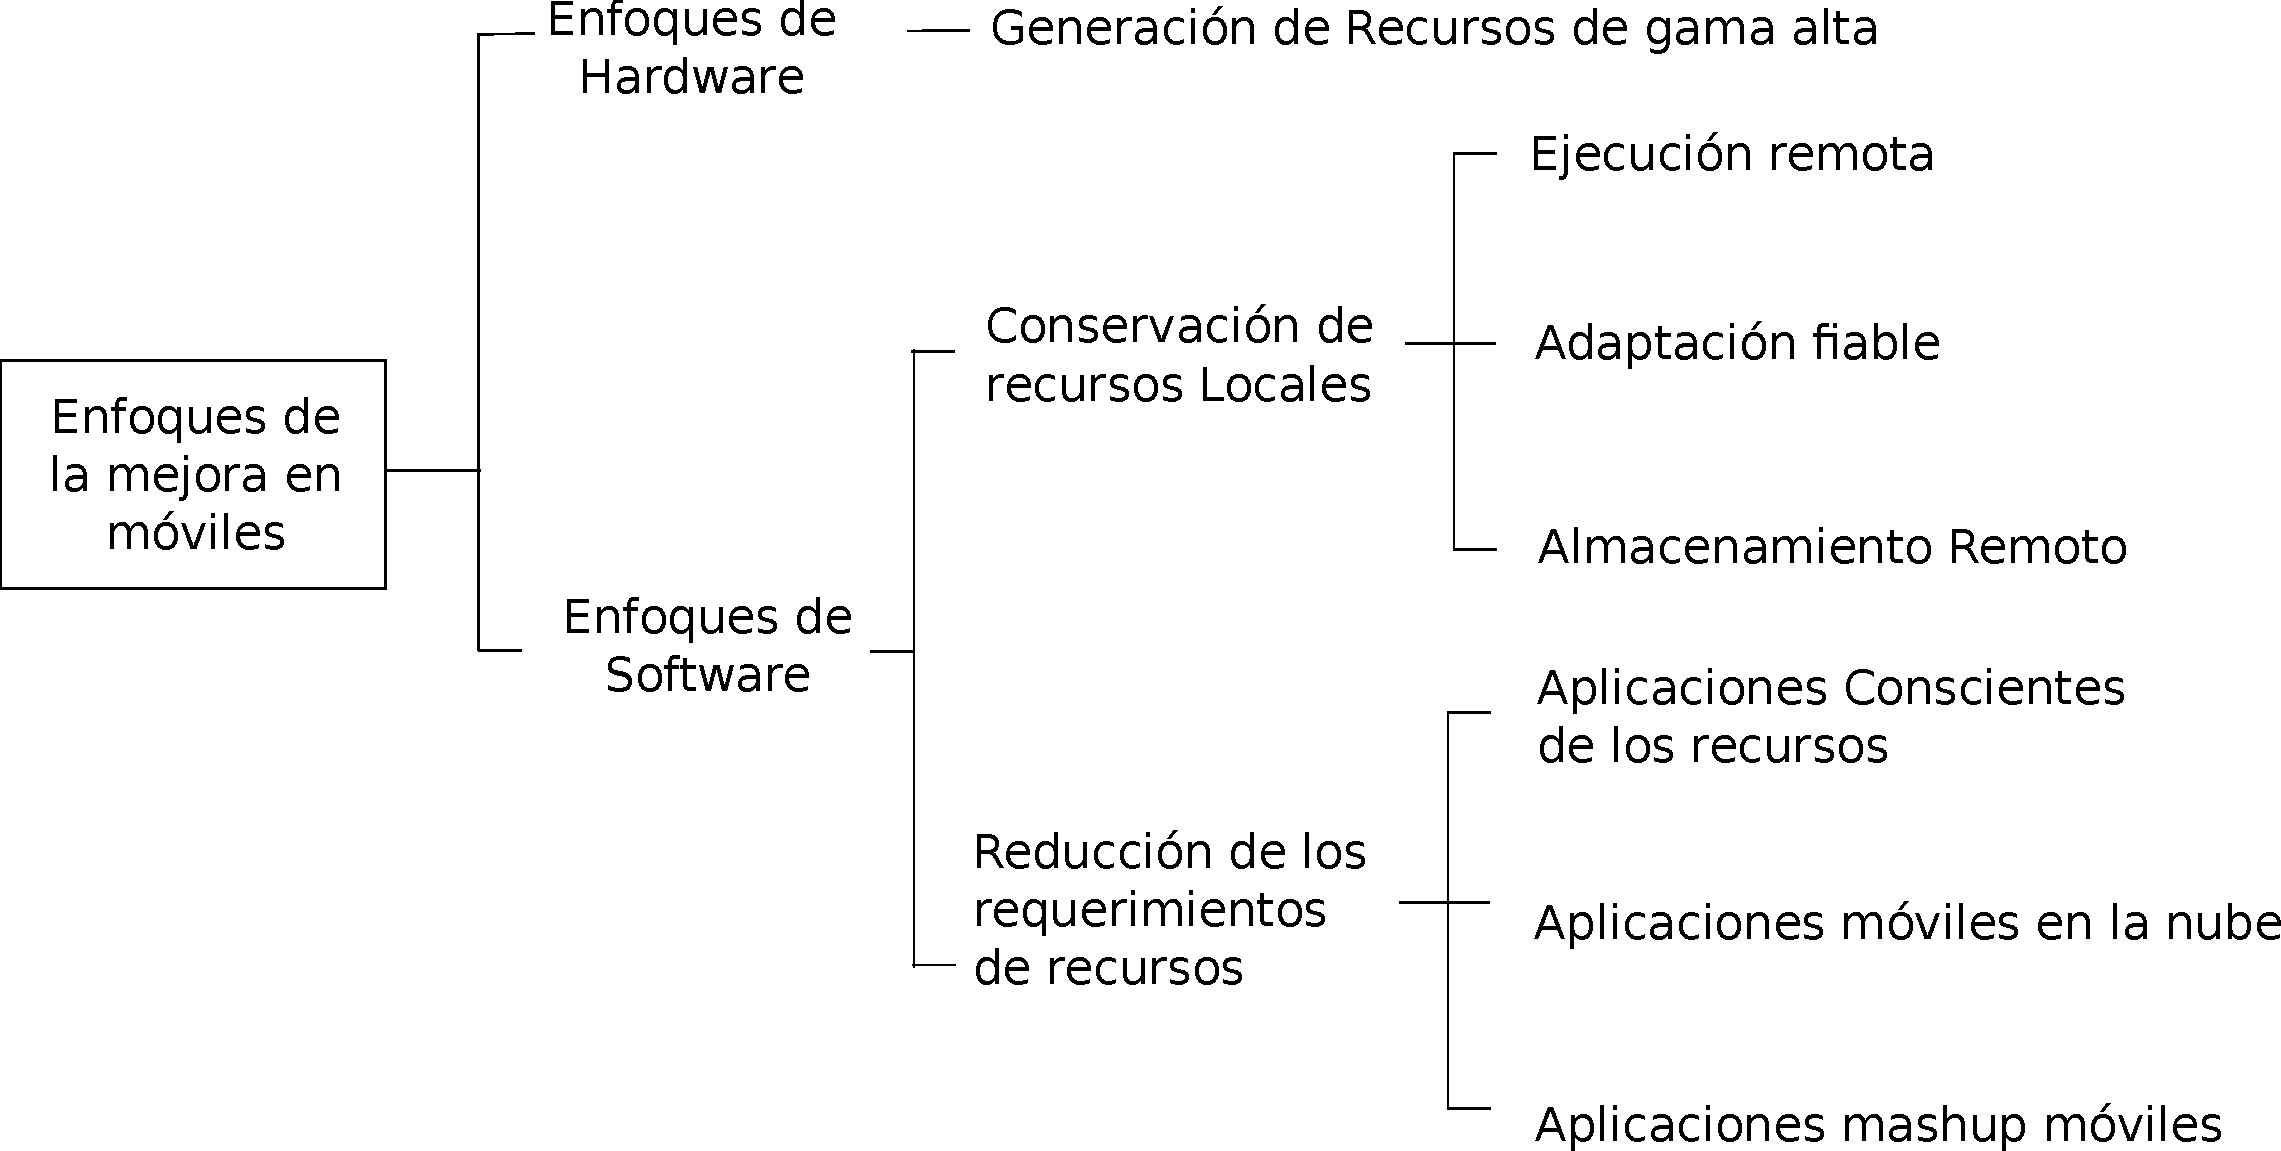
\includegraphics[scale=0.35]{Figures/taxonomySmartphone.pdf}
 \caption{Taxonomía de los enfoques de mejora de en móviles. Figura adaptada de \cite{abolfazli2012mobile}}
 \label{fig:approachesmobileaugmentation}
\end{figure}

\subsection{Heterogeneidad}

La innegable popularidad que han tomado los dispositivos móviles como los smartphones, wereables y objetos de IoT crea un mercado dinámico
y exigente, que ha diversificado a los componentes de MCC en diferentes dimensiones de una manera no estándar. Esta variedad de hardware, arquitecturas,
infraestructura y tecnologías de dispositivos móviles, nubes, y redes inalámbricas genera un entorno Heterogéneo. En esta sección
describimos como la heterogeneidad abarca a todos los componentes de MCC: computación móvil, computación en nube y redes inalámbricas
\cite{sanaei2014heterogeneity}. Este
escenario es representado en la Figura \ref{fig:mccheterogeinity}. Aunque la heterogeneidad en la MCC ha sido inherente desde los orígenes
de la computación en nube y móvil, su complejidad la hace desafiante y única, por lo que necesita un estudio exhaustivo.


\begin{figure}[h]
 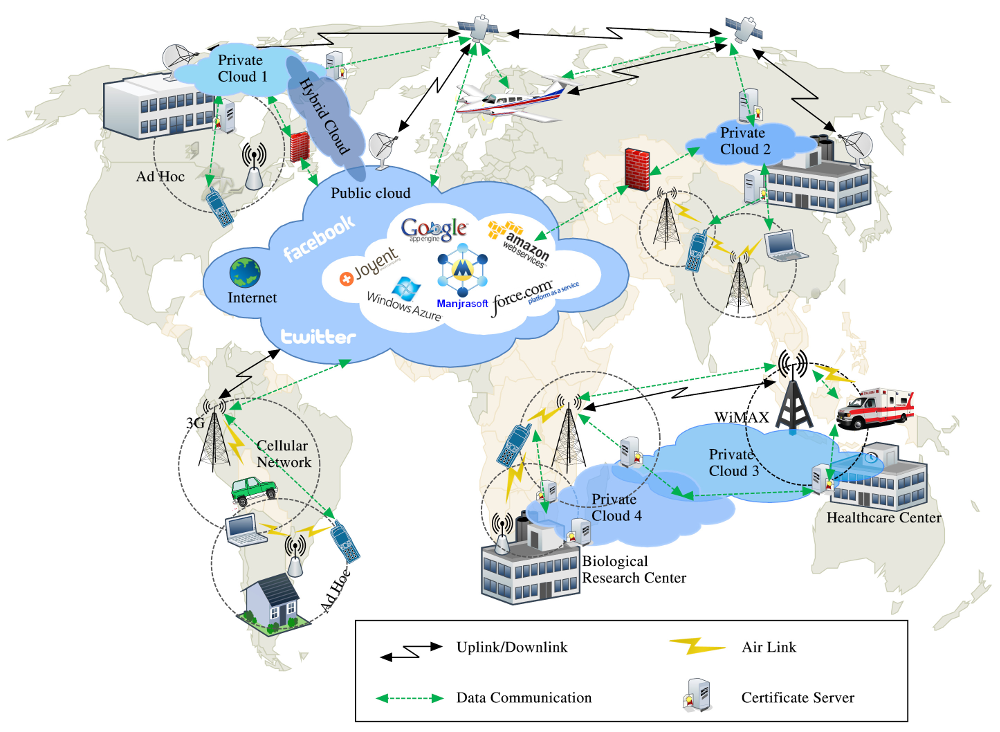
\includegraphics[scale=0.45]{Figures/mccheterogeinity}
 \caption{Una vista general a MCC \cite{sanaei2014heterogeneity}}
 \label{fig:mccheterogeinity}
\end{figure}

\subsubsection{Taxonomía de la heterogeneidad en MCC}

Para entender claramente la heterogeneidad que no es una característica específica de un dominio, podemos percibir casos en la vida real:
los automóviles que están compuestos de partes totalmente diferentes que logran interactuar entre ellos con un solo fin; el caso de las
partes del cuerpo que
son intrínsecamente heterogéneas logran cooperan para mantener la funcionalidad como un todo. Análogamente, los tres componentes principales 
de la MCC (computación en la nube, computación móvil y redes inalámbricas) deben interactuar sin problemas y consistentemente. Esta división 
de los orígenes de la taxonomía está representada en la imagen de la Figura \ref{fig:heterogeinityRootsmcc}. 


\begin{figure}[h]
 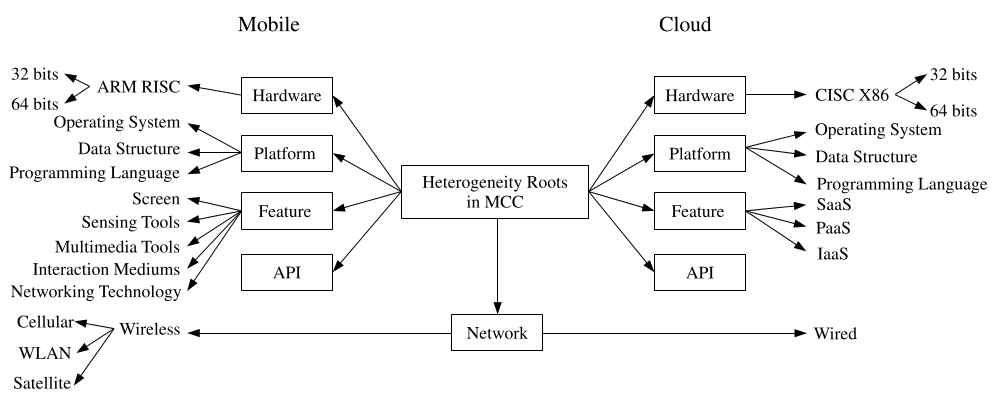
\includegraphics[scale=0.45]{Figures/heterogeinityRootsmcc}
 \caption{Taxonomía de los orígenes de la heterogeneidad en MCC \cite{sanaei2014heterogeneity}}
 \label{fig:heterogeinityRootsmcc}
\end{figure}


\begin{enumerate}
 \item \textbf{Heterogeneidad de hardware:} La fuerte demanda de los usuarios de móviles y la competencia entre las grandes compañías 
 fabricantes de hardware han permitido que diversifiquen sus arquitecturas internas entre dispositivos móviles, servidores en nube, e 
 infraestructuras de redes. 
 
 En el entorno de la computación en nube, la variedad de proveedores de servidores otorgan una variedad en infraestructuras y diseño 
 de arquitecturas de Computadoras con un Conjunto de Instrucciones Complejas (CISC, por sus siglas en inglés) con las variaciones de 32 y
 64 bits. 
 
 Similarmente, la diversidad de arquitecturas en los dispositivos móviles, que generalmente están basadas en Computadoras con Conjunto de Instrucciones
 Reducidas (RISC, por sus siglas en inglés) de 32 bits; sin embargo, existe una considerable variación en términos de velocidad del procesador,
 número de nucleos, cantidad de caché del procesador. Igualmente existe una variedad importante entre los recursos del dispositivo móvil como
 la memoria memoria interna, fiabilidad de la antena inalámbrica y la capacidad de la batería.
 
 La heterogeneidad en hardware entre los dispositivos móviles y las computación en nube, crea los siguientes problemas: 
 
 \begin{itemize}
  \item La variación de hardware de los servidores en nube conlleva a una diferencia de rendimiento y calidad de servicio, además  del casi nulo
  soporte para la portabilidad de aplicaciones entre los diferentes proveedores, entonces fuerza al usuario a tomar una decisión 
  importante entre la vasta cantidad de opciones disponibles. Los desarrolladores pueden usar la herramienta en línea de \textit{Software Insider}
  para optar por la mejor propuesta de servicios en nube \footnote{\url{http://cloud-computing.softwareinsider.com}, último acceso en setiembre 2015}.
  \item El conocido principio usado por desarrolladores ``codifica una vez, ejecútalo donde sea'' se cumple parcialmente en el 
  heterogéneo ambiente móvil, dado que requiere dependencia de herramientas privadas  
  multi-plataforma como Xamarin \footnote{ \url{http://xamarin.com/}, último acceso en setiembre 2015} o Qt para móviles 
  \footnote{ \url{http://www.qt.io/mobile-app-development/}, último acceso en setiembre 2015}
  . Las herramientas en mención son un gran aporte en el entorno de los \textit{smartphones} pero tienen
  una limitante en entornos de dispositivos \textit{weareables} y de Internet de las cosas, ya que en su arquitectura se ejecuta sobre diferentes
  distribuciones ligeras de Linux.
  \item Un parámetro fundamental en las técnicas de \textit{offloading} es la estimación precisa de la energía \cite{sanaei2014heterogeneity},
  para
  que se decida si el enviar partes de la aplicación conservará energía o no \cite{5445167}. Es por tal motivo que se necesita estimar de manera precisa
  este valor 
  
 \end{itemize}

 \item \textbf{Heterogeneidad de Plataforma:} De modo equivalente a la heterogeneidad de hardware, existe una amplia disponibilidad de sistemas
 operativos, lenguajes de programación y estructuras de datos en MCC que transforman a las plataformas en entornos heterogéneos. En el contexto
 de los sistemas operativos móviles encontramos algunos como Android \footnote{\url{http://developer.android.com/index.html}, último acceso en setiembre 2015} y iOS 
 \footnote{\url{https://developer.apple.com/devcenter/ios/index.action}, último acceso en setiembre 2015}, de Google y Apple respectivamente,
 cada uno con múltiples versiones
 y  arquitecturas que soportan diferentes lenguajes de programación y estructuras de datos. Android ofrece el desarrollo sobre la máquina virtual 
 de java basado en bytecodes; mientras que iOS soporta Objective-C, un lenguaje compilado a nivel de código máquina.
 
 En en ámbito de la computación en nube los proveedores más populares tales como App Engine
 \footnote{\url{https://cloud.google.com/appengine/docs}, último acceso en setiembre 2015}, Microsoft Azure
 \footnote{\url{https://azure.microsoft.com/en-us/}, último acceso en setiembre 2015} y 
 Amazon Web Services \footnote{\url{http://aws.amazon.com/}, último acceso en setiembre 2015} soportan una diversa cantidad de lenguajes de programación, sistemas operativos
 y arquitecturas de almacenamiento, p. ej. Azure Soporta .Net, PHP, Ruby, Python y Java para desarrollar aplicaciones, Google 
 igualmente ofrece Java además de Python, PHP y Go; sin embargo, estas plataformas poseen almacenes de datos no relacionales con diseños 
 estructurales y esquemas de particionado diferentes (Big table de Google \cite{Chang:2006:BDS:1267308.1267323}, Dynamo de Amazon \cite{decandia2007dynamo} y 
 DocumentDB de Azure 
 \footnote{\url{http://azure.microsoft.com/en-us/services/documentdb/}, último acceso en setiembre 2015}), y por lo tanto estos proveedores hacen cumplir  sus restricciones
 de uso  para proveer mayor flexibilidad de su servicio.
 
 Tal heterogeneidad convierte la portabilidad en un proceso tedioso, costoso y de alto riesgo. Transferir aplicaciones entre diferentes
 nubes demanda un costo extra que incluye descargar la aplicación, realizar la conversión y desplegar el nuevo sistema a la nueva nube. Es
 peligroso, dado que la transferencia entre bases de datos de entre nubes compromete la privacidad e integridad de los datos cuando existe una
 diferencia entre sistemas de archivos y técnicas de encriptación \cite{5708456}. Por lo tanto, para el desarrollador escoger la plataforma 
 correcta no es tarea fácil. La variedad de plataformas se representa en la Figura \ref{fig:difficultDecisiton}.
 
 \begin{figure}[h]
 \centering 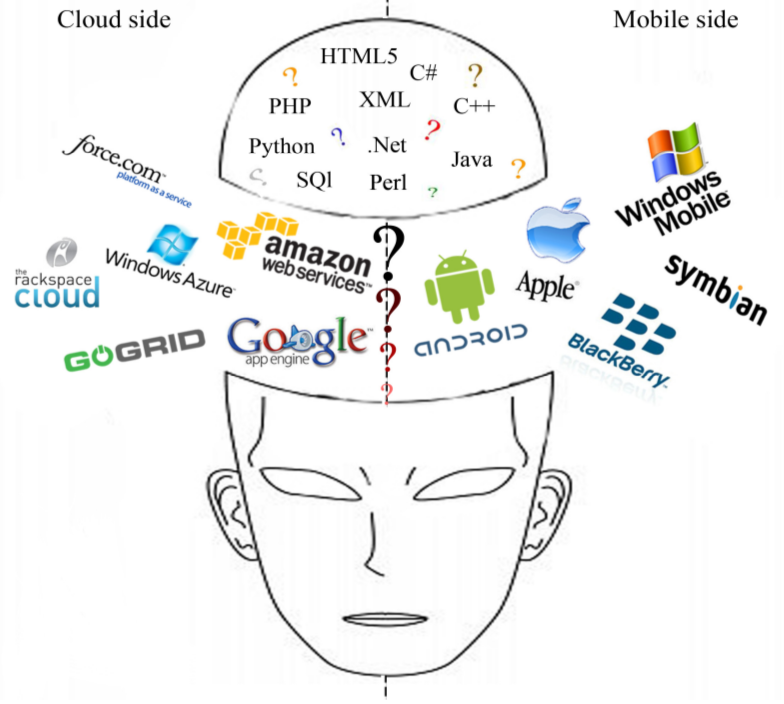
\includegraphics[scale=0.3]{Figures/difficultDecisiton}
 \caption{Heterogeneidad de plataformas en MCC y la difícil tarea para el desarrollador elegir la correcta \cite{sanaei2014heterogeneity}}
 \label{fig:difficultDecisiton}
\end{figure}
 
 %falta un poco hablar de las soluciones como phonegap o marmalade
 
 % La portabilidad como la define el Comité Internacional para los Estándares de Tecnologías de la Información (INCITS, por sus siglas en inglés) 

 
 \item \textbf{Heterogeneidad de Características: } Es la variación de características en los \textit{smartphones} tales como los sensores,
 el área de visualización,  multimedia, y tecnologías de red. Una de las características que más varía entre fabricantes es la cámara. P. ej.
 El celular motorola X, un celular de gama media, posee una cámara de 10PM \footnote{\url{https://www.motorola.com/us/Moto-X/FLEXR1.html}, 
 último acceso en setiembre 2015}, entretanto 
 el celular Samsung Galaxy Edge 6, un celular de gama alta, dispone de una cámara de 16 MP \footnote{\url{http://www.samsung.com/uk/galaxys6/}, 
 último acceso en setiembre 2015}. Esta
 desigualdad puede significar una variación en las técnicas de offloading ( las cuales detallaremos en el Capítulo \ref{ch:Chapter4}) 
 si es que consideramos algún tipo de procesamiento de imagen en la nube,  debido a que el envío de datos a la nube sería más lento.
 
 Las variaciones en el área de visualización entre los celulares impiden que los desarrolladores diseñar una interfaz de usuario que se adapte a 
 todos los tamaños de pantalla, disminuyendo la experiencia de usuario.	En el entorno Android existe el soporte para la construcción de 
 aplicaciones que se adecúan al contenido de la pantalla en su versión 3.2 en adelante \footnote{
 \url{http://developer.android.com/about/versions/android-3.2.html}, último acceso en setiembre 2015}.
 
 La heterogeneidad en nube está dada por los servicios que cada proveedor ofrece en particular. P. ej. \textit{Google App Engine} ofrece el servicio 
 de Big Query \footnote{\url{https://cloud.google.com/bigquery/}, último acceso en setiembre 2015} que permite a los administradores
 realizar consultas sobre \textit{Big Data} 
 en tiempo real. Microsoft Azure a su vez, es el único que ofrece un servicio de almacenamiento de backups encriptado 
 \footnote{\url{http://azure.microsoft.com/en-us/services/backup/}, último acceso en setiembre 2015} 
  
  \item \textbf{Heterogeneidad de APIs:} Las Interfaces de Programación de Aplicaciones (API, por sus siglas en inglés) son bibliotecas de código
  que permiten un acceso rápido a datos específicos o funciones de un proveedor en particular. Los usuarios de \textit{smartphones} tienen una 
  alta expectativa respecto a la experiencia de usuario, es por tal motivo que las mas grandes compañías de sistemas operativos móviles (Android, iOS, 
  Blackberry \footnote{\url{http://us.blackberry.com/}, último acceso en setiembre 2015} y Firefox OS 
  \footnote{\url{https://www.mozilla.org/en-US/firefox/os/2.0/}, último acceso en setiembre 2015}) otorgan una amplia
  gama de APIs a los desarrolladores. Esta es una ventaja para desarrollar aplicaciones enriquecedoras en experiencia de usuario, de una forma 
  ágil y fácil sin necesidad de acceder al kernel. Sin embargo, las APIs son dependientes de los proveedores y la portabilidad nuevamente se
  convierte en una tarea complicada, dadas las diferencias de las APIs.
  
  De manera similar, en la computación en nube, la casi totalidad de proveedores diseñan APIs que son usados exclusivamente por sus clientes
  p. ej. Google App engine ofrece la API de documentos e Indices \footnote{\url{https://cloud.google.com/appengine/docs/java/search/}, último acceso en setiembre 2015} 
  para realizar búsquedas de manera rápida y eficiente sobre espacios geográficos y texto principalmente. Otro ejemplo que resaltamos es 
  en el envío de notificaciones push, Google, Azure y Parse \footnote{\url{https://www.parse.com/}, último acceso en setiembre 2015}
  ofrecen sus APIs basadas en 
  \textit{Google Cloud Messaging} \footnote{\url{https://developer.android.com/google/gcm/index.html}, último acceso en setiembre 2015}
  , \textit{Notification Hubs} 
  \footnote{\url{http://azure.microsoft.com/en-us/documentation/services/notification-hubs/}, último acceso en agosto 2015} y \textit{Parse Push Notifications} 
  \footnote{\url{https://parse.com/docs/push_guide}, último acceso en julio 2015} respectivamente. Esta heterogeneidad además que impide la portabilidad, 
  demanda un tiempo considerable al desarrollador poder aprender cada una de las APIs en nube.
  
  \item \textbf{Heterogeneidad de Redes:} A diferencia de las computadoras de escritorio, la mayoría de dispositivos móviles solamente usan redes
  inalámbricas para conectarse a Internet, las cuales son comparativamente más intermitentes y menos fiables. La variedad infraestructuras
  de redes inalámbricas disponibles como Wi-fi, 3G y 4G dificultan el proceso de selección de la red más adecuada en el momento que el cliente
  móvil está en movimiento.
  
 
\end{enumerate}






 
%% Chapter 2

\chapter{Computación en Nube para Móviles} % Main chapter title

\label{Chapter3} % For referencing the chapter elsewhere, use \ref{Chapter1} 

\lhead{Capítulo 3. \emph{Computación en nube para móviles}} % This is for the header on each page - perhaps a shortened title

%----------------------------------------------------------------------------------------

El área de la computación en nube para móviles al ser un campo de investigación relativamente nuevo, no existe una definición
ampliamente aceptada y puede ser vista desde muchos ángulos como lo realizó el trabajo de  Fernando, Loke y Rahayu 
\cite{fernando2013mobile}, tomando hasta 3 definiciones distintas. En este trabajo nos referimos a MCC como un conjunto de técnicas que 
aprovechan los potentes recursos computacionales en nube para potenciar aplicaciones móviles con el principal objetivo de mejorar la calidad de 
servicio hacia los usuarios que tienen dispositivos limitados en términos de energía, procesamiento y almacenamiento. En este capítulo
detallaremos la visión actual de MCC, del mismo modo explicaremos la heterogeneidad que la envuelve,
y los desafíos por solucionar en las técnicas de \textit{offloading}.

\section{Visión}

MCC permite a los usuarios móviles acceder a sus aplicaciones, datos, y servicios en nube a través de internet aprovechando 
la web móvil \cite{dinh2013survey}, consiguiendo no depender totalmente de los recursos locales de los móviles,
, por tanto esta nueva ola tecnológica puede ser aplicada en varias áreas como la salud, negocios de TI, educación,
entretenimiento y redes sociales. 

En el trabajo de Abolfazli, Sanaei y Gani \cite{abolfazli2012mobile} se clasifica los enfoques
que puede tomar la mejora en los dispositivos móviles entre hardware y software los cuales se muestran en la gráfica de la Figura
\ref{fig:approachesmobileaugmentation}.  Si bien los avances de hardware son virtuosos, son aún lentos en comparación a la creciente 
expectativa de los usuarios y desarrolladores de aplicaciones. Otro enfoque alternativo para la mejora de las capacidades computacionales 
de los dispositivos es usar técnicas de software 
para la conservación de recursos
locales y la reducción de requerimientos de recursos al instalar aplicaciones. En consecuencia, sostenemos que la computación en nube 
tendrá una participación
destacada aventajándose de valiosos recursos remotos con el fin de mejorar la experiencia del usuario.

\begin{figure}[h]
 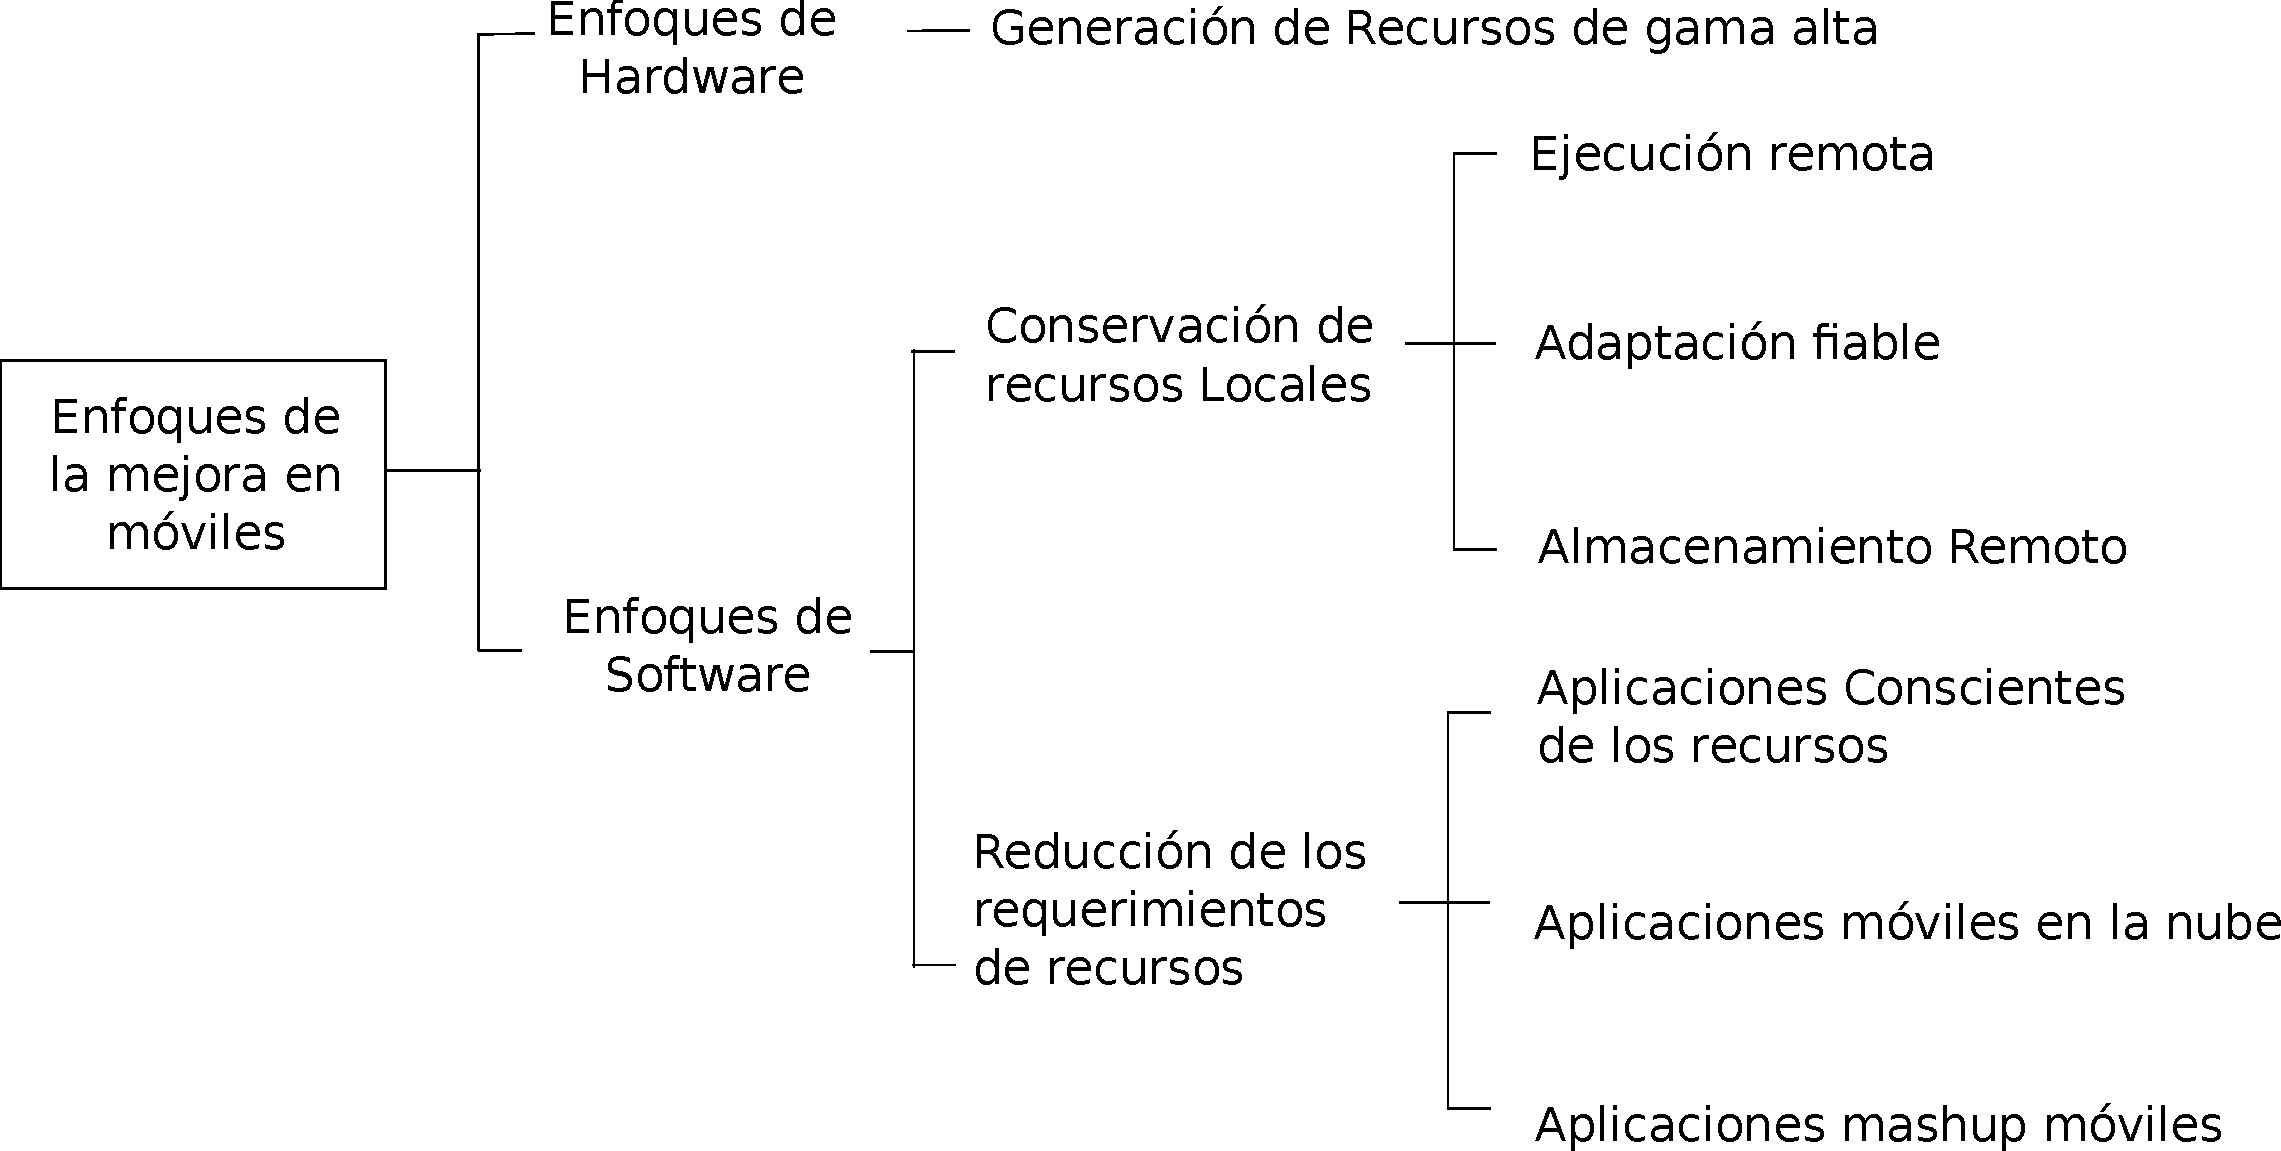
\includegraphics[scale=0.35]{Figures/taxonomySmartphone.pdf}
 \caption{Taxonomía de los enfoques de mejora de en móviles. Figura adaptada de \cite{abolfazli2012mobile}}
 \label{fig:approachesmobileaugmentation}
\end{figure}

\section{Heterogeneidad}

La innegable popularidad que han tomado los dispositivos móviles como los smartphones, wereables y objetos de IoT crea un mercado dinámico
y exigente, que ha diversificado a los componentes de MCC en diferentes dimensiones de una manera no estándar. Esta variedad de hardware, arquitecturas,
infraestructura y tecnologías de dispositivos móviles, nubes, y redes inalámbricas genera un entorno Heterogéneo. En esta sección
describimos como la heterogeneidad abarca a todos los componentes de MCC: computación móvil, computación en nube y redes inalámbricas
\cite{sanaei2014heterogeneity}. Este
escenario es representado en la Figura \ref{fig:mccheterogeinity}. Aunque la heterogeneidad en la MCC ha sido inherente desde los orígenes
de la computación en nube y móvil, su complejidad la hace desafiante y única, por lo que necesita un estudio exhaustivo.


\subsection{Taxonomía en la MCC}

En este apartado estudiaremos detalladamente la heterogeneidad en MCC por medio del análisis de sus orígenes y dimensiones. 
Según \cite{sanaei2014heterogeneity}, 
los orígenes de la heterogeneidad se dan por el hardware, plataforma, característica, API, red y dispositivos. 


\begin{figure}[h]
 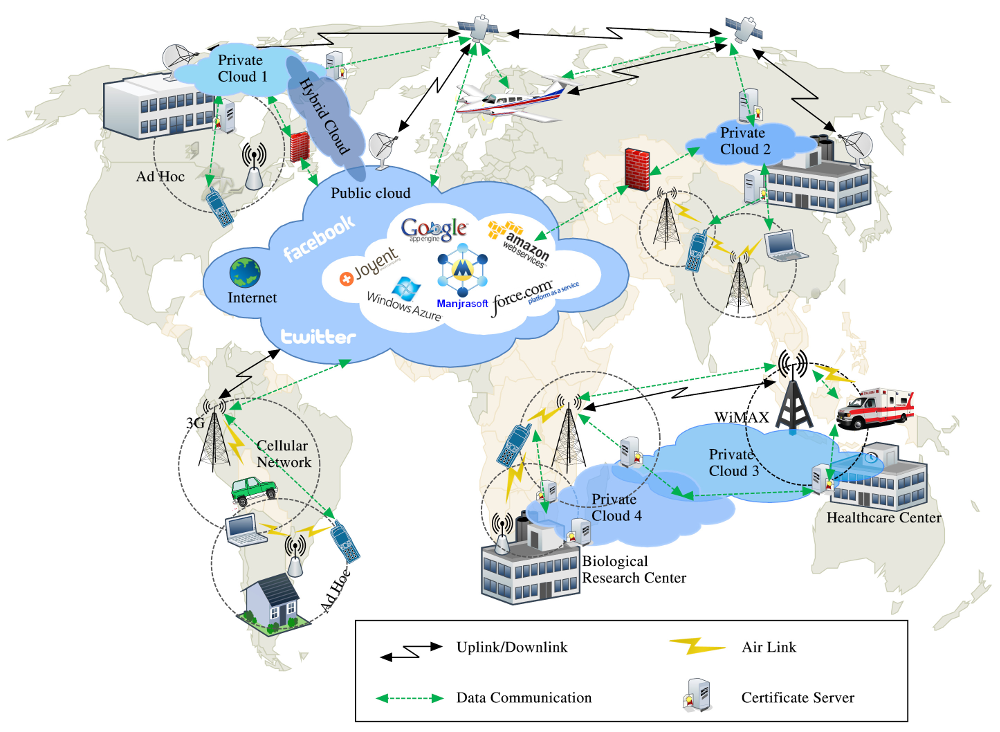
\includegraphics[scale=0.45]{Figures/mccheterogeinity}
 \caption{Una vista general a MCC \cite{sanaei2014heterogeneity}}
 \label{fig:mccheterogeinity}
\end{figure}

\subsubsection{Orígenes de la heterogeneidad en MCC}

Para entender claramente la heterogeneidad que no es una característica específica de un dominio, podemos percibir casos en la vida real:
los automóviles que están compuestos de partes totalmente diferentes que logran interactuar entre ellos con un solo fin; el caso de las
partes del cuerpo que
son intrínsecamente heterogéneas logran cooperan para mantener la funcionalidad como un todo. Análogamente, los tres componentes principales 
de la MCC (computación en la nube, computación móvil y redes inalámbricas) deben interactuar sin problemas y consistentemente. Esta división 
de los orígenes de la taxonomía está representada en la imagen de la Figura \ref{fig:heterogeinityRootsmcc}. 


\begin{figure}[h]
 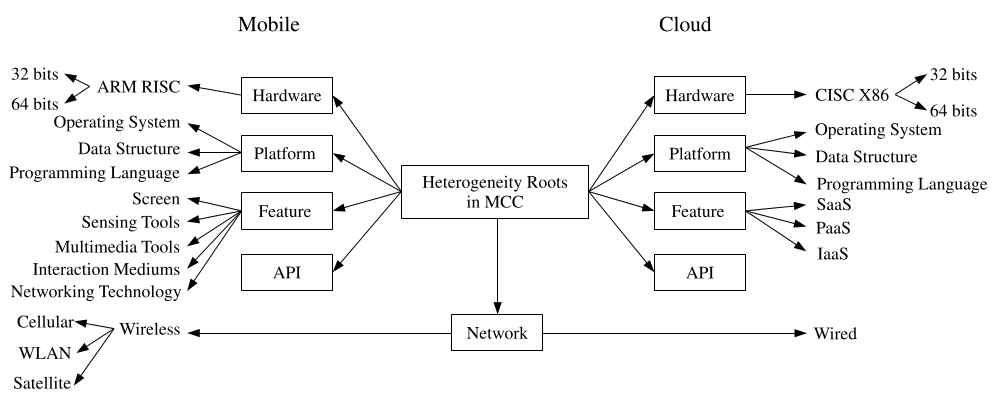
\includegraphics[scale=0.45]{Figures/heterogeinityRootsmcc}
 \caption{Taxonomía de los orígenes de la heterogeneidad en MCC \cite{sanaei2014heterogeneity}}
 \label{fig:heterogeinityRootsmcc}
\end{figure}


\begin{enumerate}
 \item \textbf{Heterogeneidad de hardware:} La fuerte demanda de los usuarios de móviles y la competencia entre las grandes compañías 
 fabricantes de hardware han permitido que diversifiquen sus arquitecturas internas entre dispositivos móviles, servidores en nube, e 
 infraestructuras de redes. 
 
 En el entorno de la computación en nube, la variedad de proveedores de servidores otorgan una variedad en infraestructuras y diseño 
 de arquitecturas de Computadoras con un Conjunto de Instrucciones Complejas (CISC, por sus siglas en inglés) con las variaciones de 32 y
 64 bits. 
 
 Similarmente, la diversidad de arquitecturas en los dispositivos móviles, que generalmente están basadas en Computadoras con Conjunto de Instrucciones
 Reducidas (RISC, por sus siglas en inglés) de 32 bits; sin embargo, existe una considerable variación en términos de velocidad del procesador,
 número de nucleos, cantidad de caché del procesador. Igualmente existe una variedad importante entre los recursos del dispositivo móvil como
 la memoria memoria interna, fiabilidad de la antena inalámbrica y la capacidad de la batería.
 
 La heterogeneidad en hardware entre los dispositivos móviles y las computación en nube, crea los siguientes problemas: 
 
 \begin{itemize}
  \item La variación de hardware de los servidores en nube conlleva a una diferencia de rendimiento y calidad de servicio, además  del casi nulo
  soporte para la portabilidad de aplicaciones entre los diferentes proveedores, entonces fuerza al usuario a tomar una decisión 
  importante entre la vasta cantidad de opciones disponibles. Los desarrolladores pueden usar la herramienta en línea de \textit{Software Insider}
  para optar por la mejor propuesta de servicios en nube \footnote{\url{http://cloud-computing.softwareinsider.com}, último acceso en setiembre 2015}.
  \item El conocido principio usado por desarrolladores ``codifica una vez, ejecútalo donde sea'' se cumple parcialmente en el 
  heterogéneo ambiente móvil, dado que requiere dependencia de herramientas privadas  
  multi-plataforma como Xamarin \footnote{ \url{http://xamarin.com/}, último acceso en setiembre 2015} o Qt para móviles 
  \footnote{ \url{http://www.qt.io/mobile-app-development/}, último acceso en setiembre 2015}
  . Las herramientas en mención son un gran aporte en el entorno de los \textit{smartphones} pero tienen
  una limitante en entornos de dispositivos \textit{weareables} y de Internet de las cosas, ya que en su arquitectura se ejecuta sobre diferentes
  distribuciones ligeras de Linux.
  \item Un parámetro fundamental en las técnicas de \textit{offloading} es la estimación precisa de la energía \cite{sanaei2014heterogeneity},
  para
  que se decida si el enviar partes de la aplicación conservará energía o no \cite{5445167}. Es por tal motivo que se necesita estimar de manera precisa
  este valor 
  
 \end{itemize}

 \item \textbf{Heterogeneidad de Plataforma:} De modo equivalente a la heterogeneidad de hardware, existe una amplia disponibilidad de sistemas
 operativos, lenguajes de programación y estructuras de datos en MCC que transforman a las plataformas en entornos heterogéneos. En el contexto
 de los sistemas operativos móviles encontramos algunos como Android \footnote{\url{http://developer.android.com/index.html}, último acceso en setiembre 2015} y iOS 
 \footnote{\url{https://developer.apple.com/devcenter/ios/index.action}, último acceso en setiembre 2015}, de Google y Apple respectivamente,
 cada uno con múltiples versiones
 y  arquitecturas que soportan diferentes lenguajes de programación y estructuras de datos. Android ofrece el desarrollo sobre la máquina virtual 
 de java basado en bytecodes; mientras que iOS soporta Objective-C, un lenguaje compilado a nivel de código máquina.
 
 En en ámbito de la computación en nube los proveedores más populares tales como App Engine
 \footnote{\url{https://cloud.google.com/appengine/docs}, último acceso en setiembre 2015}, Microsoft Azure
 \footnote{\url{https://azure.microsoft.com/en-us/}, último acceso en setiembre 2015} y 
 Amazon Web Services \footnote{\url{http://aws.amazon.com/}, último acceso en setiembre 2015} soportan una diversa cantidad de lenguajes de programación, sistemas operativos
 y arquitecturas de almacenamiento, p. ej. Azure Soporta .Net, PHP, Ruby, Python y Java para desarrollar aplicaciones, Google 
 igualmente ofrece Java además de Python, PHP y Go; sin embargo, estas plataformas poseen almacenes de datos no relacionales con diseños 
 estructurales y esquemas de particionado diferentes (Big table de Google \cite{Chang:2006:BDS:1267308.1267323}, Dynamo de Amazon \cite{decandia2007dynamo} y 
 DocumentDB de Azure 
 \footnote{\url{http://azure.microsoft.com/en-us/services/documentdb/}, último acceso en setiembre 2015}), y por lo tanto estos proveedores hacen cumplir  sus restricciones
 de uso  para proveer mayor flexibilidad de su servicio.
 
 Tal heterogeneidad convierte la portabilidad en un proceso tedioso, costoso y de alto riesgo. Transferir aplicaciones entre diferentes
 nubes demanda un costo extra que incluye descargar la aplicación, realizar la conversión y desplegar el nuevo sistema a la nueva nube. Es
 peligroso, dado que la transferencia entre bases de datos de entre nubes compromete la privacidad e integridad de los datos cuando existe una
 diferencia entre sistemas de archivos y técnicas de encriptación \cite{5708456}. Por lo tanto, para el desarrollador escoger la plataforma 
 correcta no es tarea fácil. La variedad de plataformas se representa en la Figura \ref{fig:difficultDecisiton}.
 
 \begin{figure}[h]
 \centering 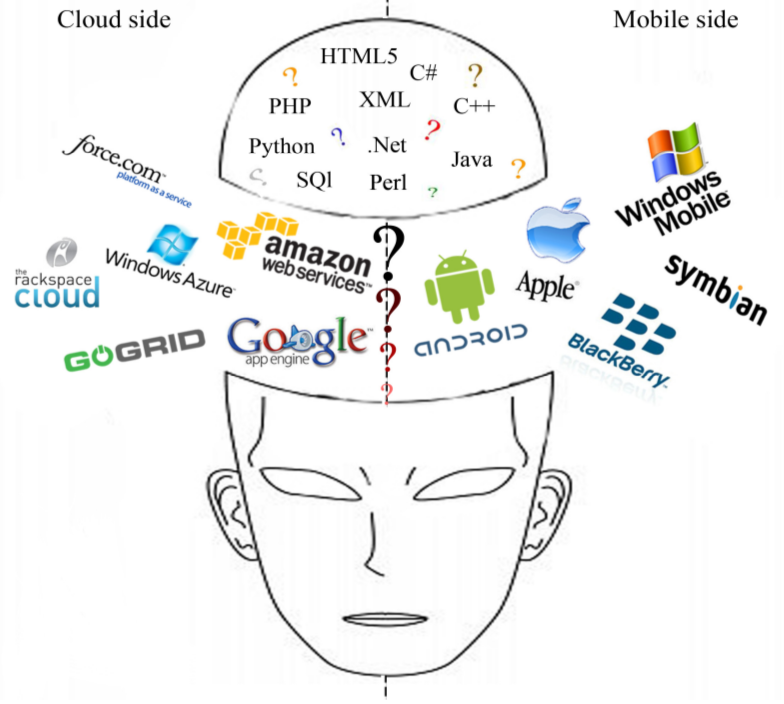
\includegraphics[scale=0.3]{Figures/difficultDecisiton}
 \caption{Heterogeneidad de plataformas en MCC y la difícil tarea para el desarrollador elegir la correcta \cite{sanaei2014heterogeneity}}
 \label{fig:difficultDecisiton}
\end{figure}
 
 %falta un poco hablar de las soluciones como phonegap o marmalade
 
 % La portabilidad como la define el Comité Internacional para los Estándares de Tecnologías de la Información (INCITS, por sus siglas en inglés) 

 
 \item \textbf{Heterogeneidad de Características: } Es la variación de características en los \textit{smartphones} tales como los sensores,
 el área de visualización,  multimedia, y tecnologías de red. Una de las características que más varía entre fabricantes es la cámara. P. ej.
 El celular motorola X, un celular de gama media, posee una cámara de 10PM \footnote{\url{https://www.motorola.com/us/Moto-X/FLEXR1.html}, 
 último acceso en setiembre 2015}, entretanto 
 el celular Samsung Galaxy Edge 6, un celular de gama alta, dispone de una cámara de 16 MP \footnote{\url{http://www.samsung.com/uk/galaxys6/}, 
 último acceso en setiembre 2015}. Esta
 desigualdad puede significar una variación en las técnicas de offloading ( las cuales detallaremos en el Capítulo \ref{ch:Chapter4}) 
 si es que consideramos algún tipo de procesamiento de imagen en la nube,  debido a que el envío de datos a la nube sería más lento.
 
 Las variaciones en el área de visualización entre los celulares impiden que los desarrolladores diseñar una interfaz de usuario que se adapte a 
 todos los tamaños de pantalla, disminuyendo la experiencia de usuario.	En el entorno Android existe el soporte para la construcción de 
 aplicaciones que se adecúan al contenido de la pantalla en su versión 3.2 en adelante \footnote{
 \url{http://developer.android.com/about/versions/android-3.2.html}, último acceso en setiembre 2015}.
 
 La heterogeneidad en nube está dada por los servicios que cada proveedor ofrece en particular. P. ej. \textit{Google App Engine} ofrece el servicio 
 de Big Query \footnote{\url{https://cloud.google.com/bigquery/}, último acceso en setiembre 2015} que permite a los administradores
 realizar consultas sobre \textit{Big Data} 
 en tiempo real. Microsoft Azure a su vez, es el único que ofrece un servicio de almacenamiento de backups encriptado 
 \footnote{\url{http://azure.microsoft.com/en-us/services/backup/}, último acceso en setiembre 2015} 
  
  \item \textbf{Heterogeneidad de APIs:} Las Interfaces de Programación de Aplicaciones (API, por sus siglas en inglés) son bibliotecas de código
  que permiten un acceso rápido a datos específicos o funciones de un proveedor en particular. Los usuarios de \textit{smartphones} tienen una 
  alta expectativa respecto a la experiencia de usuario, es por tal motivo que las mas grandes compañías de sistemas operativos móviles (Android, iOS, 
  Blackberry \footnote{\url{http://us.blackberry.com/}, último acceso en setiembre 2015} y Firefox OS 
  \footnote{\url{https://www.mozilla.org/en-US/firefox/os/2.0/}, último acceso en setiembre 2015}) otorgan una amplia
  gama de APIs a los desarrolladores. Esta es una ventaja para desarrollar aplicaciones enriquecedoras en experiencia de usuario, de una forma 
  ágil y fácil sin necesidad de acceder al kernel. Sin embargo, las APIs son dependientes de los proveedores y la portabilidad nuevamente se
  convierte en una tarea complicada, dadas las diferencias de las APIs.
  
  De manera similar, en la computación en nube, la casi totalidad de proveedores diseñan APIs que son usados exclusivamente por sus clientes
  p. ej. Google App engine ofrece la API de documentos e Indices \footnote{\url{https://cloud.google.com/appengine/docs/java/search/}, último acceso en setiembre 2015} 
  para realizar búsquedas de manera rápida y eficiente sobre espacios geográficos y texto principalmente. Otro ejemplo que resaltamos es 
  en el envío de notificaciones push, Google, Azure y Parse \footnote{\url{https://www.parse.com/}, último acceso en setiembre 2015}
  ofrecen sus APIs basadas en 
  \textit{Google Cloud Messaging} \footnote{\url{https://developer.android.com/google/gcm/index.html}, último acceso en setiembre 2015}
  , \textit{Notification Hubs} 
  \footnote{\url{http://azure.microsoft.com/en-us/documentation/services/notification-hubs/}, último acceso en agosto 2015} y \textit{Parse Push Notifications} 
  \footnote{\url{https://parse.com/docs/push_guide}, último acceso en julio 2015} respectivamente. Esta heterogeneidad además que impide la portabilidad, 
  demanda un tiempo considerable al desarrollador poder aprender cada una de las APIs en nube.
  
  \item \textbf{Heterogeneidad de Redes:} A diferencia de las computadoras de escritorio, la mayoría de dispositivos móviles solamente usan redes
  inalámbricas para conectarse a Internet, las cuales son comparativamente más intermitentes y menos fiables. La variedad infraestructuras
  de redes inalámbricas disponibles como Wi-fi, 3G y 4G dificultan el proceso de selección de la red más adecuada en el momento que el cliente
  móvil está en movimiento.
  
  
  
 
 
\end{enumerate}


% Chapter 4

\chapter{Offloading de Cómputo} % Main chapter title

\label{ch:Chapter3} % For referencing the chapter elsewhere, use \ref{Chapter1} 

\lhead{Capítulo 3. \emph{Offloading de Cómputo}} % This is for the header on each page - perhaps a shortened title

En los últimos años, los usuarios de dispositivos móviles han sido testigos de un crecimiento considerable de aplicaciones
que son útiles en diferentes áreas: salud, entretenimiento, educación, entre otras. Dichas aplicaciones están disponibles 
(en algunos casos de manera gratuita) en distintas tiendas virtuales como (\emph{Google Play Store} \footnote{\url{https://play.google.com/store}
, último acceso en junio 2015}
, \emph{App Store} \footnote{\url{https://itunes.apple.com/us/genre/ios/id36}, último acceso en junio 2015}
y/o \emph{Amazon App Store} \footnote{\url{http://www.amazon.com/mobile-apps/b?node=2350149011}, último acceso en junio 2015}, entre otras. El crecimiento del mercado de programas móviles según
\emph{Transparency Market Research} ~\cite{transparencymarketresearch2014} (empresa que realiza investigación de mercado electrónico) 
pronostica que el mercado móvil crecerá rápidamente en los próximos cinco años, aumentando su valor en aproximadamente US\$ 16.97 billones
en el año 2014 a una valuación total de US\$ 54.89  billones en el año 2020. 

\begin{comment}
Hoy en día los dispositivos móviles ofrecen a los usuarios más aplicaciones, más y mejor ancho de banda para comunicarse y
más poder de procesamiento, 
los cuales colocan una carga pesada sobre el consumo de energía, mientras que los avances en la capacidad de batería crece en menor proporción
que los requerimientos en software de los usuarios modernos.

Se ha redescubierto que el offloading de computación usando  recursos no móviles disponibles a través de los canales de comunicación puede ayudar 
a reducir y conservar el consumo de energía \cite{5445167}, además que el offloading de aplicaciones puede resultar en tiempos de respuesta más 
rápidos, dado que los recursos remotos poseen mejores recursos de cálculo y almacenamiento que los dispositivos móviles. Este modelo es diferente
a las tradicionales arquitecturas cliente-servidor, en donde un cliente siempre migra el cálculo al servidor. El offloading de computo es diferente
del mismo modo a los modelos de migración usados en los sistemas multiprocesador y computación en grilla, donde un proceso puede ser migrado
para balancear la carga \cite{Powell:CSD-83-132}. La diferencia principal es que el \textit{offloading} migra procesos a servidores fuera del
entorno de computación inmediato al usuario, mientras que en computación en grilla ocurre de una computadora a otra con el mismo entorno 
computacional \cite{raey}.
\end{comment}

El uso intensivo y en conjunto de tales aplicaciones demandan una cantidad importante de procesamiento y de energía, los cuales 
no son abastecidos, esto por las limitaciones en los móviles ~\cite{6157576} : (i) baja capacidad de procesamiento, (ii) memoria limitada,
(iii) conexiones de red inestables, y (iv) duración de la batería limitada; debido a su naturaleza portátil. 

A pesar del gran avance tecnológico en hardware resaltado por la ley de Moore, el recurso más crítico en los dispositivos móviles 
es la densidad de la energía de las baterías, el cual ha tenido una tendencia de mejora considerablemente baja respecto a los demás 
componentes en la computación móvil \cite{1401839}. Tales limitaciones reducen la calidad del servicio 
que los usuarios móviles esperan tener.

La Computación en Nube para móviles (\textit{Mobile Cloud Computing}, MCC) tiene entre sus principales objetivos solucionar tales
inconvenientes proponiendo técnicas y \emph{frameworks} de \emph{offloading} al integrar los recursos en nube al entorno móvil de una
forma elástica y bajo demanda, no solamente para los dispositivos de gama baja sino para cualquier móvil que lo requiera \cite{6553297}. 

En ese escenario, a pesar de que es un área emergente de investigación, la industria móvil ya se ha beneficiado, por ejemplo: 
\begin{itemize}
\item El caso de la aplicación \emph{DeepFace}: El algoritmo de reconocimiento de rostros de \emph{Facebook} que alcanza una precisión del 97.35\%~\cite{taigman2014deepface}; 
\item La aplicación \emph{Google Now} \footnote{\url{http://www.google.com/landing/now/},  último acceso 
en febrero 2015} o \emph{Siri} \footnote{\url{http://www.apple.com/ios/siri/?cid=oas-us}, último acceso 
en febrero 2015 }: Son aplicaciones móviles para Android \footnote{\url{http://developer.android.com/index.html}, último acceso 
en febrero 2015} y iOS \footnote{\url{https://www.apple.com/ios/}, último acceso 
en febrero 2015} respectivamente, que utilizan algoritmos de 
reconocimiento de voz bajo una arquitectura basada en servicios (\textit{Service Oriented Arqchitecture}, SOA).
\item \emph{Dropbox} \footnote{\url{https://www.dropbox.com/}, último acceso en enero 2015},
el  cual permite extender la memoria secundaria del dispositivo en la nube otorgando seguridad de la información en caso de pérdida o robo del dispositivo móvil que lo utiliza, así como también sincronización con los dispositivos enlazados, entre otros beneficios. 
\end{itemize}

La técnica de \emph{Offloading} en el campo de MCC es utilizada para para aumentar virtualmente las capacidades del sistema móvil migrando 
partes de la aplicación a servidores en nube más potentes, de tal forma,  que mejore el tiempo de respuesta, el ahorro de energía y en muchos casos la precisión de los algoritmos. Dicha técnica se encuentra implementada en diferentes {\em frameworks}: MAUI~\cite{Cuervo:2010:MMS:1814433.1814441}, CloneCloud~\cite{chun2011clonecloud}, Cuckoo~\cite{kemp2012cuckoo}, 
COMET~\cite{gordon2012comet}, COFA~\cite{shivarudrappa2011cofa}.

La principal diferencia de estos {\em frameworks} con la arquitectura cliente-servidor es que el cálculo computacional puede o no ser enviado a ejecución remota. Esta decisión es provista por un algoritmo que considera parámetros variables: velocidad de ancho de banda, consumo de energía 
de la interfaz de red, tamaño de datos a enviar, entre otros. También existe una diferencia clave con el modelo \emph{grid computing} ya que las técnicas de \emph{offloading} migran los procesos
a un entorno de computación diferente al del usuario, en tanto que el modelo de \emph{grid} lo hace migrando a otro dentro del mismo entorno computacional. 

Se debe también tener en cuenta la naturaleza heterogénea, la cual es inherente a MCC presentando nuevos retos y desafíos en este nuevo campo de estudio. Debido al crecimiento competitivo de los compañías proveedoras, se generó heterogeneidad entre dispositivos móviles, plataformas de computación en nube y redes inalámbricas, dificultando principalmente la interoperabilidad y portabilidad~\cite{sanaei2014heterogeneity}.

%%%%%%%%%%%%%%%%%%%%%%%%%%%% OFFLOADING %%%%%%%%%%%%%%%%%%%%%%%%%%%%%%
\section{Offloading}
\label{offloading}
El término \emph{offloading} o \emph{cyber-foraging} fue introducido por Satyanarayanan \cite{943998} \emph {``Cyber-foraging es una forma efectiva de lidiar 
con este problema. La idea es aumentar dinámicamente los recursos computacionales de una computadora con conexión inalámbrica aprovechando 
la infraestructura de hardware cableada. A medida que el cálculo es más barato y más abundante, es sensato ``gastar'' estos recursos 
para mejorar la experiencia de usuario ''}.Inicialmente, \emph{Cyber-foraging} propone el aprovechamiento de computadoras estáticas 
en estado inactivo de una red local para aumentar las capacidades de los móviles inalámbricos. Hoy en día, la mayor estabilidad de las redes 
inalámbricas 
permiten que estos conceptos se hayan expandido de igual forma al uso de la computación en la nube con el fin de aumentar las capacidades 
de los dispositivos, por tal motivo usamos los términos \emph{cyber-foraging} y \emph{offloading} indistintamente en el presente texto.

El \emph{offloading} de aplicativos tiene como objetivo incrementar las capacidades de los sistemas móviles (extender la duración de la batería 
y mejorar el rendimiento de las aplicaciones \cite{5445167}) integrando la Computación en nube en los móviles. 
Sin embargo, en la práctica no es tan sencillo ya que debido a la heterogeneidad en MCC existen muchos factores que influyen sobre 
si es más adecuado el uso de los servicios en nube sobre la ejecución local. Tales factores dependen del ancho de banda de las red,
la interfaz de red a usar (Wifi, 3G and 4G), las cantidades de datos a transferir a través de la red, velocidad del servidor, memoria 
disponible y carga en el servidor. En este apartado damos un panorama general acerca de la viabilidad del \textit{offloading}, 
considerando los beneficios principales: mejora de velocidad y ahorro de energía; además, 
son descritos algunos factores externos e internos que influyen en la toma de decisiones al momento de hacer \emph{offloading}.


\subsection{Viabilidad de \textit{offloading} }
\label{subsec:offloadingdecision}

Dado que el proceso de \textit{offloading} transfiere parte del cómputo a un recurso computacional externo. Esta transferencia
depende de muchos factores no estándares inherentes a MCC (ver Sección \ref{sec:factors}), por lo tanto 
se requiere saber si aplicar la técnica de \textit{offloading} es necesaria y se tiene que analizar qué cálculo se migrará. 
En esta sección describimos dos factores de decisión  para aplicar \textit{offloading} y sus bases que la fundamentan. 

\subsubsection{Mejora del rendimiento}

A medida que las aplicaciones consumen más recursos computacionales, el \emph{offloading} se presenta como una opción atractiva 
\cite{balan2006simplifying} . Por ejemplo, propongamos el caso en el que un módulo crítico de telemedicina \cite{ryu2012telemedicine}
necesita realizar pre-procesamiento de señales en tiempo real; si el procesador de dicho módulo es demasiado lento, el cálculo pesado
puede ser migrado a servidores más potentes para su procesamiento.

El siguiente proceso es basado en la
investigación de \textit{Kumar et al.} \cite{raey}, el cual se ignoran los tiempos de conexión a la red y se asume que el tamaño del
programa es despreciable, o puede ser descargado de otro sitio mediante una red de alta velocidad. 

Se define a $S_w$ como la velocidad del sistema móvil y $w$ como la cantidad de cálculo a realizar de una parte $P$ que \textit{puede} ser 
migrada a la nube (no incluye funciones nativas, funciones que usen sensores, o funciones que administren dispositivos de entrada y/o salida).
Entonces, el tiempo de ejecución de la parte $P$ es : 

\begin{equation} \label{eq:mobilepartpartexecutiontime}
 \frac{w}{S_m}
\end{equation}

Si la parte $P$ es llevada a un servidor, enviar los datos de entrada $d_i$ toma $\frac{d_i}{B}$ segundos a un ancho de banda $B$. En esta 
sección el proceso de \textit{offloading} puede mejorar el rendimiento de la aplicación, incluyendo al 
cálculo y transmisión, puede ser realizado más rápido en el servidor. Ahora supongamos que $S_s$ sea la velocidad del servidor. Tiempo 
necesario para \textit{offload} al servidor y ejecutar la parte $P$ es: 

\begin{equation} \label{eq:serverpartexecutiontime}
 \frac{d_i}{B} + \frac{w}{S_s}  
\end{equation}

Entonces el proceso de \textit{offloading} mejora el rendimiento cuando la ecuación \ref{eq:mobilepartpartexecutiontime} es mayor que la ecuación
\ref{eq:serverpartexecutiontime}

\begin{equation} \label{eq:executiontimeFinal}
 \frac{w}{S_m}  > \frac{d_i}{B} +  \frac{w}{S_s} \Rightarrow w \left(\frac{1}{S_m} - \frac{1}{S_s} \right) > \frac{d_i}{B}.
\end{equation}

Esta desigualdad sostiene que:

\begin{itemize}
 \item Para un valor alto de $w$: El programa requiere computación pesada
 \item Para un valor alto de $S_s$: El servidor es más rápido.
 \item Para un valor pequeño de $d_i$: Una cantidad pequeña de datos es intercambiada.
 \item Para un valor alto de $B$: El ancho de banda es alto. 
\end{itemize}

La desigualdad muestra efectos limitados de la velocidad del servidor. Si se cumple que $\frac{w}{S_m}<\frac{d_i}{B}$, incluso si la
velocidad del servidor es infinitamente rápida (p. ej. $S_s \rightarrow \infty $  ), el proceso de \textit{offloading} no puede mejorar 
el rendimiento. Por lo que, solo tareas que requieren un cálculo pesado (un valor alto en $w$) con un intercambio ligero de datos (valor 
pequeño de $d_i$) deben ser consideradas. 


\subsubsection{Conservación de la energía}

La energía es la limitante de los sistemas móviles. Actualmente, los celulares ya no son usados solamente realizar llamadas; sino que también 
son usados para navegar
por internet, realizar video-llamadas, reproducir vídeos, procesamiento de \textit{streaming} de música, ejecución de juegos, entre otros.
Como resultado de 
la ejecución de todas esas aplicaciones el consumo de energía aumenta y por consecuencia se acorta la duración de la batería. La técnica de 
\textit{Offloading} tiene como objetivo conservar este recurso, enviando ejecuciones de tareas que demanden gran cantidad de 
procesamiento de la aplicación
a servidores remotos. 

El siguiente análisis propuesto por \textit{Kumar et al.}  \cite{raey} explica cuando las condiciones de las técnicas de \textit{offloading} 
conservan energía. Se define  
$p_m$ como la alimentación energética en el sistema móvil. Entonces, la energía del dispositivo móvil es para realizar una tarea puede 
ser obtenida modificando la ecuación 
\ref{eq:mobilepartpartexecutiontime}:

\begin{equation} \label{eq:energytoperform}
 p_m \times \frac{w}{s_m} 
\end{equation}

Sea $p_c$ la energía necesaria para enviar los datos desde un sistema móvil sobre la red. Por lo tanto, luego de enviar los datos, el sistema
necesita obtener la interfaz de red, mientras se espera los resultados. En este tiempo muerto, la energía consumida es $p_i$. Incorporando 
estos parámetros en la Ecuación \ref{eq:serverpartexecutiontime}, se tiene:

\begin{equation} \label{eq:energytoperform2}
 p_c \times \frac{d_i}{B} + p_i \times \frac{w}{S_s}
\end{equation}

Por lo tanto se puede inferir que el proceso de \textit{offloading} conserva energía cuando la Ecuación \ref{eq:energytoperform} es mayor que la Ecuación
\ref{eq:energytoperform2}. 

\begin{equation} % \label{eq:energytoperform3}
 p_m \times \frac{w}{s_m} > p_c \times \frac{d_i}{B} + p_i \times \frac{w}{s_s}
\end{equation}

\begin{equation} \label{eq:energyInequalityfinal}
 \Rightarrow w \times \left(\frac{p_m}{s_m} - \frac{p_i}{s_s} \right) > p_c \times \frac{d_i}{B}
\end{equation}

Se observa que las ecuaciones \ref{eq:executiontimeFinal} y \ref{eq:energyInequalityfinal} son muy similares. Para que el proceso de \textit{offloading}
conserve el energía, un cálculo pesado (un valor alto de $w$) y una ligera cantidad de datos (valor pequeño $d_i$) deben ser considerados. 

%floro

\subsection{Factores de decisión en \textit{offloading} }
%\subsection{Factores de decisión en \textit{offloading} }
\label{sec:factors}

En MCC, la heterogeneidad es consecuencia de la disputa de las grandes compañías por el mercado móvil. Esta competencia 
genera una variedad de servicios y/o productos singulares que en su mayoría no siguen un estándar, y por ende muchas veces se relega la
interoperabilidad y/o portabilidad \cite{sanaei2014heterogeneity}.


\textit{Sanae et al.} \cite{sanaei2014heterogeneity} identificó y clasificó la heterogeneidad presente en MCC, el cual lo representó en 
la Figura \ref{fig:heterogeinityRootsmcc}. Esta taxonomía presenta tres componentes (dispositivos móviles, la nube y las redes inalámbrica) 
que poseen raíces de heterogeneidad a nivel de : hardware, plataforma, características, interfaces de programación de aplicaciones (API,
\textit{Application Programming Interface}) y Red. Esta diversidad dificulta la toma de decisiones de los diferentes \emph{frameworks} 
de \emph{offloading}. Por ejemplo si consideramos dos celulares con arquitecturas distintas es probable uno de ellos tenga un
mejor tiempo de respuesta y la decisión más factible sea no aplicar la técnica de \emph{offloading}. Por lo tanto, la aplicación es 
probable que se ejecute localmente.
Similarmente, ocurre lo mismo en las entorno de las redes inalámbricas y en las características de la plataforma, lo cual  se profundizará en esta sección.

Considerando las raíces de la heterogeneidad en MCC, clasificamos los factores de decisión en \textit{offloading}
en tres grupos: características del dispositivo móvil, características de la aplicación
y características de red. Las cuales las presentamos a continuación: 

\subsubsection{Características del dispositivo móvil}
 La mayoría de dispositivos móviles están basados en computadoras con un conjunto de instrucciones
 reducidas (RISC, Reduced Instruction Set Computer) de 32 bits; sin embargo, existe una considerable variación en términos de velocidad
 del procesador,
 número de núcleos, cantidad de caché del procesador. Igualmente, existe una variedad importante entre los recursos del dispositivo móvil como
 la memoria memoria interna, fiabilidad de la antena inalámbrica y la capacidad de la batería. Tales parámetros necesitan ser contemplados 
 al momento de aplicar \emph{offloading}. En un futuro cercano con la entrada de la serie de procesadores ARM de 64 bits, entre los ya 
 tradicionales Cortex, se generará una heterogeneidad aún mas desafiante \footnote{\tiny \url{http://arm.com/about/newsroom/arm-discloses-technical-details-of-the-next-version-of-the-arm-architecture.php},
 último acceso en junio 2015}.
 
 Uno de los principales objetivos de proceso de \emph{offloading} es el ahorro de energía. Es por eso que considerar la precisión del gasto
 energético  individual de cada componente en tiempo real es un reto abierto.  
 
 \subsubsection{Características de la aplicación}
 
 Una métrica efectiva para decidir el proceso de \emph{offloading} es sobre las tareas que consumen alta carga computacional.
 No obstante, existen 
 algunas partes que no son convenientes para transferir. Porciones de código que ejecutan servicios locales como las interfaces de usuario o
 códigos que interactúan con componentes de entrada y/o salida como los sensores \cite{Cuervo:2010:MMS:1814433.1814441}, 
 métodos nativos del lenguaje de programación ya que pueden tener diferentes implementaciones en diferentes sistemas
 operativos \cite{gu2004adaptive} \cite{gordon2012comet} y tareas que necesitan recursos locales para ejecutarse
 \cite{Othman:1998:PCS:584007.584011}. 

\subsubsection{Características de red} 
 
 Debido al desplazamiento continuo del usuario, el dispositivo móvil necesita una red inalámbrica para iniciar la transferencia de cómputo a los 
 recursos computacionales en nube. Las redes inalámbricas del tipo Wi-Fi, 3G, 4G y WiMax son las más adecuadas, aunque tenemos que 
 considerar que cada una de estas interfaces consume una cantidad diferente de energía. Por ejemplo, como se observa en 
 la Figura \ref{fig:energyConsumption}, las redes 3G consumen más energía que las 
 redes Wi-FI con una reducida tasa de transferencia de bits, sin embargo ocurre lo contrario con una tasa alta
 de transferencia
 \cite{miettinen2010energy}. 
 
 \begin{figure}
   \centering
 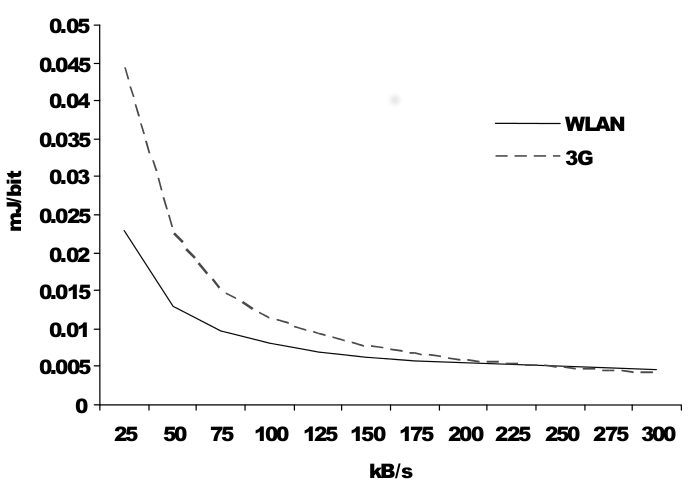
\includegraphics[scale=0.35]{Figures/energyConsumption.png}
 \caption{Consumo de energía por Bit de transferencia. WLAN vs 3G. Experimento realizado en celular Nokia N900 \cite{miettinen2010energy}}
 \label{fig:energyConsumption}
 \end{figure}

 
 Similarmente, una demora cuantiosa debido al ancho de banda de una red inalámbrica puede ser causante de un consumo de energía más alto, ya
 que la aplicación  se encuentra en estado inactivo a la espera del resultado.
 
 %%%%%%%%%%%%%%%%%%%%%%%%%%% OFFLOADING ALGORITHM %%%%%%%%%%%%%%%%%%%%%%%%%%%%%%%%%%%%5
 %%%%%%%%%%%%%%%%%%%%%%%%%%%%%%%%%%%%%%%%%%%%%%%%%%%%%%%%%%%%%%%%%%%%%%%%%%%%%%%%%%%%%%%%%%%%%%%%%%%%%%%%%%%%
 \section{Algoritmo de offloading }
\label{sec:offloadingAlgorithm}

En esta sección se presenta un algoritmo básico para la aplicación de \emph{offloading} de aplicaciones, el cual es representado 
en la Figura \ref{fig:offloadingAlgorithm}. Se debe resaltar que el algoritmo mostrado a continuación no es necesariamente  aplicado
en todos sistemas de \emph{offloading}.
El flujo comienza con la ejecución de la aplicación seguido por la revisión de los permisos del usuario para realizar \emph{offloading}. En caso posea estos privilegios, la aplicación revisa  si el servidor (sea 
de: red local o en la nube) está en conexión con el dispositivo móvil, revisando su conectividad. Posteriormente, se toma la decisión si realmente es viable y necesario el \emph{offloading}, cual sea el objetivo
principal: mejorar el rendimiento o ahorrar energía o ambos (descrito en la Sección
\ref{subsec:offloadingdecision}). Si la cuestión anterior es positiva, todo el entorno es favorable para su ejecución remota por lo que se migra el cálculo a servidores en la nube. En otro caso, la aplicación se ejecuta de manera local. 

El proceso \emph{offloading}, en especial la toma de decisión de \emph{offloading} es muy difícil de realizar con una adecuada precisión. 
Esto, debido a factores externos e internos del dispositivo móvil que fueron revisados en la Sección~\ref{sec:factors}.


 \begin{figure}[h]
   \centering
 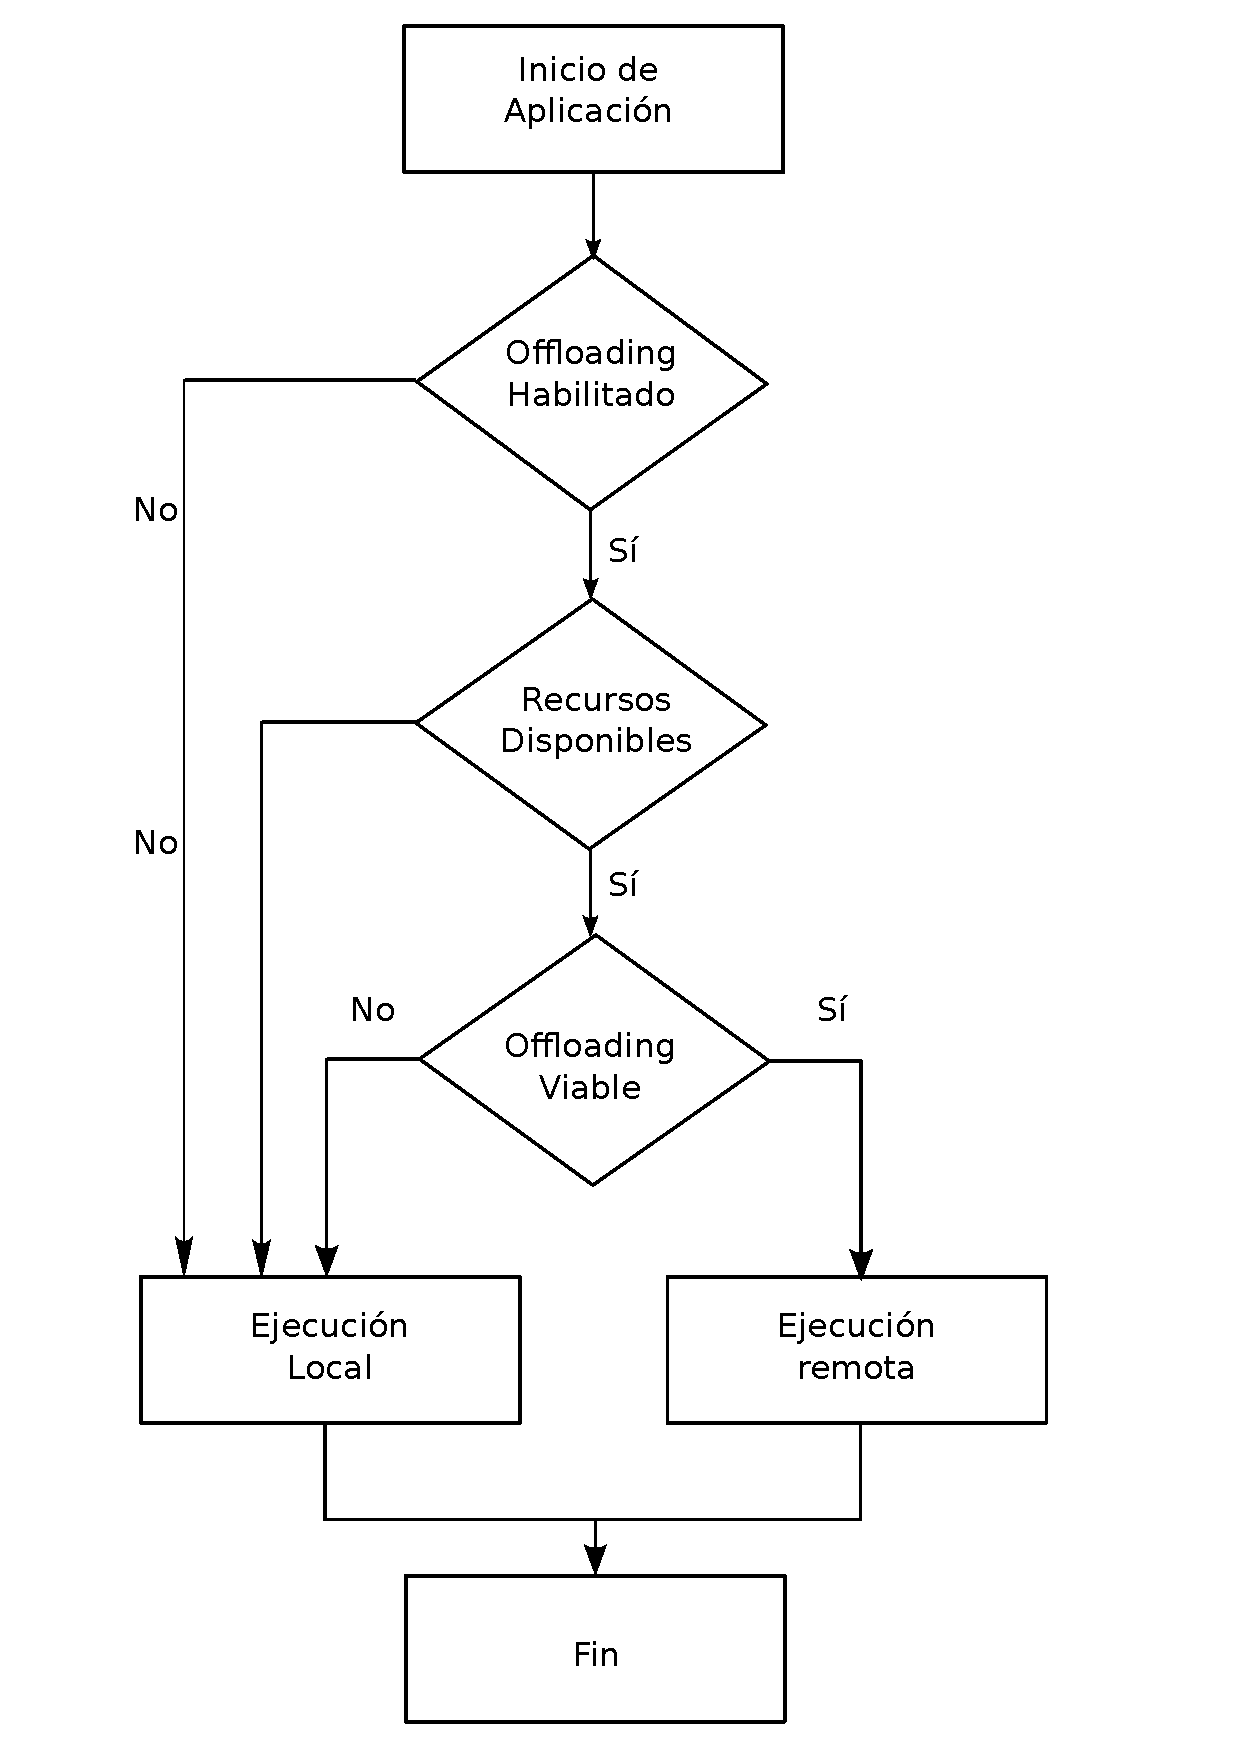
\includegraphics[scale=0.37]{Figures/processoffloadingcomputing}
 \caption{Proceso general de \emph{offloading}. Figura Adaptada de \cite{6553297} }
 \label{fig:offloadingAlgorithm}
 \end{figure}
 
 
 \section{Criterios para la clasificación de Offloading}
  \label{sec:metrics}
En las secciones anteriores fueron descritos los objetivos de la técnica de \emph{offloading} así como los factores que influyen en la toma de decisión para que ésta se realice. En este sección se describen los criterios de clasificación: tipo de \emph{offloading}, particionado de la aplicación y plataforma de despliegue. Posteriormente, se muestra una clasificación de los más importantes y actuales \emph{frameworks} de \emph{offloading} disponibles en MCC, la Tabla~\ref{table1:chart} muestra dicha clasificación siguendo los criterios anteriormente comentados.
 \begin{sidewaystable}
   %\begin{table*}[t]
 \footnotesize
 \caption{Algunas soluciones para el offloading de aplicaciones móviles}
 \begin{tabular}{lllllll}
\multicolumn{1}{c}{\cellcolor[HTML]{EFEFEF}{\color[HTML]{333333} \textbf{Año}}} & \multicolumn{1}{c}{\cellcolor[HTML]{EFEFEF}{\color[HTML]{333333} \textbf{Framework}}} & \multicolumn{1}{c}{\cellcolor[HTML]{EFEFEF}{\color[HTML]{333333} \textbf{Arquitectura}}} & \multicolumn{1}{c}{\cellcolor[HTML]{EFEFEF}{\color[HTML]{333333} \textbf{Objetivo Principal}}}            & \multicolumn{1}{c}{\cellcolor[HTML]{EFEFEF}{\color[HTML]{333333} \textbf{Tipo de Offloading}}} & \multicolumn{1}{c}{\cellcolor[HTML]{EFEFEF}{\color[HTML]{333333} \textbf{\begin{tabular}[c]{@{}c@{}}Plataforma \\ Cliente/Servidor\end{tabular}}}} & \multicolumn{1}{c}{\cellcolor[HTML]{EFEFEF}{\color[HTML]{333333} \textbf{\begin{tabular}[c]{@{}c@{}}Campo de \\ Aplicación\end{tabular}}}} \\
2002                                                                            & Spectra \cite{flinn2002balancing}                                                         & Orientado a Servicios                                                                    & \begin{tabular}[c]{@{}l@{}}Ahorro de Energía y reducción \\ de tiempo de Ejecución\end{tabular} & Estático                                                                                       & \begin{tabular}[c]{@{}l@{}}Entorno \\ Simulado\end{tabular}                                                                                        & \begin{tabular}[c]{@{}l@{}}Procesamiento\\ de Audio y \\ Documentos\end{tabular}                                     \\
2003                                                                            & Chroma \cite{balan2003tactics}                                                               & Orientado a Servicios                                                                    & Reducción de tiempo de Ejecución                                                                & Estático                                                                                       & \begin{tabular}[c]{@{}l@{}}Entorno\\ Simulado\end{tabular}                                                                                         & \begin{tabular}[c]{@{}l@{}}Procesamiento\\ de Imágenes\end{tabular}                                                  \\
2010                                                                            & MAUI \cite{Cuervo:2010:MMS:1814433.1814441}                                                  & Virtualización                                                                           & \begin{tabular}[c]{@{}l@{}}Ahorro de Energía \end{tabular}                    & Dinámico                                                                                       & \begin{tabular}[c]{@{}l@{}}Windows \\ Mobile / .Net\end{tabular}                                                                                   & \begin{tabular}[c]{@{}l@{}}Procesamiento\\ de Imágenes /\\ Juegos\end{tabular}                                       \\
2011                                                                            & CloneCloud \cite{chun2011clonecloud}                                                         & Virtualización                                                                           & \begin{tabular}[c]{@{}l@{}}Ahorro de Energía y reducción \\ de tiempo de Ejecución\end{tabular} & Dinámico                                                                                       & Android/Dalvik                                                                                                                                     & \begin{tabular}[c]{@{}l@{}}Análisis de Virus\\ /Búsqueda de \\ imágenes\end{tabular}                                 \\
2011                                                                            & COFA \cite{shivarudrappa2011cofa}                                                            & Orientado a Servicios                                                                    & \begin{tabular}[c]{@{}l@{}}Ahorro de Energía y reducción \\ de tiempo de Ejecución\end{tabular} & Estático                                                                                       & Android/Dalvik                                                                                                                                     & \begin{tabular}[c]{@{}l@{}}Cálculos\\  matemáticos\end{tabular}                                                      \\
2012                                                                            & COMET \cite{gordon2012comet}                                                                & Virtualización                                                                           & \begin{tabular}[c]{@{}l@{}}Reducción de tiempo de Ejecución \end{tabular}       & Dinámico                                                                                       & \begin{tabular}[c]{@{}l@{}}CyanogenMod\\ (Android)/Dalvik\end{tabular}                                                                             & \begin{tabular}[c]{@{}l@{}}Aplicaciones \\ Web\end{tabular}                                                          \\
2012                                                                            & Cuckoo \cite{kemp2012cuckoo}                                                                 & Orientado a Servicios                                                                    & \begin{tabular}[c]{@{}l@{}}Ahorro de Energía y reducción \\ de tiempo de Ejecución\end{tabular} & Estático                                                                                       & Android/JavaVM                                                                                                                                     & \begin{tabular}[c]{@{}l@{}}Juegos / \\ Procesamiento \\ de Imágenes\end{tabular}                                    
\end{tabular}
\label{table1:chart}
%\end{table*}
 \end{sidewaystable}
 \subsection{Particionado de la Aplicación}
 La presente investigación se basa principalmente en dos tipos de arquitecturas al momento de realizar el particionado:
 ``arquitecturas basadas en servicios'' y ``virtualización'' \cite{fernando2013mobile}.
 El primero es realizado entre el dispositivo móvil y el servidor vía protocolos como por ejemplo: llamadas a procedimiento remoto 
 (RPC, Remote Procedure Call), invocación de métodos remotos(RMI, Remote Method Invocation) y sockets.
 Dos ejemplos que utilizan estos protocolos son los \emph{frameworks} Chroma~\cite{balan2003tactics} y Spectra~\cite{flinn2002balancing}
 los cuales poseen pre-instalado en sus servidores servicios RPC para el proceso de \emph{offloading}. Otro ejemplo es el {\em framework 
 Cuckoo} ~\cite{kemp2012cuckoo}, \textit{framework} para
 \emph{offloading}  basado en Android OS\footnote{\url{http://developer.android.com/index.html}, último acceso en setiembre 2015}, como se observa en su arquitectura de la Figura ~\ref{fig:cuckoo}, utiliza interfaces
 para la comunicación con componentes
 nativos siguiendo el modelo {\em stub/proxy} en el lenguaje de programación Java. El {\em framework Cuckoo} utiliza el modelo por defecto 
 de Android {\em activity/service} que separa las actividades (métodos de interacción con el usuario) de los servicios
 (métodos de cómputo pesado).
 
\begin{figure}
\centering
  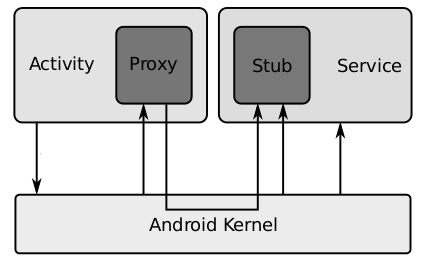
\includegraphics[scale=0.5]{Figures/cuckoo.png}
  \caption{Arquitectura del \emph{framework} Cuckoo \cite{kemp2012cuckoo}}
  \label{fig:cuckoo}
\end{figure}

 En el segundo tipo arquitectural, la virtualización, consiste en transferir la imagen de la memoria 
 de una máquina virtual (VM, \textit{Virtual Machine}) desde un servidor origen a un servidor destino sin detener su ejecución~\cite{clark2005live}. Durante la migración las páginas de memoria de la MV son copiadas previamente sin generar interrupción alguna en el sistema operativo, de tal modo que da la sensación de una migración natural. Una ventaja es que el código de la aplicación no necesita ser rescrito y provee una alta y segura ejecución, debido a que los límites de la MV lo aíslan. MAUI~\cite{Cuervo:2010:MMS:1814433.1814441} es \emph{framework} el cual usa una una mezcla de migración, entre MV y partición de código. Las aplicaciones que usan MAUI pueden transferir calculos a servidores tanto locales como remotos que estén sobre la infraestructura en la plataforma {\bf .NET}. Otro ejemplo es el \emph{framework} CloneCloud \cite{chun2011clonecloud} el cual usa migración de MV para transferir parte de la carga de la aplicación a servidores.
 
\subsection{Tipos de Offloading}

A fin de adaptar técnicas de \textit{offloading} en una aplicación, es concerniente al desarrollador conocer las posibles maneras para implementar,
así como sus posibles ventajas y desventajas. Tal adaptación puede ocurrir de dos maneras: de forma estática o dinámica~\cite{murarasu2009mobile}. En el primer enfoque el desarrollador define que
 secciones de código se ejecutarán remotamente. Esto ocurre en la fase de diseño o en la instalación y por 
 lo tanto cuando se inicia el ejecutable, el \emph{framework} conoce de antemano que partes del programa pueden ser
 enviados a ejecución remota. La 
 principal ventaja es que no existe una prominente sobrecarga en la aplicación, por tal motivo en este enfoque es necesario que los factores 
 que influyen en el algoritmo de decisión ( que describimos en la sección \ref{sec:factors}) sean predichos lo más exacto posible. Parámetros como
 poder de cálculo o ancho de banda en el lado del servidor son valores muy estables debido a que los grandes proveedores garantizan un nivel mínimo de 
 rendimiento.
 Algunos algoritmos de predicción de estos factores son: predicción basada en los registros históricos \cite{gurun2004nwslite} y predicción
 probabilística \cite{rong2003extending}. 
 Por otro lado, en el enfoque dinámico la ubicación de la parte a transferir no esta predeterminado por el desarrollador y tiene que 
 ser calculado generalmente en tiempo de ejecución, lo cual genera sobrecarga de cómputo. En este enfoque de igual manera existen mecanismos 
 de predicción para la toma de decisiones.Por ejemplo algunas propuestas construyen modelos de Markov como un modelo de movilidad (basados en
 el histórico de conexiones a puntos de acceso Wi-Fi), entonces es entrenado con patrones de movilidad del usuario \cite{lee2013user}. 
 En cambio, Wolski \cite{wolski2008using} en su investigación propone que el ancho de banda sea predicha usando un esquema bayesiano.
 

 \subsection{Plataforma de despliegue}
 
 Las soluciones para el \emph{offloading} de aplicaciones requieren desplegarse en plataformas móviles y en plataformas en nube. Para este motivo
 existe una pluralidad de plataformas heterogéneas en la computación en nube y en la computación móvil . 
 Esta heterogeneidad (como se observó en la Figura \ref{fig:heterogeinityRootsmcc} ) generalmente limita a los sistemas de
 \emph{offloading} a ejecutarse en todas las plataformas. Tal es el caso de 
 CloneCloud \cite{chun2011clonecloud} que explota el sistema operativo de código abierto AndroidOS
 para integrar su solución. Este sistema despliega una versión modificada de la máquina virtual de Dalvik (MV del sistema 
 Operativo Android) \cite{ehringer2010dalvik} en un servidor en la Nube con el fin de que acepte la transferencia de la aplicación.
 
 Otro ejemplo es el caso de MAUI \cite{Cuervo:2010:MMS:1814433.1814441}, el cual implementa una arquitectura basada en \emph{Windows Mobile}
 \footnote{\url{https://www.windowsphone.com/en-us}, último acceso en enero 2015}
 para su implementación  en el móvil, entre tanto que en el servidor  se despliega en un arquitectura \emph{.NET}. Cuckoo \cite{kemp2012cuckoo}
 por el lado del cliente está basado en Android, mientras que el servidor se ejecuta sobre la MV de Java. Este hecho hace posible que el 
 servidor de Cuckoo sea genérico y puede desplegarse sin mayor esfuerzo en cualquier tipo de servidor. En el caso de COMET \cite{gordon2012comet}
 en el lado del cliente se usa CyanogenMod \footnote{\url{http://www.cyanogenmod.org/}, último acceso en febrero 2015},
 una versión libre de Android mantenida por la Comunidad CyanogenMod.
 
 \subsection{Campo de Aplicación}
 
 Múltiples dominios pueden ser beneficiadas debido a la aplicación de \textit{offloading}. Para tal prueba del concepto, 
 los investigadores han 
 implementado aplicaciones sobre diferentes áreas. En esta sección presentamos ejemplos que demuestran el beneficio del empleo de 
 \textit{offloading}: 
 
 \begin{enumerate}
  \item Cálculos Matemáticos: Funciones matemáticas complejas, tal como la multiplicación de matrices de gran tamaño, o la 
  la secuencia de \textit{fibonacci} de un número considerable, esta última fue implementada por \textit{Shivarudrappa et al.} en su trabajo
  para aliviar carga computacional llamado COFA \cite{shivarudrappa2011cofa} 
  \item Procesamiento de Señales: Las tareas de procesamiento de señales como voz o imágenes demandan una alta carga computacional, y por ende 
  un consumo energético elevado. Por ejemplo, una aplicación de reconocimiento de patrones en imágenes como lo aplicaron los autores de MAUI 
  \cite{Cuervo:2010:MMS:1814433.1814441} en su caso de estudio, o en el caso de la aplicación \textit{eyeDentify}, la cual es 
  implementa usando el \textit{framework Cuckoo} \cite{kemp2012cuckoo} para el reconocimiento de objetos en imágenes. 
  \item Juegos: Las aplicaciones de juegos usualmente requieren un poder de cómputo pesado para mantener un renderizado suave de cada
  \textit{frame}, de tal manera
  que la interacción con el usuario sea rápida. En el trabajo propuesto por \textit{Kemp et al.} \cite{kemp2012cuckoo}, se presenta la aplicación
  \textit{PhotoShoot}, un juego multi-jugador de la categoría de disparos en primera persona (FPS, First Person Shooter) que sin la aplicación de 
  \textit{offloading}, a más lento el procesador del dispositivo móvil, más tiempo toma el disparo en ser analizado, lo cual da al usuario 
  con el móvil limitado una seria desventaja. Por ende, aplicar \textit{offloading} de cierto modo establece un juego más justo.
  \item Análisis de Virus: Estimando la creciente amenaza de virus y \textit{malwares}, las aplicaciones de la categoría antivirus están siendo
  una parte fundamental de los sistemas móviles. Sin embargo, el uso de dichos aplicativos demandan una gran cantidad de cálculo que consume
  una cantidad considerable de energía. El proceso de adaptar técnicas de \textit{offloading} en este dominio , podría aliviar estas limitaciones
  al realizar un escaneo 
  en la nube de una imagen del celular para ahorrar energía (asumiendo que el dispositivo móvil y su clon en la nube, están sincronizados). 
  Un ejemplo en esta área es el de \textit{CloneCloud} \cite{chun2011clonecloud}, el cual es usado para el caso de estudio de análisis de virus. 
  \cite{DBLP:journals/corr/abs-1105-3232}. 
  
 \end{enumerate}

 
  Similarmente, existe una variedad de aplicaciones que pueden tomar ventaja del uso de MCC. Sin embargo, aún existen aún retos abiertos consecuencia
  de su heterogeneidad presente.
 



























 
% Chapter 5

\chapter{Cloudlets} % Main chapter title

\label{ch:Chapter4} % For referencing the chapter elsewhere, use \ref{Chapter1} 

\lhead{Capítulo 4. \emph{Cloudlets}} % This is for the header on each page - perhaps a shortened title

%----------------------------------------------------------------------------------------

Con la ayuda de la nube, los dispositivos móviles pueden migrar las partes computacionalmente intensivas de sus aplicaciones. Los `inacabables' 
recursos de la nube pueden minimizar los costos de tiempo y energía de las aplicaciones móviles. Sin embargo, como se describió en la sección
\ref{ch:Chapter4}, uno de los aspectos que interfieren realizar \textit{offloading} a la nube es la alta latencia entre la conexión entre el móvil 
y la nube. Adicionando un cloudlet ~\cite{5280678} (una computadora local que provee de 100 a 1000 veces más poder computacional que un dispositivo móvil con 
mínima latencia), crea las posibilidades para ejecutar aplicaciones sensibles a la latencia y que demanden gran poder computacional de un dispositivo
móvil. La noción de \textit{cloudlet} fue introducida como solución a los obstáculos técnicos descritos anteriormente. La idea 
principal es proveer recursos abundantes que son necesitados por los dispositivos móviles no desde una \textit{nube} distante, sino desde
un \textit{cloudlet} cercano. Satyanarayanan \textit{et al.} resumió las diferencias entre \textit{cloudlet} y \textit{cloud}, las cuales están
listadas en la tabla \ref{tab:mainDifferencescloudletcloud}. Se debe notar que el estado flexible sugiere que las copias de cache, datos 
o código están en el dispositivo móvil o \textit{cloud}. En tanto, el estado rígido se refiere a que existe solo una única copia de 
datos o código. Debido a que el \textit{cloudlet} tiene estado flexible, la pérdida de un \textit{cloudlet} no es algo grave. 

%mccarchitecturevscloudlet
% Please add the following required packages to your document preamble:
% \usepackage[table,xcdraw]{xcolor}
% If you use beamer only pass "xcolor=table" option, i.e. \documentclass[xcolor=table]{beamer}
\begin{table}[]
\centering
\caption{Diferencias más notorias entre los entornos \textit{cloudlet} y \textit{cloud} \cite{5280678}}
\label{tab:mainDifferencescloudletcloud}
\begin{tabular}{|l|l|l|}
\hline
\rowcolor[HTML]{EFEFEF} 
               & \multicolumn{1}{c|}{\cellcolor[HTML]{EFEFEF}{\bf Cloudlet}}                                   & \multicolumn{1}{c|}{\cellcolor[HTML]{EFEFEF}{\bf Cloud}}                                                     \\ \hline
Estado         & Solo estado flexible                                                                          & Estado flexible y  rígido                                                                                    \\ \hline
Administración & \begin{tabular}[c]{@{}l@{}}Autogestionado, poca o sin\\  atención profesional\end{tabular}    & Administrado profesionalmente 24/7                                                                           \\ \hline
Entorno        & \begin{tabular}[c]{@{}l@{}}Propiedad descentralizada por \\ los negocios locales\end{tabular} & \begin{tabular}[c]{@{}l@{}}Propiedad centralizada por \\ pocas Empresas (Amazon, Google, etc. )\end{tabular} \\ \hline
Red            & \begin{tabular}[c]{@{}l@{}}Latencia dependiente de la \\ Red de Área Local (LAN)\end{tabular} & \begin{tabular}[c]{@{}l@{}}Latencia de Internet o Ancho de \\ Banda\end{tabular}                             \\ \hline
Escalamiento   & Pocos usuarios a la vez                                                                       & Cientos, Miles o Millones de usuarios a la vez                                                               \\ \hline
\end{tabular}
\end{table}

\subsection{Arquitectura Cloudlet}

Como se describió anteriormente, los \textit{cloudlets} pueden ser usados como intermediarios entre los dispositivos móviles y los servidores 
en la \textit{nube}. Una de las primeras implementaciones de una arquitectura \textit{cloudlet} fue un prototipo de sistema de computación
cloudlet llamado Kimberley~\cite{5280678}, desarrollado por Satyanarayanan \textit{et al.}.  En contraste con la arquitectura en nube, 
Kimberley está conectado a los móviles a través de LAN, no WAN, y es accedido por solamente unos usuarios a la vez. En la Figura
~\ref{fig:mccarchitecturevscloudlet} se 
muestra la arquitectura \textit{cloudlet} en comparación con la arquitectura en nube. El rol principal que cumple un \textit{cloudlet} 
es la administración de tareas. También puede colaborar al dispositivo móvil con algún tipo de procesamiento intermedio.

La arquitectura MOCHA \cite{soyata2013accelerating} (Mobile CLoud Hybryd Architecture) fue creada como una solución a aplicaciones de nube para móviles que requieren
una masiva cantidad de tareas paralelizables. Dicha arquitectura permite que laptops, touchpads, y smartphones se connecten a la nube 
via \textit{cloudlets}, este servicio se realiza usando conexiones de redes múltiples como 3G/4G, Bluetooth, y WiFi. El \textit{cloudlet}
determina como dividir el cálculo entre si mismo y múltiples servidores para optimizar la calidad de servicio (QoS, Quality of Service) 
basado en modelos estadísticos de métricas QoS (latencia, costo monetario, poder de procesamiento, etc.). MOCHA fue demostrado usando 
tareas de reconocimiento de rostros. 
Una arquitectura Similar a Kimberly y a MOCHA, fue propuesta por Ha \textit{et al.}. Esta arquitectura de dos niveles aprovecha un nivel 
de infraestructura en la nube, y un segundo nivel en el borde o \textit{edge} del internet, sirviendo a los dispositivos móviles incorporados 
a la red por medio de WiFi. Los \textit{cloudlets} son pequeños centros de datos próximos al usuario, los cuales solo 
tienen estados flexibles guardados en caché de la nube o de los dispositivos móviles. 
En algunos escenarios como una construcción de oficina, múltiples \textit{cloudlets} pueden estar localizados cerca a otros y pueden estar 
conectados de una forma punto-a-punto. En este caso, la ruta entre entre los móviles, servidores en nube, y los \textit{cloudlets} tiene
que ser tomada en cuenta. En la investigación de Fesehaye \textit{et al.} \cite{6337243} fueron propuestos dos tipos de esquemas de 
enrutamiento o \textit{routing}: centralizado y descentralizado. En el enrutamiento descentralizado la tabla de enrutamiento está 
construida y mantenida por los \textit{cloudlets}. Los \textit{cloudlets} periódicamente emiten información de su presencia a los nodos
vecinos y los otros \textit{cloudlets}. Cuando un dispositivo móvil recibe un mensaje \textit{broadcast} desde un \textit{cloudlet}, 
almacena tal información en una tabla de \textit{cloudlets} adjunto a un identificador (ID) del \textit{cloudlet}. Cada móvil también emite 
periódicamente un mensaje tipo \textit{broadcast} con su identificador, de tal forma que todos los \textit{cloudlets} tengan conocimiento. En 
el enrutamiento centralizado el servidor central es responsable de preparar y mantener la tabla de rutas. El \textit{cloudlet} periódicamente
envía su ID, los ID de sus usuarios móviles y los ID de los \textit{cloudlets} vecinos al servidor central. Consecuentemente, el
servidor central calcula la tabla de rutas para cada \textit{cloudlet} e instala la tabla de reenvíos en todos los \textit{cloudlets}.
\begin{figure}[h]
  \centering
 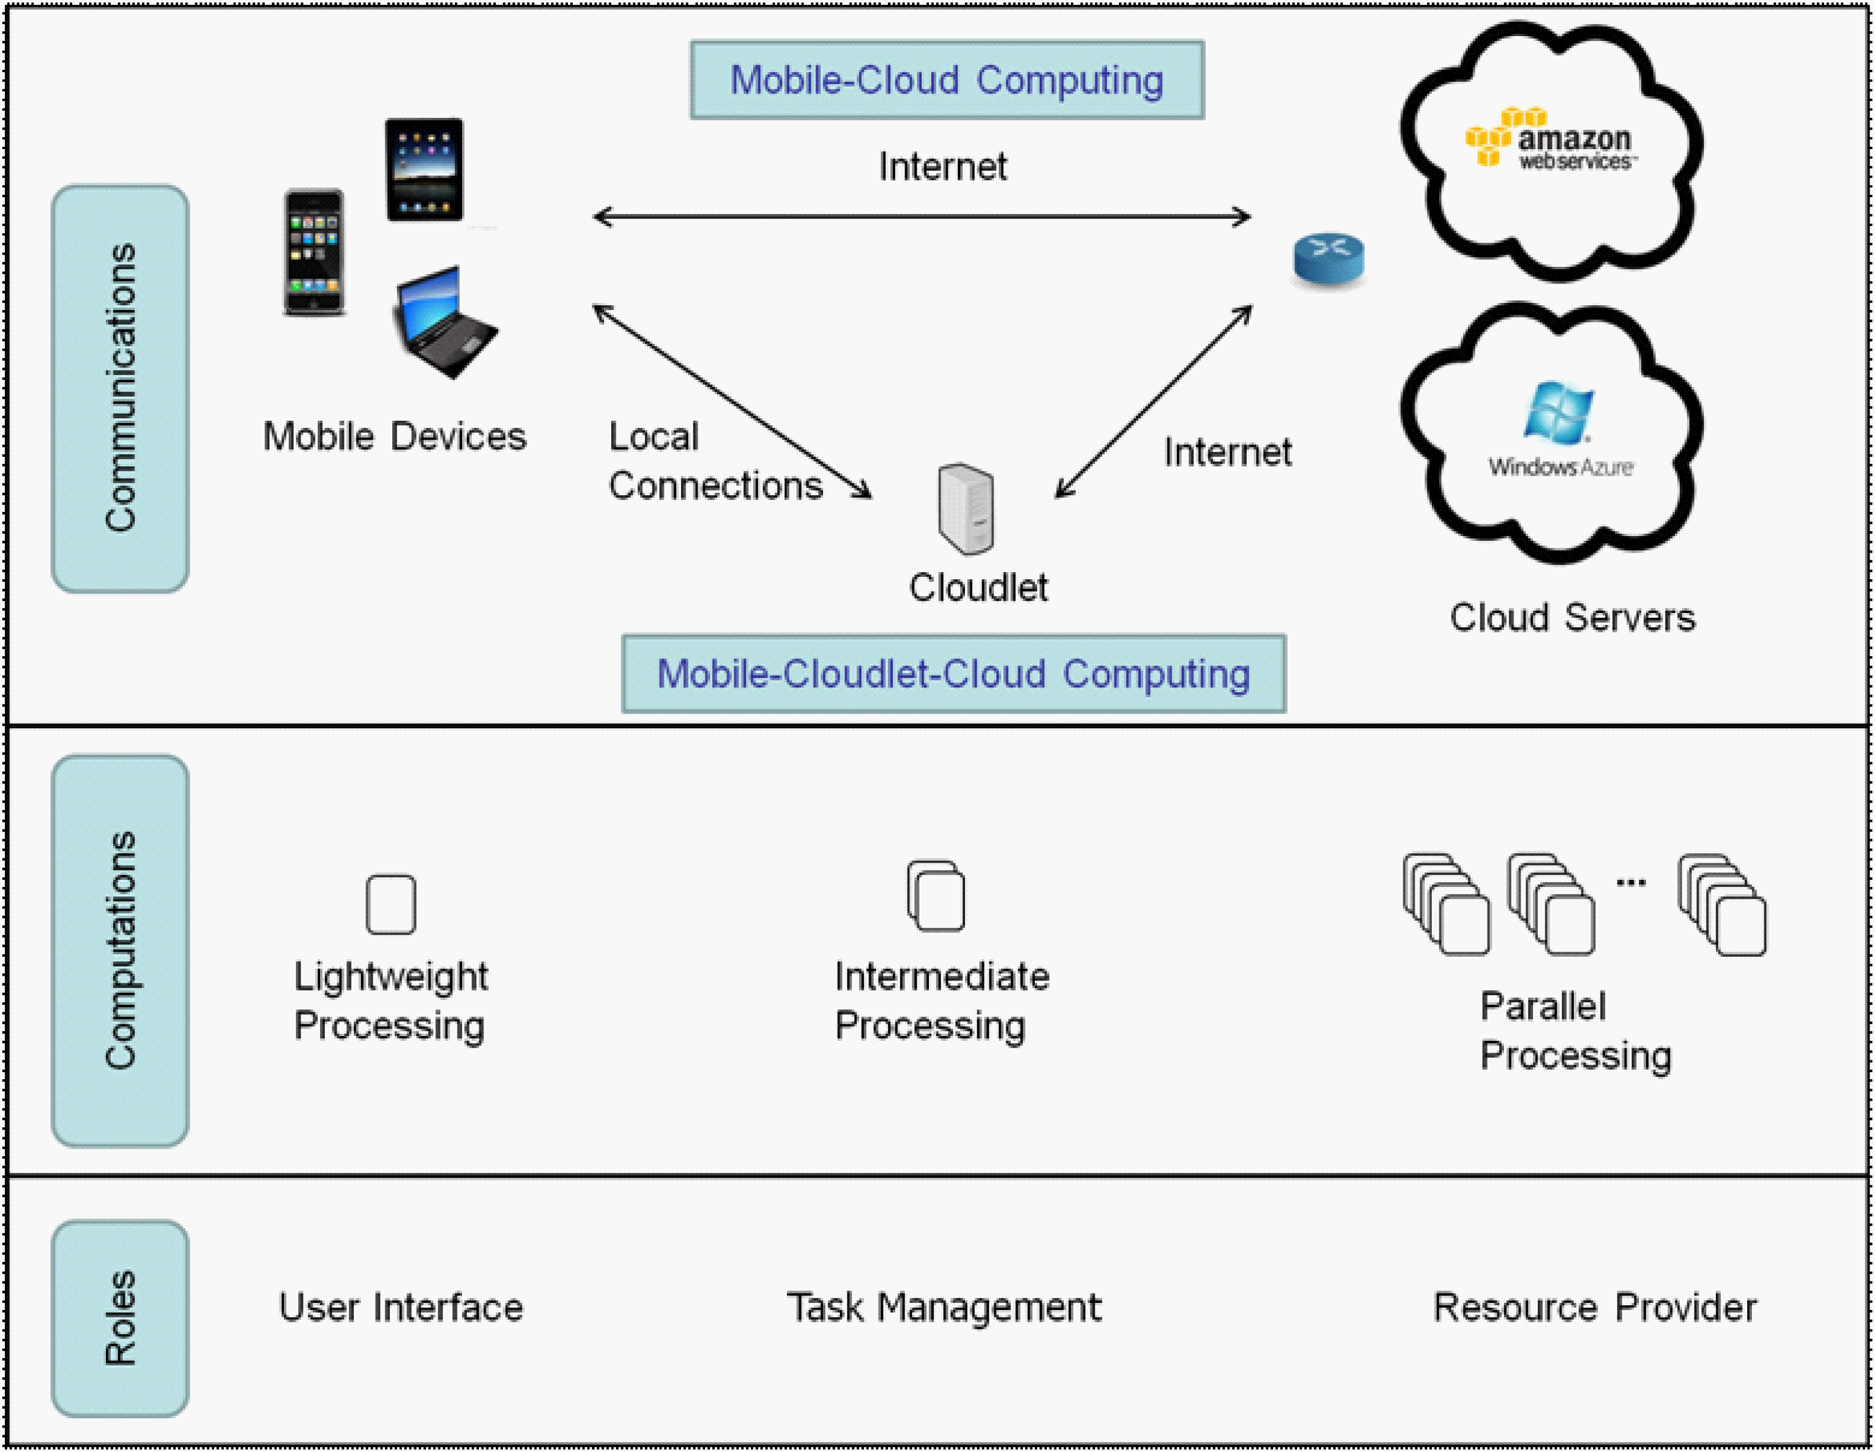
\includegraphics[scale=0.20]{Figures/mccarchitecturevscloudlet}
 \centering \caption{Diferencias entre las arquitecturas basadas en nube y las basadas en cloudlet \cite{soyata2013accelerating}}
 \label{fig:mccarchitecturevscloudlet}
\end{figure}


% Chapter 6

\chapter{Propuesta: Sistema Pytos} % Main chapter title

\label{ch:Chapter5} % For referencing the chapter elsewhere, use \ref{Chapter1} 

\lhead{Capítulo 5. \emph{Arquitectura de Pytos}} % This is for the header on each page - perhaps a shortened title

%----------------------------------------------------------------------------------------

En este capítulo son descritos los niveles jerárquicos involucrados en la Arquitectura de Pytos, a fin de realizar cómputo al borde de la red y 
optimizar los recursos móviles. 

\section{Arquitectura de Pytos}
\label{sec:pytosSystem}
Pytos es un \textit{framework} basado en Python que será implementado sobre un entorno \textit{cloudlet} con soporte de la nube. 
En la figura \ref{fig:pytosOverview} se muestran los componentes de Pytos desplegados sobre tres capas jerárquicas: (i) dispositivo cliente, 
(ii) \textit{cloudlet} y (iii) servidor 
en nube. La arquitectura propuesta cuenta con un componente privado, el cual es alojado y administrado en servidores de nuestro grupo 
de investigación. 
Este componente da soporte en el proceso de
descubrimiento de \emph{cloudlets} disponibles en una determinada red de área local. Los propósitos principales de que los servidores 
de consulta de \emph{cloudlets}
sean centralizados, en nube y administrados por Pytos; son: (i) seguridad, los programadores que usan Pytos pueden confiar su código en los cloudlets 
certificados por Pytos, (ii) disponibilidad, los \emph{cloudlet} disponibles en una red son consultados al servidor central de Pytos usando 
Internet desde cualquier lugar, y iii) facilidad, el desarrollador no se preocupa en instalar o desplegar el componente \emph{cloudlet}
. Entonces, el procedimiento mencionado de \emph{offloading} será realizado de forma transparente al usuario final y 
con facilidad para el desarrollador. Además de los beneficios en ahorro de energía y tiempo de respuesta en los móviles, consideramos 
una contribución importante la migración de tareas con envío a la nube, la cual se muestra en la parte a) de la Figura \ref{fig:pytosOverview}. 
A diferencia de la migración de tareas con data de retorno (donde las aplicaciones cliente están a la espera de un resultado desde el cloudlet
imagen b) de la Figura~\ref{fig:pytosOverview}), las aplicaciones con envío directo a nube entregan los resultados a una aplicación en nube 
especificada por el programador. Este modelo es útil cuando se realiza un pre-procesamiento antes de realizar \emph{streaming} de datos sin
necesidad
de volver al dispositivo móvil (codificación de video y audio, procesado de imágenes en tiempo real, etc.). En el caso no esté disponible   

%Esta arquitectura propuesta permite a las aplicaciones aliviar las limitaciones de los recursos móviles al migrar las tareas que 
%requieren un
%cálculo intensivo al \textit{cloudlet}. 


%desarrollador. El servidor de la nube de Pytos contiene un
%repositorio de \textit{cloudlets} disponibles por ubicación. Por lo tanto, se da libertad a los clientes consultar por el \textit{cloudlet}
%más cercano actualmente anexo a la red WLAN, a través de un proceso de descubrimiento de \textit{cloudlets}. Después de que Pytos es desplegado
%sobre los 3 niveles jerárquicos, Pytos decide si es ventajoso realizar \textit{offloading} al \textit{cloudlet} o no. 

El principal objetivo de la arquitectura propuesta es mejorar el rendimiento de los servicios basados en \textit{cloudlets} en lugares públicos 
de gran afluencia, como hospitales, restaurantes, cafetería o centros comerciales. Además, a través de la localización de \textit{cloudlets}, el 
framework puede facilitar y mejorar el rendimiento de aplicaciones que demanden gran cantidad de recursos, sensibles a la demora, trayendo los
recursos de la nube más cerca al usuario final.

\begin{figure}
\centering
 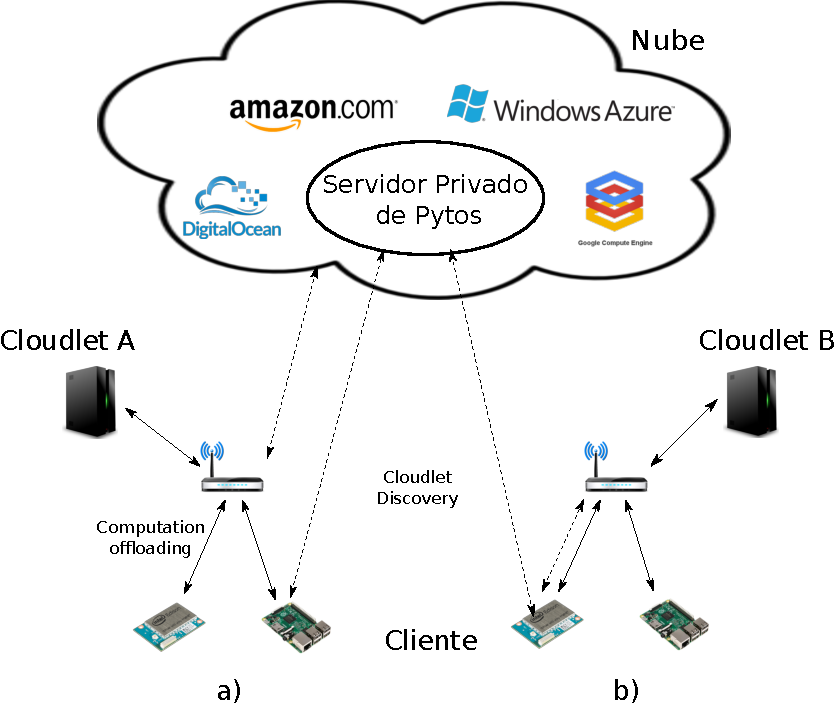
\includegraphics[scale=0.72]{Figures/generalArchitecture.pdf}
 \caption{Vista global de la arquitectura propuesta de Pytos}
 \label{fig:pytosOverview}
\end{figure}

Se propone un entorno de programación donde los desarrolladores seleccionen los métodos deseados de una aplicación que podrían ser migrados para
su ejecución remota. Cada vez que un método sea invocado y el servidor remoto esté disponible, Pytos usará su framework de optimización para decidir 
si el método debe ser migrado en tiempo de ejecución.
Con el objetivo de maximizar los beneficios de la infraestructura \textit{cloudlet}, se considera los siguientes componentes (ilustrados en la 
figura \ref{fig:pytosArchitecture}) : 

\begin{enumerate}
 \item \textbf{Biblioteca de Pytos:} Este componente provee la sintaxis para usar los decoradores de Pytos (descrito en la sección~\ref{sec:programmingModel}), el cual es precisado para interceptar
 el método de cómputo elevado. Además, inicializará un proceso demonio \textit{Pytos Daemon} si no ha sido inicializado uno anteriormente.
 \item \textbf{Pytos Daemon:} Es el componente fundamental del sistema de Pytos, el cual es compuesto de tres módulos principalmente:
 \begin{itemize}
\item El recopilador, que recauda información del contexto del móvil como: el estado de la red inalámbrica y el tiempo de ejecución en el servidor 
y el \textit{cloudlet}. Seguidamente, los valores del recopilador son enviados a la función de costo;
\item El evaluador o planificador de tareas, es responsable de evaluar la función de costo, ya que toma la decisión de \textit{offloading} más adecuada; y 
\item El explorador,  destinado a buscar nuevos \textit{cloudlets} disponibles. Como fue discutido anteriormente, este módulo consulta el repositorio
de \textit{cloudlets} de la aplicación localizados en el servidor en nube. 

\end{itemize}
 \item \textbf{Modelo de predicción:} En este componente se aborda el medio para optimizar la decisión de \textit{offloading}. En esta escena,
 un modelo probabilístico de regresión lineal es implementado para pronosticar el tiempo de ejecución de un método migrado al lado del
 \textit{cloudlet}. Entonces, los valores estimados son retornados al evaluador como una entrada en la función de costo.
 \item \textbf{\textit{Endpoints}\footnote{\url{https://cloud.google.com/appengine/docs/java/endpoints/}, Último acceso en setiembre 2015} de descubrimiento:} Ubicados en el componente \textit{cloudlet} donde una Interface de entrada en un Servidor
 Web (Web Server Gateway Interface, WSGI) \footnote{\url{https://www.python.org/dev/peps/pep-0333/}, último acceso en junio 2015} se ejecuta con la intención de dar soporte al cliente en el proceso de descubrimiento
 de \textit{cloudlets}. Se aprovecha el recurso centralizado en la nube para almacenar un repositorio general de \textit{cloudlets}.
 \item \textbf{Contenedor Pytos:} En este componente se ejecutará la tarea migrada de la aplicación. La función decorada definida 
 en el 
 código de programa inicial es convertida a \textit{endpoints} abiertos y accesible con un token de autorización basado en el modelo 
 distribuido REST. Los resultados son enviados nuevamente al cliente, o enviados directamente a la aplicación en nube especificada por el 
 desarrollador. Cada tarea migrada al poseer un \emph{token} único se podrá almacenar y utilizar nuevamente si es requerida por un periodo de tiempo.
 Los \textit{endpoints} son declarados usando un Identificador de Recurso Único (URI, Uniform Resource Identifier)~\cite{Walsh_architectureof}.
 \item \textbf{Aplicación web del Desarrollador:} Este componente es opcional. Si el desarrollador lo determinó en su aplicación cliente, el resultado 
 será enviado desde el contenedor Pytos hasta el servidor definido por el desarrollador. Por ejemplo, puede ser implementado un juego cooperativo 
 de realidad aumentada, el cual requiera procesar a cada frame de video antes de ser enviado a Internet. Creemos que tal proceso aliviaría 
 el costo operacional de los servidores en nube, delegando la tarea pesado de procesamiento de los frames a los \emph{cloudlets}. 
 
\end{enumerate}
En las secciones siguientes se describen los componentes indicados anteriormente en mayor detalle.

\begin{figure}
\centering
 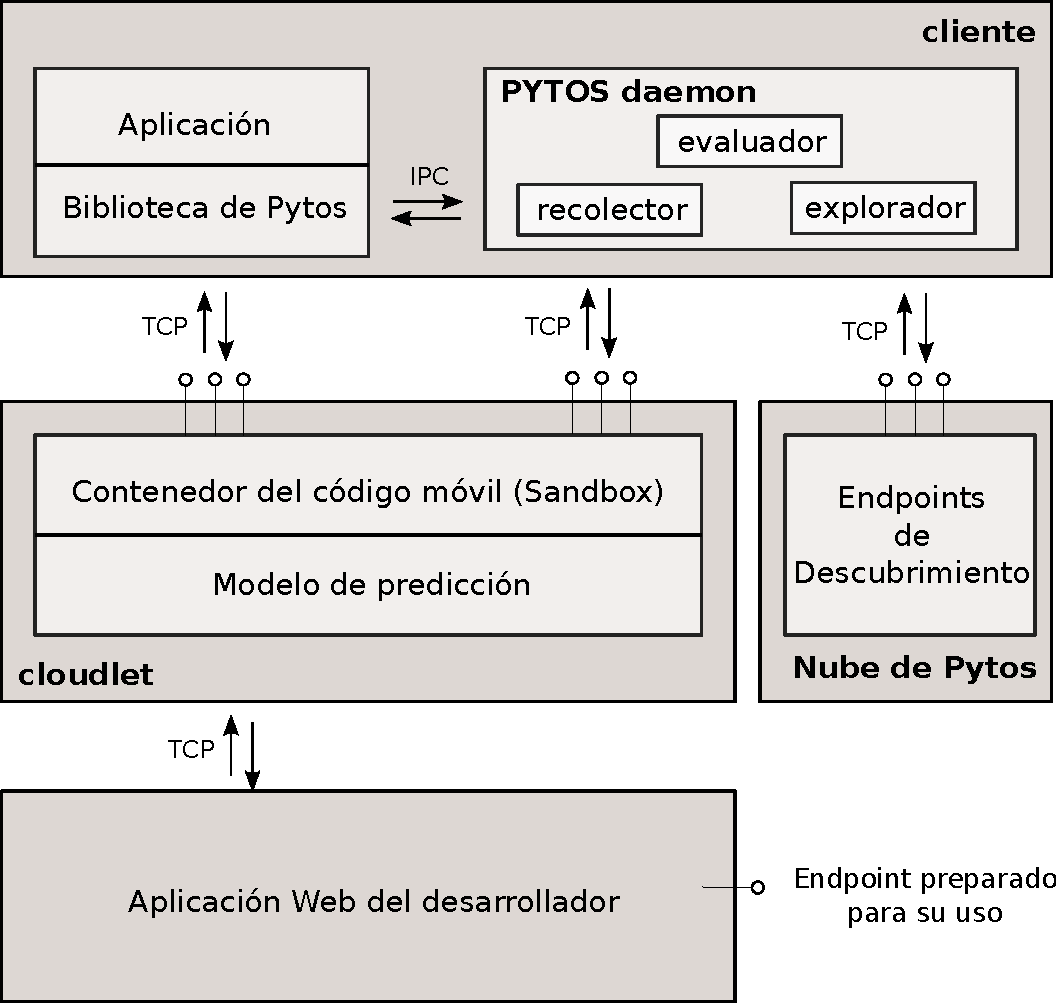
\includegraphics[scale=0.55]{Figures/components.pdf}
 \caption{Detalles de interacción entre los componentes de Pytos}
 \label{fig:pytosArchitecture}
\end{figure}


%%%%%%%%%%%%%%%%%%%%%%%%%%%%%%%%%%%%%%%%%%%%%%%%%%%%%%%%%%%%%%%%%%%%%%%%%%%%%%%%%%%%%%%%%%%%%%%%%%%%%%%
\section{Diseño de Pytos}
\label{sec:pytosDesign}
Después de la introducción inicial de las ventajas de migración de cómputo en el capítulo  \ref{ch:Chapter4} como una técnica para mejorar 
el rendimiento y reducir el uso de la batería en aplicaciones con cálculos intensivos; en esta sección son descritos los detalles de diseño
sobre la adición de la técnica de \textit{offloading} a una aplicación de una manera simple sin un esfuerzo adicional. Nuestro enfoque
tiene como objetivo la simplicidad, considerando:

\begin{enumerate}
 \item El uso de Python \footnote{\url{https://www.python.org/}, último acceso en junio 2015}, este lenguaje de programación de alto nivel es ampliamente usado para propósitos generales y tiene 
 una gran variedad de bibliotecas, las cuales en su gran mayoría son actualizadas periódicamente. 
 \item El uso de los \textit{decoradores} de Python \footnote{\url{https://www.python.org/dev/peps/pep-0318/}, último acceso en junio 2015}, 
 pues permite la selección a nivel de métodos. Tal cualidad permite 
 a los desarrolladores agregar \textit{offloading} de una manera sencilla.
 \item El proceso de descubrimiento de \textit{cloudlets} simple y transparente al usuario final
\end{enumerate}

\section{Modelo de Programación}
\label{sec:programmingModel}
Python tiene un modelo de programación potente, con características avanzadas y sintaxis expresiva. Uno de ellos son los \textit{decoradores},
los cuales generalmente son usados para alterar dinámicamente la funcionalidad de un método sin tener que usar directamente el uso de subclases. 
Esta característica encaja adecuadamente en nuestro enfoque para extender la funcionalidad de un método que \textit{puede} ser migrado fácilmente.
En el código \ref{list:pytosSample} se ilustra como un método es \textit{decorado} con la sintaxis de Pytos. Por lo tanto, el motor de Pytos podrá 
decidir en tiempo de ejecución si el \textit{offloading} es ventajoso o no.
%\vspace{0.5cm}

\begin{lstlisting}[caption= Ejemplo del uso de la sintaxis de Pytos sobre un método que \textit{puede} ser migrado, label=list:pytosSample]
@offload
def faceRecognition(self,img):
    faces = faceCascade.detectMultiScale(img,CTE1, CTE2)
    return faces
\end{lstlisting}

\vspace{0.5cm}
Luego que las funciones son seleccionadas, lo que el motor de Pytos hace es : 1) interceptará el código del método, 2) generar un código único o
\emph{token} que identifique al método, 3) encolar la tarea en el planificador inmediatamente, 4) revisar si es viable el envío de código al 
\emph{cloudlet}. 5) instalar el código de la función en el \emph{cloudlet} si es necesario, 6) ejecutar la tarea (local o remotamente) y esperar por 
el resultado (si no existe soporte de la nube). Las funciones \textit{decoradas} serán convertidas en puntos de salida HTTP
o \textit{endpoints} de la aplicación en el \textit{cloudlet} con identificadores URIs \footnote{\url{http://www.ltg.ed.ac.uk/~ht/WhatAreURIs/}}.


\subsection{Flujo del Sistema}
\label{sec:pytosWorkflow}
Nuestra propuesta de framework llevará a las aplicaciones móviles basadas en \textit{cloudlets} por los siguientes pasos antes de realziar la migración
de computación al \textit{cloudlet}. En la Figura ~\ref{fig:pytosWorkflow} se muestra el proceso de \textit{offloading} de cómputo.

\begin{enumerate}
 \item \textit{Proceso de descubrimiento de \textit{cloudlets}}: En esta fase, el explorador de Pytos solicita los \textit{cloudlets} disponibles
 en un red. Esta demanda toma el Identificador de Conjunto de Servicio\footnote{\url{http://www.webopedia.com/TERM/S/SSID.html}} (SSID, Service 
 Set Identifier) de la red WLAN que esté conectada en el momento como un parámetro de entrada.
 \item \textit{Decisión de \textit{offloading}:} Consecuentemente, en el siguiente paso es realizada la decisión inteligente de \textit{offloading}.
 En el cual el objetivo de Pytos es optimizar el rendimiento, por lo que el ancho de banda de la red y los tiempos de ejecución son 
 recolectados y transferidos a la función de evaluación (discutido en la sección~\ref{sec:intelligentOffloading})
 \item \textit{Ejecución de tareas pesadas}: La función de cómputo intensivo es ejecutada. Si es ejecutada remotamente, los parámetros del método
 y respuestas son colocados en una archivo con notación de Objeto JavaScript \footnote{\url{http://json.org/}, último acceso en febrero 2015}
 (JSON, JavaScript Object Notation). Entonces, estos datos
 livianos con enviados sobre la capa de transporte TCP.
\end{enumerate}

\begin{figure}
\centering
 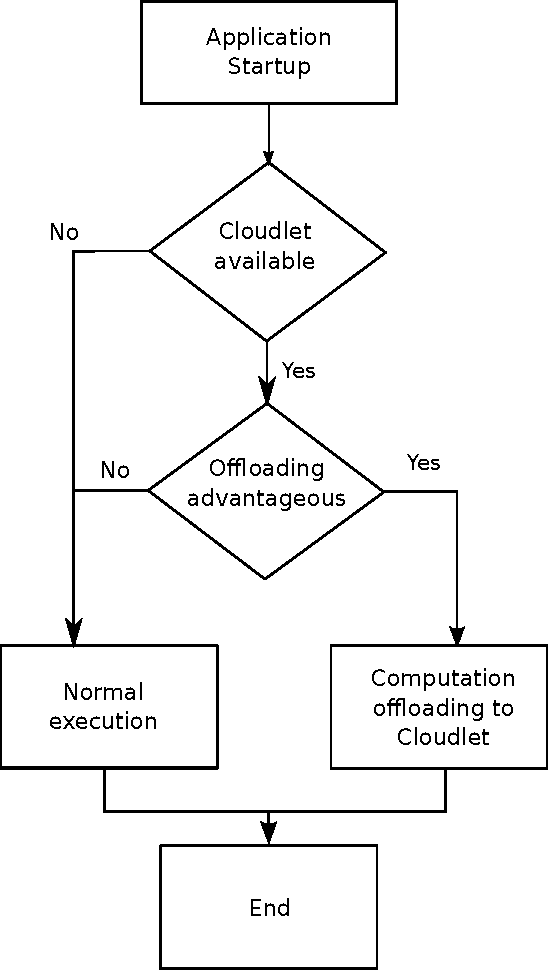
\includegraphics[scale=0.6]{Figures/pytosworkflow.pdf}
 \caption{Flujo del sistema de Pytos}
 \label{fig:pytosWorkflow}
\end{figure}


\section{Implementation}
\label{sec:implementation}

En esta sección resaltamos los detalles de implementación del framework Pytos. Se describe como el recopilador de red recolecta la información 
relevante del contexto móvil con el objetivo de realizar un \textit{offloading} inteligente antes de enviar el cómputo al \textit{cloudlet}. 
Finalmente, explicamos como el costo de evaluación es realizado priorizando el aspecto del rendimiento. 

%Finally, we show the architecture
%details of the components involved in our framework. 

\subsection{Recopilador}

Como mencionamos anteriormente, Pytos será capaz de realizar una decisión de \textit{offloading} inteligente en tiempo de ejecución: si la 
ejecución de la función debe ejecutarse remotamente o localmente. Para alcanzar tal objetivo, se implementará un recopilador a fin de recolectar
toda la información importante del contexto móvil, como: 1) características de la Red WLAN (ratio de transferencia, latencia) y 2) características
del contexto de la aplicación relacionadas al tiempo de ejecución en el \textit{cloudlet} y localmente (dispositivo móvil).

Para reunir el estado de la red, nosotros consideramos la técnica usada por Cuervo {\em et. al.}~\cite{Cuervo:2010:MMS:1814433.1814441}. Se 
implementará un proceso demonio de Pytos para enviar un paquete de 10kb al cloudlet a fin de medir el tiempo de transferencia. Usando este simple
enfoque permite que el recolector de Pytos obtenga los valores estimados de la latencia y ancho de banda. Tal procedimiento es realizado cada tres 
minutos para mantener un valor estimado actualizado. 
Similarmente, el proceso demonio de Pytos consulta el \textit{cloudlet} por información estadística basados en históricos sobre las funciones de 
cómputo pesado que fueron realizadas en el pasado. Luego, tales valores (1) y (2) son enviados a la función de costo (discutido en la Sección 
~\ref{sec:intelligentOffloading})

\subsection{Evaluador}
\label{sec:intelligentOffloading}
%The Pytos solver performs the cost function evaluation, using the information collected by Pytos profiler. 

Nuestra investigación se centra en minimizar el tiempo de ejecución de una función de cómputo pesado. En tal sentido, se construirá una función
de evaluación que considere lo siguiente: tiempo de ejecución en el \textit{cloudlet} y en el cliente, además del tiempo de transferencia. 
Estos valores son obtenidos del componente recopilador de Pytos. Usaremos la ecuación~\ref{eq:executiontimeFinal} explicada en la sección 
\ref{ch:Chapter4} como función evaluadora. 


%%%%%%%%%%%%%%%%%%%%%%%%%%%%%%%%%%%%%%%%%%%%%%%%%%%%%%%%%%%%%%%%%%%%%%%%%%%%%%%%%%%%%%%%%%%%%%%%%%%%%%%
\section{Resultados Iniciales}
\label{sec:evaluation}
En esta sección describimos la configuración experimental adoptada para evaluar la migración de tareas en un entorno \textit{cloudlet}. 
Dicho experimento en que factor el \textit{offloading} de cómputo es posible ahorrar energía y mejorar el rendimiento. Por lo que, se implementó
una aplicación de reconocimiento de rostros usando \textit{offloading} y fue probado sobre un conjunto de imágenes.


\subsection{Configuración experimental}

Con el objetivo de demostrar las ventajas del \textit{offloading} en un entorno \textit{cloudlet}, se consideraron los componentes de una 
jerarquía de tres niveles: cliente, \textit{cloudlet} y nube.

En el cliente, se utilizó una mini-computadora Intel Edison que incorpora la placa de expansión de Arduino 
\footnote{\url{https://www-ssl.intel.com/content/www/us/en/do-it-yourself/edison.html}, Último acceso en setiembre 2015} para direccionar la 
conexión con interfaces de Entrada/Salida externas como dispositivos de cámara web USB, tarjeta de expansión de memoria micro SD y entrada 
de energía. Esta placa incorpora un CPU Intel Atom con una frecuencia de 500 MHz de doble núcleo, 1 GB de memoria RAM y una antena WiFi 
interna IEEE 802.11a/b/g/n. 

Se usó como sistema operativo Ubilinux \footnote{\url{http://www.emutexlabs.com/ubilinux}, último acceso en setiembre 2015} 
de la distribución Debian (versión 150309). En el \textit{cloudlet} se utilizó una computadora de escritorio equipada con un CPU Intel Core i7-4700MQ
a una frecuencia de 2.40 GHz, 11.5 GiB de memoria RAM, y Ubuntu 14.04 como sistema operativo. En el servidor en nube se dispuso de una máquina 
virtual con Ubuntu 14.04 (7 núcleosy 16 GiB de memoria RAM), el cual pertenece a la empresa Digital Ocean~
\footnote{\url{https://www.digitalocean.com/}, último acceso en setiembre 2015} y está físicamente localizado en New York. 
Durante los ensayos, el ancho de banda de la conexión entre el cliente y el \textit{cloudlet}, medido con la herramienta Iperf benchmar 
\footnote{(\url{https://iperf.fr/}, último acceso en setiembre 2015}, fue aproximadamente 8.90 Mbits/seg. 
Todas las conexiones fueron realizadas sobre el protocolo TCP, usando un Punto de Acceso provisto por TP-link, en su modelo Archer C2.
Para obtener medidas de energía a grano fino, se consideró el uso de la herramienta PowerAPI~\cite{bourdon2013powerapi}, una biblioteca de 
software para monitorear la energía consumida a nivel de procesos. Dicha herramienta, nos permite conseguir de manera estándar y con alta precisión
(similar a los multímetros convencionales) las unidades \textit{watt} consumidas por el proceso deseado. Relegamos el consumo de energía realizado
por la interfase de WiFi, ya que este valor es dominado por el consumo de energía del CPU \cite{chen2015smartphone}. 

La metodología usada para obtener la energía y tiempo de respuesta se muestra en la Figura \ref{fig:experimentalSetup}. En tal procedimiento, 
el recopilador de datos, que está compuesto por el PowerAPI y un colector de marcas de tiempo, requiere el identificador de proceso o PID de la 
aplicación que implementa \textit{offloading} con Pytos. 

Antes de que se ejecute el \textit{offloading} de una aplicación, tal aplicación se detiene hasta que una señal de aviso del recopilador de datos
es recibida. Entonces, la aplicación que implementa Pytos comienza la tarea de cómputo pesado; simultáneamente, el consumo de energía y tiempo son 
recolectados para ser exportados. 

\begin{figure}[h]
\centering
 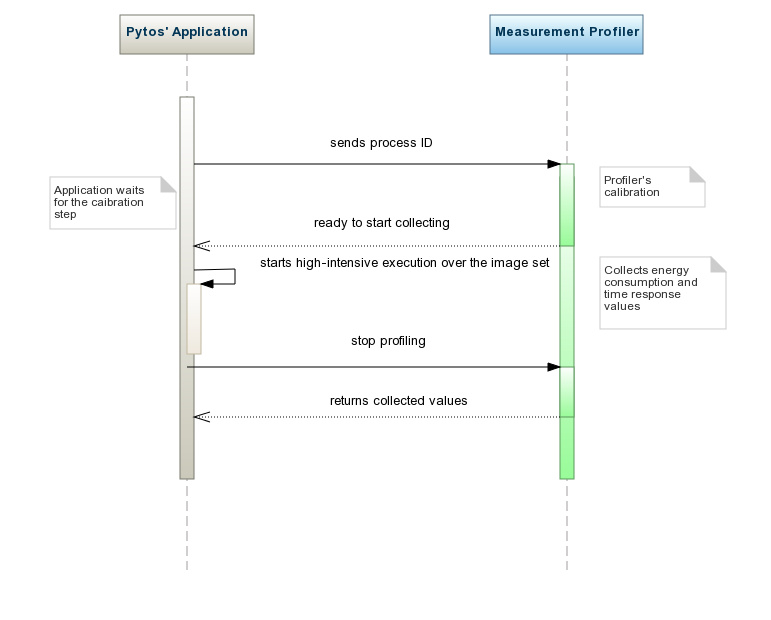
\includegraphics[scale=0.45]{Figures/experimentalEnvironment.jpg}
 \caption{Metodología para la medición}
 \label{fig:experimentalSetup}
\end{figure}

%\subsection{Application Sample}
\subsection{Escenarios de Evaluación}
\label{subsec:appsample}
Evaluamos la migración de tareas pesadas usando una aplicación de reconocimiento de rostros. Como mencionamos anteriormente, los desarrolladores 
deberán seleccionar en fase de diseño, los métodos costosos computacionalmente. Claramente, en este caso la operación que más necesita de recursos
es la de reconocimiento de rostros. De tal forma, si el cómputo es enviado a un \textit{cloudlet}, la aplicación principal espera por la respuesta
a fin de ser mostrado en el dispositivo limitado. 
En el cuadro~\ref{table:imageSet} se muestra el conjunto de imágenes que fueron probados con nuestra aplicación. Cada conjunto contiene 20 
imágenes que fueron obtenidas de una misma cámara web. 

\begin{table}[]
\centering
\caption{Datos de los diferentes conjuntos de imágenes usados en la aplicación de reconocimiento de rostros}
\label{table:imageSet}
\begin{tabular}{|c|c|c|c|}
\hline
{\bf Set} & {\bf \begin{tabular}[c]{@{}c@{}}Resolution\\ (width x height)\end{tabular}} & {\bf \begin{tabular}[c]{@{}c@{}} Average size  \\ (bytes)\end{tabular}} & {\bf \begin{tabular}[c]{@{}c@{}} Standard  \\ deviation \end{tabular}} \\ \hline
1         & 160x120                                                                     & 7612                                                          & 141                                                                         \\ \hline
2         & 176x144                                                                     & 8959                                                          & 203                                                                         \\ \hline
3         & 416x240                                                                     & 21478                                                         & 1183                                                                        \\ \hline
4         & 352x288                                                                     & 23548                                                         & 1494                                                                        \\ \hline
5         & 800x600                                                                     & 84668                                                         & 810                                                                         \\ \hline
6         & 960x544                                                                     & 89023                                                         & 5098                                                                        \\ \hline
\end{tabular}
\end{table}

\subsection{Resultados Iniciales}



\begin{figure}
\centering
 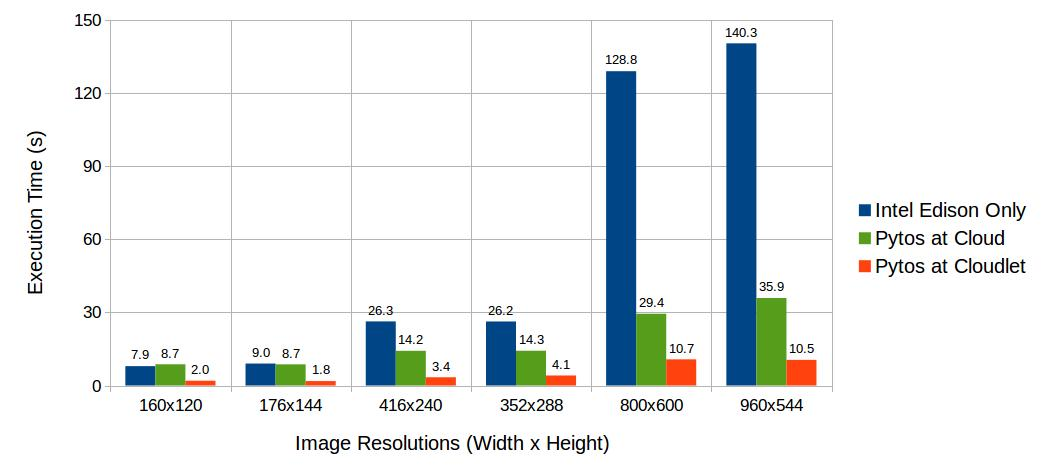
\includegraphics[scale=0.35]{Figures/timeRepsonseBenchmark}
 \caption{Comparación de tiempo de respuestas usando diferentes escenarios.}
 \label{fig:timesResponseBenchmark}
\end{figure}

\begin{figure}
\centering
 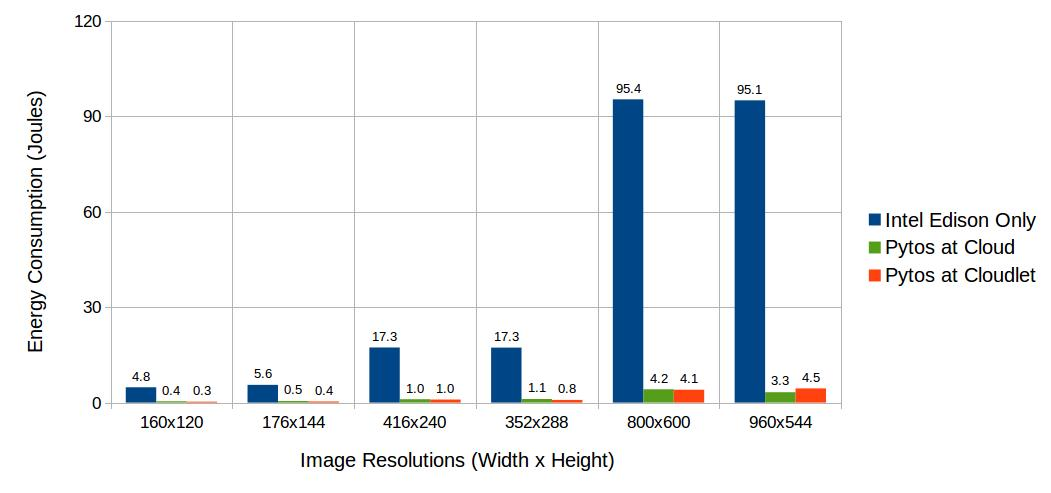
\includegraphics[scale=0.35]{Figures/energyBenchmark}
 \caption{Comparación de energía consumida usando diferentes escenarios.}
 \label{fig:energyBenchmark}
\end{figure}
%modified
Se evaluó localmente (cliente) y remotamente (\textit{cloudlet} y nube) el rendimiento y el ahorro de energía de una aplicación que usualmente consume abundantes recursos (descrito en 
la Sección~\ref{subsec:appsample}). Los experimentos son ejecutados en tres escenarios: (1)solamente en el dispositivo Intel Edison (2)
en la infraestructura \textit{cloudlet}, y (3) sobre la infraestructura en nube. El último escenario no es un objetivo del framework propuesto,
sin embargo, lo consideramos para notar el impacto de la demora en los escenarios WAN. 

La Figura~\ref{subsec:appsample} muestra la diferencia de rendimiento al procesar los conjuntos (1), (2) y (3) de las
imágenes variables (Cuadro \ref{table:imageSet}). Como se esperaba, a medida que la imagen de entrada a ser procesada era más grande, más tiempo
se requería para su procesamiento; en todos los escenarios. Por ejemplo, para la ejecución aislada en Intel Edison varía desde 7.94 segundos (s)
(con una desviación estándar de  0.0215) para procesar el conjunto 1 de imágenes más liviano a 140 s (con una desviación estándar de 0.2571)
para procesar el conjunto más pesado. Mientras tanto, empleando la infraestructura \textit{cloudlet} se utilizó 1.98 s (con una desviación estándar de
0.4839) para procesar el conjunto 1, y 10.53 s para procesar el conjunto 6, eso significa que el rendimiento se acrecentó en un factor de
4 a 13 veces. Los experimentos usando la nube muestran un rendimiento bueno en comparación con la ejecución aislada en Intel Edison, pero son peores
en comparación con los ejecutados en entornos \textit{cloudlets} debido a la latencia WAN elevada. Por lo que se confirma que la ejecución de 
tareas pesadas en \textit{cloudlets} es una mejor apuesta.

Similarmente, la Figura~\ref{fig:energyBenchmark} muestra la misma tendencia en ahorro de energía. La energía en ejecución aislada en 
Intel Edison varía desde 4.81 Joules (J) (con una desviación estándar de 0.0822) para procesar el conjunto 1, a 95.06 J
(con una desviación estándar de 0.3077) para procesar el último conjunto de imágenes 6. Por otra parte, migrando cómputo al \textit{cloudlet}
varía de  0.29 J (con una desviación estándar de 0.0217) para procesar el conjunto 1 (economizando energía en un factor de 16), a 4,45 J (desviación
estándar de 0.1884) para procesar el conjunto 6 (economizando energía en un factor de 21).

 
% Chapter 6

\chapter{Cronograma de Trabajo} % Main chapter title

\label{ch:Chapter7} % For referencing the chapter elsewhere, use \ref{Chapter1} 

\lhead{Capítulo 7. \emph{Cronograma de Trabajo}} % This is for the header on each page - perhaps a shortened title

%----------------------------------------------------------------------------------------
\begin{table}[h]
 \begin{tabular}{|l|c|c|c|c|c|c|c|c|c|}
\hline
\multicolumn{1}{|c|}{\multirow{3}{*}{Actividades}}                                          & \multicolumn{9}{c|}{Años y Semestres}                                                                                                                                                                                                                  \\ \cline{2-10} 
\multicolumn{1}{|c|}{}                                                                      & \multicolumn{2}{l|}{2014}                       & \multicolumn{5}{c|}{2015}                                                                                                                & \multicolumn{2}{c|}{2016}                                 \\ \cline{2-10} 
\multicolumn{1}{|c|}{}                                                                      & \multicolumn{1}{l|}{1} & \multicolumn{1}{l|}{2} & \multicolumn{1}{l|}{Febrero} & \multicolumn{1}{l|}{Marzo} & \multicolumn{1}{l|}{Abril} & \multicolumn{1}{l|}{1} & \multicolumn{1}{l|}{2} & \multicolumn{1}{l|}{Enero} & \multicolumn{1}{l|}{Febrero} \\ \hline
Disciplinas Obligatorias                                                                    & \checkmark                      & \checkmark                      &                              &                            &                            & \checkmark                       & \boxing                      &                            &                              \\ \hline
\begin{tabular}[c]{@{}l@{}}Estudio de la Bibliografía \\ y estado del Arte\end{tabular} &                        &                        &\checkmark                               &\checkmark                             & \checkmark                           &                      &                        &                            &                              \\ \hline
\begin{tabular}[c]{@{}l@{}}Estudio de métricas de \\ evaluación\end{tabular}               &                        &                        &                              &                            &\checkmark                             &\checkmark                         &                       &                           &                              \\ \hline
\begin{tabular}[c]{@{}l@{}}Implementación de \\ propuestas\end{tabular}                     &                        &                        &                              &                            &                            &\checkmark                         & \boxing                       &                            &                              \\ \hline
\begin{tabular}[c]{@{}l@{}}Presentación de Artículos \end{tabular}             &                        &                        &                              &                            &                            & \checkmark                       & \boxing                      & \boxing                           &                              \\ \hline
\begin{tabular}[c]{@{}l@{}}Redacción de la tesis \\ y defensa\end{tabular}                  &                        &                        &                              &                            &                            &                        & \boxing                       & \boxing                          & \boxing                            \\ \hline
\end{tabular}
\caption{Plan de trabajo}
\end{table}



% Chapter 8

\chapter{Conclusiones} % Main chapter title

\label{ch:Chapter8} % For referencing the chapter elsewhere, use \ref{Chapter1} 

\lhead{Capítulo 8. \emph{Conclusiones}} % This is for the header on each page - perhaps a shortened title

%----------------------------------------------------------------------------------------
En este trabajo se propone Pytos, un framework para emplear \textit{offloading} en entornos \textit{cloudlet}, lo cual permitirá ahorrar 
energía y optimizar el rendimiento de aplicaciones móviles que consuman abundantes recursos. Nuestro enfoque lleva la computación al borde de 
la red y visiona solucionar una de las principales limitaciones de los frameworks basados en nube: la demora de las redes WAN. 

La arquitectura propuesta es transparente para los usuarios finales, ya que descubre los \textit{cloudlets} disponibles y decide si
el \textit{offloading} es factible , o no, de manera automática. A los desarrolladores, nuestro modelo permitirá una integración simple y una 
migración de código de grano fino usando decoradores de Python. Como fue demostrado en las evaluaciones empíricas, la migración de cómputo 
a los \textit{cloudlets} puede conservar energía hasta un factor de 20.


%Furthermore, before sending computation to cloudlet mobile-context characteristics are taken in consideration (network state and history-based execution time). 
Además, la arquitectura propuesta puede ser ampliamente usada. Cada aplicación que precise de recursos adicionales (codificación de video, procesamiento
de señales, juegos, etc. ) puede ser asistida la computación en el borde de la red. Sin embargo, en el modelo propuesto, el desarrollador 
escoger la tarea conveniente que pueda ser migrada sin efectos secundarios en la aplicación. Por ejemplo, un método no puede ser migrado si este 
requiere llamadas al sistema operativo, como lecturas de sensores, uso de instrucciones de Entrada/Salida, o consultas a base de datos locales. 
En versiones futuras, se visiona solucionar tales limitaciones.

La arquitectura Pytos, si es desplegada cerca a entornos de red inalámbricas, puede mejorar la experiencia de usuario, ofreciendo, por ejemplo, 
un mejor servicio en áreas comerciales, como cafeterías, centros comerciales, y restaurantes. Si es desplegado ampliamente, 
los \textit{cloudlets} pueden reducir el tráfico de internet a nivel global. 

 

%----------------------------------------------------------------------------------------
%	THESIS CONTENT - APPENDICES
%----------------------------------------------------------------------------------------

\addtocontents{toc}{\vspace{2em}} % Add a gap in the Contents, for aesthetics

\appendix % Cue to tell LaTeX that the following 'chapters' are Appendices

% Include the appendices of the thesis as separate files from the Appendices folder
% Uncomment the lines as you write the Appendices

%% Appendix A

\chapter{Appendix Title Here} % Main appendix title

\label{AppendixA} % For referencing this appendix elsewhere, use \ref{AppendixA}

\lhead{Appendix A. \emph{Appendix Title Here}} % This is for the header on each page - perhaps a shortened title

Write your Appendix content here.
%\input{Appendices/AppendixB}
%\input{Appendices/AppendixC}

\addtocontents{toc}{\vspace{2em}} % Add a gap in the Contents, for aesthetics

\backmatter

%----------------------------------------------------------------------------------------
%	BIBLIOGRAPHY
%----------------------------------------------------------------------------------------

\label{Bibliography}

\lhead{\emph{Bibliography}} % Change the page header to say "Bibliography"

\bibliographystyle{unsrtnat} % Use the "unsrtnat" BibTeX style for formatting the Bibliography

\bibliography{Bibliography2} % The references (bibliography) information are stored in the file named "Bibliography.bib"

%\bibliography{main}

\end{document}  